\documentclass[11pt]{article}
\usepackage[utf8]{inputenc}
\usepackage[T1]{fontenc}
\usepackage{textcomp}
\usepackage[a4paper,margin=2.1cm]{geometry}
\usepackage{amsmath,amssymb}
\usepackage{graphicx}
\usepackage{tikz}
\usetikzlibrary{arrows.meta}
\usepackage{xcolor}
\usepackage{mdframed}
\usepackage[colorlinks=true,linkcolor=blue!60!black]{hyperref}
\setlength{\parindent}{0pt}
\setlength{\parskip}{6pt}

\newcommand{\question}[1]{\par\medskip\noindent\textbf{#1}\par}
\newmdenv[linecolor=green!45!black,linewidth=0.8pt,backgroundcolor=green!4,
  innertopmargin=4pt,innerbottommargin=4pt,skipabove=6pt,skipbelow=6pt]{answerbox}

\title{\textbf{Line Segments}\\[0.3em]\large Worked Solutions with TikZ Graphs}
\author{Wisest Maths --- Year 1 A-Level, Coordinate Geometry (ref \texttt{cg2})}
\date{}

\begin{document}
\maketitle
\noindent This document contains all 70 \emph{Line Segments} questions, each with a fully worked
solution and a TikZ diagram on the coordinate plane: endpoints, segments, midpoints, points of division,
triangles, quadrilaterals and circles are all plotted. Several \emph{find the unknown coordinate} questions
are shown as \emph{locus} diagrams --- a fixed point with a line and a circle whose intersections are the
solutions.
\tableofcontents
\bigskip
\hrule

\section*{Line Segments 01\quad\small\texttt{(cg2-001)}}
\addcontentsline{toc}{section}{Line Segments 01 (cg2-001)}
\textit{Difficulty: Foundation \quad\textbar\quad Marks: 4}

\question{Find both (i) the midpoint and (ii) the exact length of the segment from \( (-2, 4) \) to \( (4, 12) \).}

\textbf{Worked solution.}

\textit{Step 1: (i) Midpoint:}
\[\begin{gathered}
M = \left(\dfrac{-2 + 4}{2},\ \dfrac{4 + 12}{2}\right) = (1,\ 8)
\end{gathered}\]
Using the midpoint formula: average the x-coordinates and average the y-coordinates separately.

\textit{Step 2: (ii) Length:}
\[\begin{gathered}
d = \sqrt{(4 - (-2))^2 + (12 - 4)^2} = \sqrt{36 + 64} = \sqrt{100} = 10
\end{gathered}\]
The distance formula comes from Pythagoras applied to the horizontal and vertical differences. Note that 4 - (-2) = 6, not 2 --- be careful with double negatives.

\begin{answerbox}
\textbf{Final answer:}\quad (i) \(\displaystyle M = (1, 8)\); (ii) \(\displaystyle d = 10\)
\end{answerbox}
\textbf{Diagram.}

\begin{center}
\resizebox{\ifdim\width>\linewidth \linewidth\else \width\fi}{!}{%
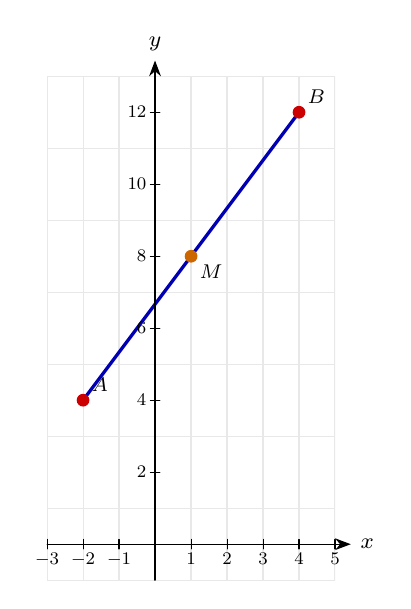
\begin{tikzpicture}[>={Stealth[length=2mm]},font=\footnotesize,line cap=round]
\begin{scope}
\clip (0,0) rectangle (3.657,6.4);
\draw[gray!18] (0,-0.457) grid[xstep=0.457,ystep=0.914] (3.657,6.4);
\draw[blue!70!black,very thick] (0.457,2.286) -- (3.2,5.943);
\end{scope}
\draw[->] (0,0.457) -- (3.857,0.457) node[right]{$x$};
\draw[->] (1.371,0) -- (1.371,6.6) node[above]{$y$};
\draw (0,0.397) -- (0,0.517) node[below=2pt,scale=0.8]{$-3$};
\draw (0.457,0.397) -- (0.457,0.517) node[below=2pt,scale=0.8]{$-2$};
\draw (0.914,0.397) -- (0.914,0.517) node[below=2pt,scale=0.8]{$-1$};
\draw (1.829,0.397) -- (1.829,0.517) node[below=2pt,scale=0.8]{$1$};
\draw (2.286,0.397) -- (2.286,0.517) node[below=2pt,scale=0.8]{$2$};
\draw (2.743,0.397) -- (2.743,0.517) node[below=2pt,scale=0.8]{$3$};
\draw (3.2,0.397) -- (3.2,0.517) node[below=2pt,scale=0.8]{$4$};
\draw (3.657,0.397) -- (3.657,0.517) node[below=2pt,scale=0.8]{$5$};
\draw (1.311,1.371) -- (1.431,1.371) node[left=2pt,scale=0.8]{$2$};
\draw (1.311,2.286) -- (1.431,2.286) node[left=2pt,scale=0.8]{$4$};
\draw (1.311,3.2) -- (1.431,3.2) node[left=2pt,scale=0.8]{$6$};
\draw (1.311,4.114) -- (1.431,4.114) node[left=2pt,scale=0.8]{$8$};
\draw (1.311,5.029) -- (1.431,5.029) node[left=2pt,scale=0.8]{$10$};
\draw (1.311,5.943) -- (1.431,5.943) node[left=2pt,scale=0.8]{$12$};
\fill[red!80!black] (0.457,2.286) circle (2.3pt);
\node[above right,scale=0.9] at (0.457,2.286) {$A$};
\fill[red!80!black] (3.2,5.943) circle (2.3pt);
\node[above right,scale=0.9] at (3.2,5.943) {$B$};
\fill[orange!80!black] (1.829,4.114) circle (2.3pt);
\node[below right,scale=0.9] at (1.829,4.114) {$M$};
\end{tikzpicture}
}
\end{center}
\small The points and segments shown on the coordinate plane.\normalsize

\medskip\hrule

\section*{Line Segments 02\quad\small\texttt{(cg2-002)}}
\addcontentsline{toc}{section}{Line Segments 02 (cg2-002)}
\textit{Difficulty: Foundation \quad\textbar\quad Marks: 4}

\question{Find both (i) the midpoint and (ii) the exact length of the segment from \( (3, -5) \) to \( (-3, 3) \).}

\textbf{Worked solution.}

\textit{Step 1: (i) Midpoint:}
\[\begin{gathered}
M = \left(\dfrac{3 + (-3)}{2},\ \dfrac{-5 + 3}{2}\right) = (0,\ -1)
\end{gathered}\]
Using the midpoint formula: average the x-coordinates and average the y-coordinates separately.

\textit{Step 2: (ii) Length:}
\[\begin{gathered}
d = \sqrt{(-3 - 3)^2 + (3 - (-5))^2} = \sqrt{36 + 64} = \sqrt{100} = 10
\end{gathered}\]
Using the distance formula. Note that 3 - (-5) = 8, not -2. Subtracting a negative is the same as adding.

\begin{answerbox}
\textbf{Final answer:}\quad (i) \(\displaystyle M = (0, -1)\); (ii) \(\displaystyle d = 10\)
\end{answerbox}
\textbf{Diagram.}

\begin{center}
\resizebox{\ifdim\width>\linewidth \linewidth\else \width\fi}{!}{%
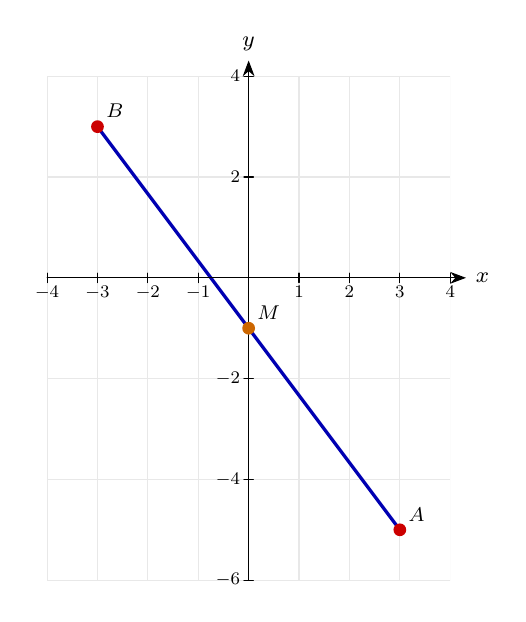
\begin{tikzpicture}[>={Stealth[length=2mm]},font=\footnotesize,line cap=round]
\begin{scope}
\clip (0,0) rectangle (5.12,6.4);
\draw[gray!18] (0,0) grid[xstep=0.64,ystep=1.28] (5.12,6.4);
\draw[blue!70!black,very thick] (4.48,0.64) -- (0.64,5.76);
\end{scope}
\draw[->] (0,3.84) -- (5.32,3.84) node[right]{$x$};
\draw[->] (2.56,0) -- (2.56,6.6) node[above]{$y$};
\draw (0,3.78) -- (0,3.9) node[below=2pt,scale=0.8]{$-4$};
\draw (0.64,3.78) -- (0.64,3.9) node[below=2pt,scale=0.8]{$-3$};
\draw (1.28,3.78) -- (1.28,3.9) node[below=2pt,scale=0.8]{$-2$};
\draw (1.92,3.78) -- (1.92,3.9) node[below=2pt,scale=0.8]{$-1$};
\draw (3.2,3.78) -- (3.2,3.9) node[below=2pt,scale=0.8]{$1$};
\draw (3.84,3.78) -- (3.84,3.9) node[below=2pt,scale=0.8]{$2$};
\draw (4.48,3.78) -- (4.48,3.9) node[below=2pt,scale=0.8]{$3$};
\draw (5.12,3.78) -- (5.12,3.9) node[below=2pt,scale=0.8]{$4$};
\draw (2.5,0) -- (2.62,0) node[left=2pt,scale=0.8]{$-6$};
\draw (2.5,1.28) -- (2.62,1.28) node[left=2pt,scale=0.8]{$-4$};
\draw (2.5,2.56) -- (2.62,2.56) node[left=2pt,scale=0.8]{$-2$};
\draw (2.5,5.12) -- (2.62,5.12) node[left=2pt,scale=0.8]{$2$};
\draw (2.5,6.4) -- (2.62,6.4) node[left=2pt,scale=0.8]{$4$};
\fill[red!80!black] (4.48,0.64) circle (2.3pt);
\node[above right,scale=0.9] at (4.48,0.64) {$A$};
\fill[red!80!black] (0.64,5.76) circle (2.3pt);
\node[above right,scale=0.9] at (0.64,5.76) {$B$};
\fill[orange!80!black] (2.56,3.2) circle (2.3pt);
\node[above right,scale=0.9] at (2.56,3.2) {$M$};
\end{tikzpicture}
}
\end{center}
\small The points and segments shown on the coordinate plane.\normalsize

\medskip\hrule

\section*{Line Segments 03\quad\small\texttt{(cg2-003)}}
\addcontentsline{toc}{section}{Line Segments 03 (cg2-003)}
\textit{Difficulty: Foundation \quad\textbar\quad Marks: 4}

\question{Find the exact length of the segment of the line \( y = 3x + 1 \) between \( x = 2 \) and \( x = 5 \).}

\textbf{Worked solution.}

\textit{Step 1: Find the \( y \)-coordinates at each \( x \)-value.}
\[\begin{gathered}
x = 2:\; y = 3(2) + 1 = 7 \qquad x = 5:\; y = 3(5) + 1 = 16
\end{gathered}\]
Substitute each x-value into the line equation to find the corresponding y-coordinate, giving the two endpoints.

\textit{Step 2: Apply the distance formula between \( (2, 7) \) and \( (5, 16) \).}
\[\begin{gathered}
d = \sqrt{(5 - 2)^2 + (16 - 7)^2} = \sqrt{9 + 81} = \sqrt{90} = 3\sqrt{10}
\end{gathered}\]
\(\sqrt{90} = \sqrt{9 \times 10} = 3\sqrt{10}\).

\begin{answerbox}
\textbf{Final answer:}\quad \(\displaystyle d = 3\sqrt{10}\)
\end{answerbox}
\textbf{Diagram.}

\begin{center}
\resizebox{\ifdim\width>\linewidth \linewidth\else \width\fi}{!}{%
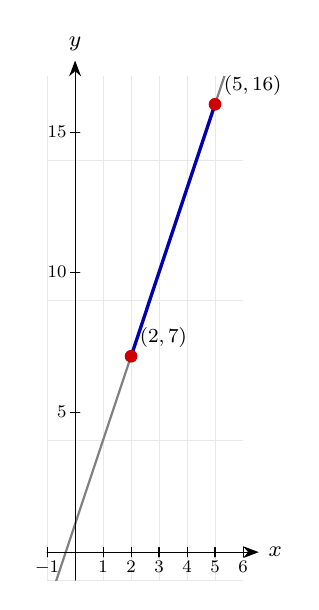
\begin{tikzpicture}[>={Stealth[length=2mm]},font=\footnotesize,line cap=round]
\begin{scope}
\clip (0,0) rectangle (2.489,6.4);
\draw[gray!18] (0,-1.422) grid[xstep=0.356,ystep=1.778] (2.489,6.4);
\draw[gray,thick] (0,-0.356) -- (2.489,7.111);
\draw[blue!70!black,very thick] (1.067,2.844) -- (2.133,6.044);
\end{scope}
\draw[->] (0,0.356) -- (2.689,0.356) node[right]{$x$};
\draw[->] (0.356,0) -- (0.356,6.6) node[above]{$y$};
\draw (0,0.296) -- (0,0.416) node[below=2pt,scale=0.8]{$-1$};
\draw (0.711,0.296) -- (0.711,0.416) node[below=2pt,scale=0.8]{$1$};
\draw (1.067,0.296) -- (1.067,0.416) node[below=2pt,scale=0.8]{$2$};
\draw (1.422,0.296) -- (1.422,0.416) node[below=2pt,scale=0.8]{$3$};
\draw (1.778,0.296) -- (1.778,0.416) node[below=2pt,scale=0.8]{$4$};
\draw (2.133,0.296) -- (2.133,0.416) node[below=2pt,scale=0.8]{$5$};
\draw (2.489,0.296) -- (2.489,0.416) node[below=2pt,scale=0.8]{$6$};
\draw (0.296,2.133) -- (0.416,2.133) node[left=2pt,scale=0.8]{$5$};
\draw (0.296,3.911) -- (0.416,3.911) node[left=2pt,scale=0.8]{$10$};
\draw (0.296,5.689) -- (0.416,5.689) node[left=2pt,scale=0.8]{$15$};
\fill[red!80!black] (1.067,2.844) circle (2.3pt);
\node[above right,scale=0.9] at (1.067,2.844) {$(2,7)$};
\fill[red!80!black] (2.133,6.044) circle (2.3pt);
\node[above right,scale=0.9] at (2.133,6.044) {$(5,16)$};
\end{tikzpicture}
}
\end{center}
\small The points and segments shown on the coordinate plane.\normalsize

\medskip\hrule

\section*{Line Segments 04\quad\small\texttt{(cg2-004)}}
\addcontentsline{toc}{section}{Line Segments 04 (cg2-004)}
\textit{Difficulty: Foundation \quad\textbar\quad Marks: 4}

\question{Find the exact length of the segment of the line \( y = -2x + 7 \) between \( x = 1 \) and \( x = 4 \).}

\textbf{Worked solution.}

\textit{Step 1: Find the \( y \)-coordinates.}
\[\begin{gathered}
x = 1:\; y = -2(1) + 7 = 5 \qquad x = 4:\; y = -2(4) + 7 = -1
\end{gathered}\]
Substitute each x-value into the equation to find the two endpoints of the segment.

\textit{Step 2: Apply the distance formula between \( (1, 5) \) and \( (4, -1) \).}
\[\begin{gathered}
d = \sqrt{(4 - 1)^2 + (-1 - 5)^2} = \sqrt{9 + 36} = \sqrt{45} = 3\sqrt{5}
\end{gathered}\]
\(\sqrt{45} = \sqrt{9 \times 5} = 3\sqrt{5}\).

\begin{answerbox}
\textbf{Final answer:}\quad \(\displaystyle d = 3\sqrt{5}\)
\end{answerbox}
\textbf{Diagram.}

\begin{center}
\resizebox{\ifdim\width>\linewidth \linewidth\else \width\fi}{!}{%
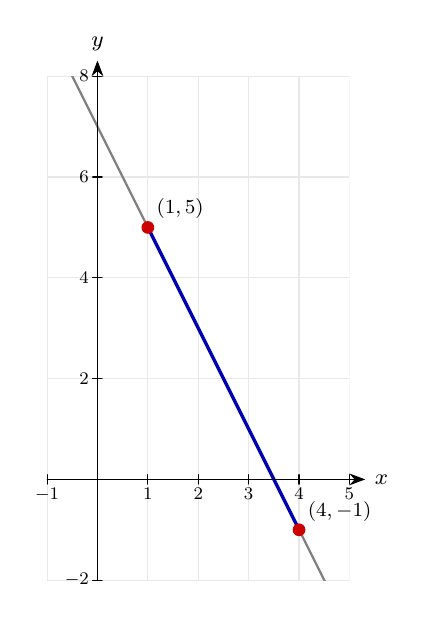
\begin{tikzpicture}[>={Stealth[length=2mm]},font=\footnotesize,line cap=round]
\begin{scope}
\clip (0,0) rectangle (3.84,6.4);
\draw[gray!18] (0,0) grid[xstep=0.64,ystep=1.28] (3.84,6.4);
\draw[gray,thick] (0,7.04) -- (3.84,-0.64);
\draw[blue!70!black,very thick] (1.28,4.48) -- (3.2,0.64);
\end{scope}
\draw[->] (0,1.28) -- (4.04,1.28) node[right]{$x$};
\draw[->] (0.64,0) -- (0.64,6.6) node[above]{$y$};
\draw (0,1.22) -- (0,1.34) node[below=2pt,scale=0.8]{$-1$};
\draw (1.28,1.22) -- (1.28,1.34) node[below=2pt,scale=0.8]{$1$};
\draw (1.92,1.22) -- (1.92,1.34) node[below=2pt,scale=0.8]{$2$};
\draw (2.56,1.22) -- (2.56,1.34) node[below=2pt,scale=0.8]{$3$};
\draw (3.2,1.22) -- (3.2,1.34) node[below=2pt,scale=0.8]{$4$};
\draw (3.84,1.22) -- (3.84,1.34) node[below=2pt,scale=0.8]{$5$};
\draw (0.58,0) -- (0.7,0) node[left=2pt,scale=0.8]{$-2$};
\draw (0.58,2.56) -- (0.7,2.56) node[left=2pt,scale=0.8]{$2$};
\draw (0.58,3.84) -- (0.7,3.84) node[left=2pt,scale=0.8]{$4$};
\draw (0.58,5.12) -- (0.7,5.12) node[left=2pt,scale=0.8]{$6$};
\draw (0.58,6.4) -- (0.7,6.4) node[left=2pt,scale=0.8]{$8$};
\fill[red!80!black] (1.28,4.48) circle (2.3pt);
\node[above right,scale=0.9] at (1.28,4.48) {$(1,5)$};
\fill[red!80!black] (3.2,0.64) circle (2.3pt);
\node[above right,scale=0.9] at (3.2,0.64) {$(4,-1)$};
\end{tikzpicture}
}
\end{center}
\small The points and segments shown on the coordinate plane.\normalsize

\medskip\hrule

\section*{Line Segments 05\quad\small\texttt{(cg2-005)}}
\addcontentsline{toc}{section}{Line Segments 05 (cg2-005)}
\textit{Difficulty: Foundation \quad\textbar\quad Marks: 5}

\question{Find the midpoint and exact length of the segment of \( y = \dfrac{1}{2}x - 3 \) between \( x = 2 \) and \( x = 10 \).}

\textbf{Worked solution.}

\textit{Step 1: Find the endpoints.}
\[\begin{gathered}
x = 2:\; y = \tfrac{1}{2}(2) - 3 = -2 \qquad x = 10:\; y = \tfrac{1}{2}(10) - 3 = 2
\end{gathered}\]
Points are \( A(2, -2) \) and \( B(10, 2) \).

\textit{Step 2: Midpoint:}
\[\begin{gathered}
M = \left(\dfrac{2 + 10}{2},\ \dfrac{-2 + 2}{2}\right) = (6,\ 0)
\end{gathered}\]
Using the midpoint formula. The y-coordinates cancel (-2 + 2 = 0), so the midpoint lies on the x-axis.

\textit{Step 3: Length:}
\[\begin{gathered}
d = \sqrt{(10 - 2)^2 + (2 - (-2))^2} = \sqrt{64 + 16} = \sqrt{80} = 4\sqrt{5}
\end{gathered}\]
\(\sqrt{80} = \sqrt{16 \times 5} = 4\sqrt{5}\).

\begin{answerbox}
\textbf{Final answer:}\quad \(\displaystyle M = (6, 0) ;  d = 4\sqrt{5}\)
\end{answerbox}
\textbf{Diagram.}

\begin{center}
\resizebox{\ifdim\width>\linewidth \linewidth\else \width\fi}{!}{%
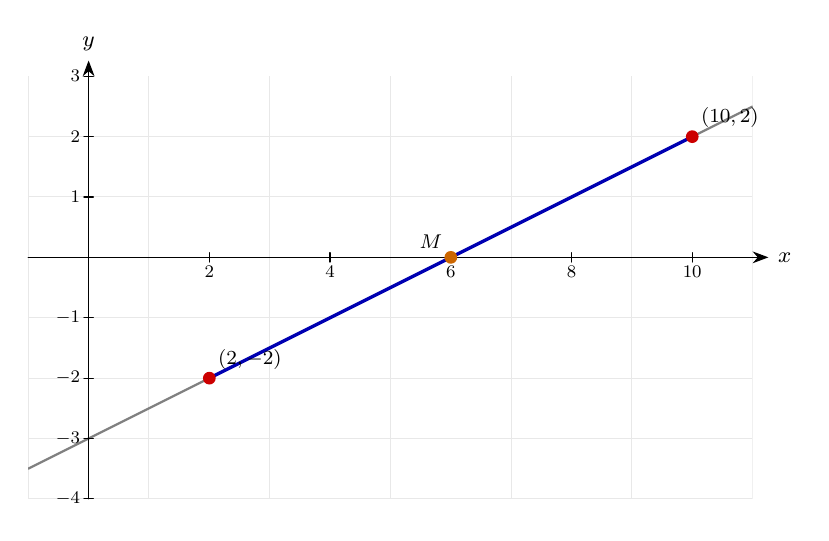
\begin{tikzpicture}[>={Stealth[length=2mm]},font=\footnotesize,line cap=round]
\begin{scope}
\clip (0,0) rectangle (9.2,5.367);
\draw[gray!18] (-0.767,0) grid[xstep=1.533,ystep=0.767] (9.2,5.367);
\draw[gray,thick] (0,0.383) -- (9.2,4.983);
\draw[blue!70!black,very thick] (2.3,1.533) -- (8.433,4.6);
\end{scope}
\draw[->] (0,3.067) -- (9.4,3.067) node[right]{$x$};
\draw[->] (0.767,0) -- (0.767,5.567) node[above]{$y$};
\draw (2.3,3.007) -- (2.3,3.127) node[below=2pt,scale=0.8]{$2$};
\draw (3.833,3.007) -- (3.833,3.127) node[below=2pt,scale=0.8]{$4$};
\draw (5.367,3.007) -- (5.367,3.127) node[below=2pt,scale=0.8]{$6$};
\draw (6.9,3.007) -- (6.9,3.127) node[below=2pt,scale=0.8]{$8$};
\draw (8.433,3.007) -- (8.433,3.127) node[below=2pt,scale=0.8]{$10$};
\draw (0.707,0) -- (0.827,0) node[left=2pt,scale=0.8]{$-4$};
\draw (0.707,0.767) -- (0.827,0.767) node[left=2pt,scale=0.8]{$-3$};
\draw (0.707,1.533) -- (0.827,1.533) node[left=2pt,scale=0.8]{$-2$};
\draw (0.707,2.3) -- (0.827,2.3) node[left=2pt,scale=0.8]{$-1$};
\draw (0.707,3.833) -- (0.827,3.833) node[left=2pt,scale=0.8]{$1$};
\draw (0.707,4.6) -- (0.827,4.6) node[left=2pt,scale=0.8]{$2$};
\draw (0.707,5.367) -- (0.827,5.367) node[left=2pt,scale=0.8]{$3$};
\fill[red!80!black] (2.3,1.533) circle (2.3pt);
\node[above right,scale=0.9] at (2.3,1.533) {$(2,-2)$};
\fill[red!80!black] (8.433,4.6) circle (2.3pt);
\node[above right,scale=0.9] at (8.433,4.6) {$(10,2)$};
\fill[orange!80!black] (5.367,3.067) circle (2.3pt);
\node[above left,scale=0.9] at (5.367,3.067) {$M$};
\end{tikzpicture}
}
\end{center}
\small The points and segments shown on the coordinate plane.\normalsize

\medskip\hrule

\section*{Line Segments 06\quad\small\texttt{(cg2-006)}}
\addcontentsline{toc}{section}{Line Segments 06 (cg2-006)}
\textit{Difficulty: Foundation \quad\textbar\quad Marks: 4}

\question{Find the exact length of the segment of the line \( 2x + y - 4 = 0 \) between \( x = 0 \) and \( x = 3 \).}

\textbf{Worked solution.}

\textit{Step 1: Rearrange the line to \( y = -2x + 4 \), then find the endpoints.}
\[\begin{gathered}
x = 0:\; y = 4 \qquad x = 3:\; y = -2(3) + 4 = -2
\end{gathered}\]
Rearrange the equation to make y the subject first, then substitute each x-value to find the endpoints.

\textit{Step 2: Apply the distance formula between \( (0, 4) \) and \( (3, -2) \).}
\[\begin{gathered}
d = \sqrt{(3 - 0)^2 + (-2 - 4)^2} = \sqrt{9 + 36} = \sqrt{45} = 3\sqrt{5}
\end{gathered}\]
Simplify the surd: find the largest perfect square factor of 45, which is 9.

\begin{answerbox}
\textbf{Final answer:}\quad \(\displaystyle d = 3\sqrt{5}\)
\end{answerbox}
\textbf{Diagram.}

\begin{center}
\resizebox{\ifdim\width>\linewidth \linewidth\else \width\fi}{!}{%
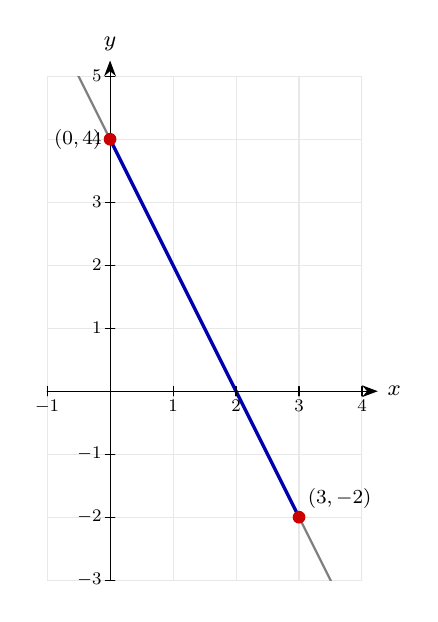
\begin{tikzpicture}[>={Stealth[length=2mm]},font=\footnotesize,line cap=round]
\begin{scope}
\clip (0,0) rectangle (4,6.4);
\draw[gray!18] (0,0) grid[xstep=0.8,ystep=0.8] (4,6.4);
\draw[gray,thick] (0,7.2) -- (4,-0.8);
\draw[blue!70!black,very thick] (0.8,5.6) -- (3.2,0.8);
\end{scope}
\draw[->] (0,2.4) -- (4.2,2.4) node[right]{$x$};
\draw[->] (0.8,0) -- (0.8,6.6) node[above]{$y$};
\draw (0,2.34) -- (0,2.46) node[below=2pt,scale=0.8]{$-1$};
\draw (1.6,2.34) -- (1.6,2.46) node[below=2pt,scale=0.8]{$1$};
\draw (2.4,2.34) -- (2.4,2.46) node[below=2pt,scale=0.8]{$2$};
\draw (3.2,2.34) -- (3.2,2.46) node[below=2pt,scale=0.8]{$3$};
\draw (4,2.34) -- (4,2.46) node[below=2pt,scale=0.8]{$4$};
\draw (0.74,0) -- (0.86,0) node[left=2pt,scale=0.8]{$-3$};
\draw (0.74,0.8) -- (0.86,0.8) node[left=2pt,scale=0.8]{$-2$};
\draw (0.74,1.6) -- (0.86,1.6) node[left=2pt,scale=0.8]{$-1$};
\draw (0.74,3.2) -- (0.86,3.2) node[left=2pt,scale=0.8]{$1$};
\draw (0.74,4) -- (0.86,4) node[left=2pt,scale=0.8]{$2$};
\draw (0.74,4.8) -- (0.86,4.8) node[left=2pt,scale=0.8]{$3$};
\draw (0.74,5.6) -- (0.86,5.6) node[left=2pt,scale=0.8]{$4$};
\draw (0.74,6.4) -- (0.86,6.4) node[left=2pt,scale=0.8]{$5$};
\fill[red!80!black] (0.8,5.6) circle (2.3pt);
\node[left,scale=0.9] at (0.8,5.6) {$(0,4)$};
\fill[red!80!black] (3.2,0.8) circle (2.3pt);
\node[above right,scale=0.9] at (3.2,0.8) {$(3,-2)$};
\end{tikzpicture}
}
\end{center}
\small The points and segments shown on the coordinate plane.\normalsize

\medskip\hrule

\section*{Line Segments 07\quad\small\texttt{(cg2-007)}}
\addcontentsline{toc}{section}{Line Segments 07 (cg2-007)}
\textit{Difficulty: Foundation \quad\textbar\quad Marks: 5}

\question{Find the midpoint and exact length of the segment of \( x + 2y - 8 = 0 \) between \( x = 2 \) and \( x = 6 \).}

\textbf{Worked solution.}

\textit{Step 1: Rearrange: \( y = \dfrac{8 - x}{2} \). Find endpoints.}
\[\begin{gathered}
x = 2:\; y = \tfrac{6}{2} = 3 \qquad x = 6:\; y = \tfrac{2}{2} = 1
\end{gathered}\]
Points are \( A(2, 3) \) and \( B(6, 1) \).

\textit{Step 2: Midpoint:}
\[\begin{gathered}
M = \left(\dfrac{2 + 6}{2},\ \dfrac{3 + 1}{2}\right) = (4,\ 2)
\end{gathered}\]
Using the midpoint formula: average the x-coordinates and average the y-coordinates.

\textit{Step 3: Length:}
\[\begin{gathered}
d = \sqrt{(6 - 2)^2 + (1 - 3)^2} = \sqrt{16 + 4} = \sqrt{20} = 2\sqrt{5}
\end{gathered}\]
\(\sqrt{20} = \sqrt{4 \times 5} = 2\sqrt{5}\).

\begin{answerbox}
\textbf{Final answer:}\quad \(\displaystyle M = (4, 2) ;  d = 2\sqrt{5}\)
\end{answerbox}
\textbf{Diagram.}

\begin{center}
\resizebox{\ifdim\width>\linewidth \linewidth\else \width\fi}{!}{%
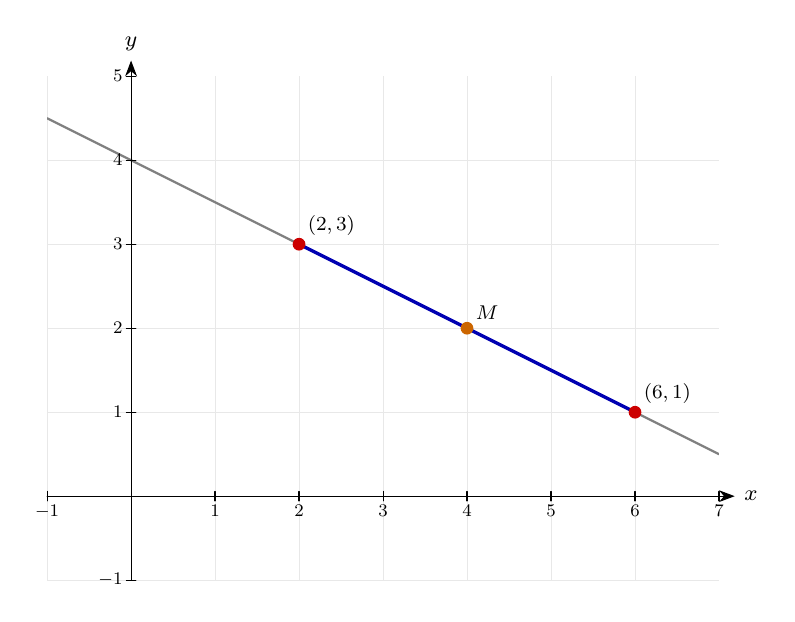
\begin{tikzpicture}[>={Stealth[length=2mm]},font=\footnotesize,line cap=round]
\begin{scope}
\clip (0,0) rectangle (8.533,6.4);
\draw[gray!18] (0,0) grid[xstep=1.067,ystep=1.067] (8.533,6.4);
\draw[gray,thick] (0,5.867) -- (8.533,1.6);
\draw[blue!70!black,very thick] (3.2,4.267) -- (7.467,2.133);
\end{scope}
\draw[->] (0,1.067) -- (8.733,1.067) node[right]{$x$};
\draw[->] (1.067,0) -- (1.067,6.6) node[above]{$y$};
\draw (0,1.007) -- (0,1.127) node[below=2pt,scale=0.8]{$-1$};
\draw (2.133,1.007) -- (2.133,1.127) node[below=2pt,scale=0.8]{$1$};
\draw (3.2,1.007) -- (3.2,1.127) node[below=2pt,scale=0.8]{$2$};
\draw (4.267,1.007) -- (4.267,1.127) node[below=2pt,scale=0.8]{$3$};
\draw (5.333,1.007) -- (5.333,1.127) node[below=2pt,scale=0.8]{$4$};
\draw (6.4,1.007) -- (6.4,1.127) node[below=2pt,scale=0.8]{$5$};
\draw (7.467,1.007) -- (7.467,1.127) node[below=2pt,scale=0.8]{$6$};
\draw (8.533,1.007) -- (8.533,1.127) node[below=2pt,scale=0.8]{$7$};
\draw (1.007,0) -- (1.127,0) node[left=2pt,scale=0.8]{$-1$};
\draw (1.007,2.133) -- (1.127,2.133) node[left=2pt,scale=0.8]{$1$};
\draw (1.007,3.2) -- (1.127,3.2) node[left=2pt,scale=0.8]{$2$};
\draw (1.007,4.267) -- (1.127,4.267) node[left=2pt,scale=0.8]{$3$};
\draw (1.007,5.333) -- (1.127,5.333) node[left=2pt,scale=0.8]{$4$};
\draw (1.007,6.4) -- (1.127,6.4) node[left=2pt,scale=0.8]{$5$};
\fill[red!80!black] (3.2,4.267) circle (2.3pt);
\node[above right,scale=0.9] at (3.2,4.267) {$(2,3)$};
\fill[red!80!black] (7.467,2.133) circle (2.3pt);
\node[above right,scale=0.9] at (7.467,2.133) {$(6,1)$};
\fill[orange!80!black] (5.333,3.2) circle (2.3pt);
\node[above right,scale=0.9] at (5.333,3.2) {$M$};
\end{tikzpicture}
}
\end{center}
\small The points and segments shown on the coordinate plane.\normalsize

\medskip\hrule

\section*{Line Segments 08\quad\small\texttt{(cg2-008)}}
\addcontentsline{toc}{section}{Line Segments 08 (cg2-008)}
\textit{Difficulty: Foundation \quad\textbar\quad Marks: 5}

\question{Find the midpoint and exact length of the segment of \( y = 4x - 3 \) between \( x = -1 \) and \( x = 2 \).}

\textbf{Worked solution.}

\textit{Step 1: Find the endpoints.}
\[\begin{gathered}
x = -1:\; y = 4(-1) - 3 = -7 \qquad x = 2:\; y = 4(2) - 3 = 5
\end{gathered}\]
Points are \( A(-1, -7) \) and \( B(2, 5) \).

\textit{Step 2: Midpoint:}
\[\begin{gathered}
M = \left(\dfrac{-1 + 2}{2},\ \dfrac{-7 + 5}{2}\right) = \left(0.5,\ -1\right)
\end{gathered}\]
Using the midpoint formula. The x-coordinate gives 1/2 = 0.5, which is fine to leave as a decimal or fraction.

\textit{Step 3: Length:}
\[\begin{gathered}
d = \sqrt{(2 - (-1))^2 + (5 - (-7))^2} = \sqrt{9 + 144} = \sqrt{153} = 3\sqrt{17}
\end{gathered}\]
\(\sqrt{153} = \sqrt{9 \times 17} = 3\sqrt{17}\).

\begin{answerbox}
\textbf{Final answer:}\quad \(\displaystyle M = (0.5,\ -1) ;  d = 3\sqrt{17}\)
\end{answerbox}
\textbf{Diagram.}

\begin{center}
\resizebox{\ifdim\width>\linewidth \linewidth\else \width\fi}{!}{%
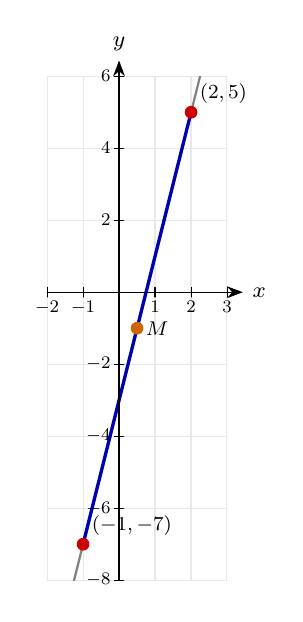
\begin{tikzpicture}[>={Stealth[length=2mm]},font=\footnotesize,line cap=round]
\begin{scope}
\clip (0,0) rectangle (2.286,6.4);
\draw[gray!18] (0,0) grid[xstep=0.457,ystep=0.914] (2.286,6.4);
\draw[gray,thick] (0,-1.371) -- (2.286,7.771);
\draw[blue!70!black,very thick] (0.457,0.457) -- (1.829,5.943);
\end{scope}
\draw[->] (0,3.657) -- (2.486,3.657) node[right]{$x$};
\draw[->] (0.914,0) -- (0.914,6.6) node[above]{$y$};
\draw (0,3.597) -- (0,3.717) node[below=2pt,scale=0.8]{$-2$};
\draw (0.457,3.597) -- (0.457,3.717) node[below=2pt,scale=0.8]{$-1$};
\draw (1.371,3.597) -- (1.371,3.717) node[below=2pt,scale=0.8]{$1$};
\draw (1.829,3.597) -- (1.829,3.717) node[below=2pt,scale=0.8]{$2$};
\draw (2.286,3.597) -- (2.286,3.717) node[below=2pt,scale=0.8]{$3$};
\draw (0.854,0) -- (0.974,0) node[left=2pt,scale=0.8]{$-8$};
\draw (0.854,0.914) -- (0.974,0.914) node[left=2pt,scale=0.8]{$-6$};
\draw (0.854,1.829) -- (0.974,1.829) node[left=2pt,scale=0.8]{$-4$};
\draw (0.854,2.743) -- (0.974,2.743) node[left=2pt,scale=0.8]{$-2$};
\draw (0.854,4.571) -- (0.974,4.571) node[left=2pt,scale=0.8]{$2$};
\draw (0.854,5.486) -- (0.974,5.486) node[left=2pt,scale=0.8]{$4$};
\draw (0.854,6.4) -- (0.974,6.4) node[left=2pt,scale=0.8]{$6$};
\fill[red!80!black] (0.457,0.457) circle (2.3pt);
\node[above right,scale=0.9] at (0.457,0.457) {$(-1,-7)$};
\fill[red!80!black] (1.829,5.943) circle (2.3pt);
\node[above right,scale=0.9] at (1.829,5.943) {$(2,5)$};
\fill[orange!80!black] (1.143,3.2) circle (2.3pt);
\node[right,scale=0.9] at (1.143,3.2) {$M$};
\end{tikzpicture}
}
\end{center}
\small The points and segments shown on the coordinate plane.\normalsize

\medskip\hrule

\section*{Line Segments 09\quad\small\texttt{(cg2-009)}}
\addcontentsline{toc}{section}{Line Segments 09 (cg2-009)}
\textit{Difficulty: Foundation \quad\textbar\quad Marks: 3}

\question{The midpoint of segment \( AB \) is \( M(3, 6) \). If \( A = (1, 2) \), find the coordinates of \( B \).}

\textbf{Worked solution.}

\textit{Step 1: Use the midpoint formula in reverse: \( x_B = 2 \times x_M - x_A \).}
\[\begin{gathered}
x_B = 2(3) - 1 = 5
\end{gathered}\]
Rearranging the midpoint formula: since the midpoint x-coordinate equals (x\_A + x\_B)/2, we get x\_B = 2 * x\_M - x\_A.

\textit{Step 2: Similarly for \( y \):}
\[\begin{gathered}
y_B = 2(6) - 2 = 10
\end{gathered}\]
Same technique for the y-coordinate: y\_B = 2 * y\_M - y\_A.

\begin{answerbox}
\textbf{Final answer:}\quad \(\displaystyle B = (5, 10)\)
\end{answerbox}
\textbf{Diagram.}

\begin{center}
\resizebox{\ifdim\width>\linewidth \linewidth\else \width\fi}{!}{%
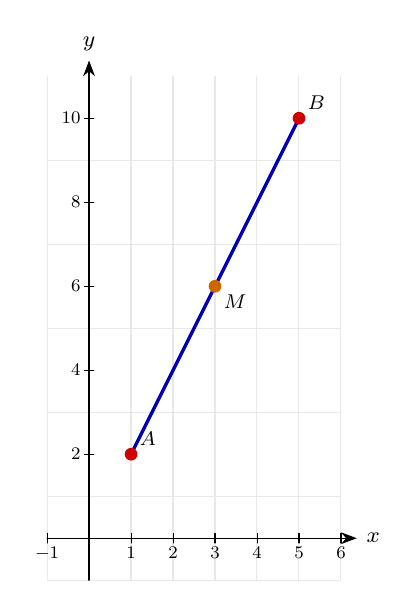
\begin{tikzpicture}[>={Stealth[length=2mm]},font=\footnotesize,line cap=round]
\begin{scope}
\clip (0,0) rectangle (3.733,6.4);
\draw[gray!18] (0,-0.533) grid[xstep=0.533,ystep=1.067] (3.733,6.4);
\draw[blue!70!black,very thick] (1.067,1.6) -- (3.2,5.867);
\end{scope}
\draw[->] (0,0.533) -- (3.933,0.533) node[right]{$x$};
\draw[->] (0.533,0) -- (0.533,6.6) node[above]{$y$};
\draw (0,0.473) -- (0,0.593) node[below=2pt,scale=0.8]{$-1$};
\draw (1.067,0.473) -- (1.067,0.593) node[below=2pt,scale=0.8]{$1$};
\draw (1.6,0.473) -- (1.6,0.593) node[below=2pt,scale=0.8]{$2$};
\draw (2.133,0.473) -- (2.133,0.593) node[below=2pt,scale=0.8]{$3$};
\draw (2.667,0.473) -- (2.667,0.593) node[below=2pt,scale=0.8]{$4$};
\draw (3.2,0.473) -- (3.2,0.593) node[below=2pt,scale=0.8]{$5$};
\draw (3.733,0.473) -- (3.733,0.593) node[below=2pt,scale=0.8]{$6$};
\draw (0.473,1.6) -- (0.593,1.6) node[left=2pt,scale=0.8]{$2$};
\draw (0.473,2.667) -- (0.593,2.667) node[left=2pt,scale=0.8]{$4$};
\draw (0.473,3.733) -- (0.593,3.733) node[left=2pt,scale=0.8]{$6$};
\draw (0.473,4.8) -- (0.593,4.8) node[left=2pt,scale=0.8]{$8$};
\draw (0.473,5.867) -- (0.593,5.867) node[left=2pt,scale=0.8]{$10$};
\fill[red!80!black] (1.067,1.6) circle (2.3pt);
\node[above right,scale=0.9] at (1.067,1.6) {$A$};
\fill[orange!80!black] (2.133,3.733) circle (2.3pt);
\node[below right,scale=0.9] at (2.133,3.733) {$M$};
\fill[red!80!black] (3.2,5.867) circle (2.3pt);
\node[above right,scale=0.9] at (3.2,5.867) {$B$};
\end{tikzpicture}
}
\end{center}
\small The points and segments shown on the coordinate plane.\normalsize

\medskip\hrule

\section*{Line Segments 10\quad\small\texttt{(cg2-010)}}
\addcontentsline{toc}{section}{Line Segments 10 (cg2-010)}
\textit{Difficulty: Foundation \quad\textbar\quad Marks: 3}

\question{The midpoint of segment \( PQ \) is \( M(-1, 4) \). If \( P = (3, 2) \), find \( Q \).}

\textbf{Worked solution.}

\textit{Step 1: Find \( x_Q \):}
\[\begin{gathered}
x_Q = 2(-1) - 3 = -5
\end{gathered}\]
Using the rearranged midpoint formula: x\_Q = 2 * x\_M - x\_P. A common mistake is to forget the factor of 2.

\textit{Step 2: Find \( y_Q \):}
\[\begin{gathered}
y_Q = 2(4) - 2 = 6
\end{gathered}\]
Same approach for the y-coordinate: y\_Q = 2 * y\_M - y\_P.

\begin{answerbox}
\textbf{Final answer:}\quad \(\displaystyle Q = (-5, 6)\)
\end{answerbox}
\textbf{Diagram.}

\begin{center}
\resizebox{\ifdim\width>\linewidth \linewidth\else \width\fi}{!}{%
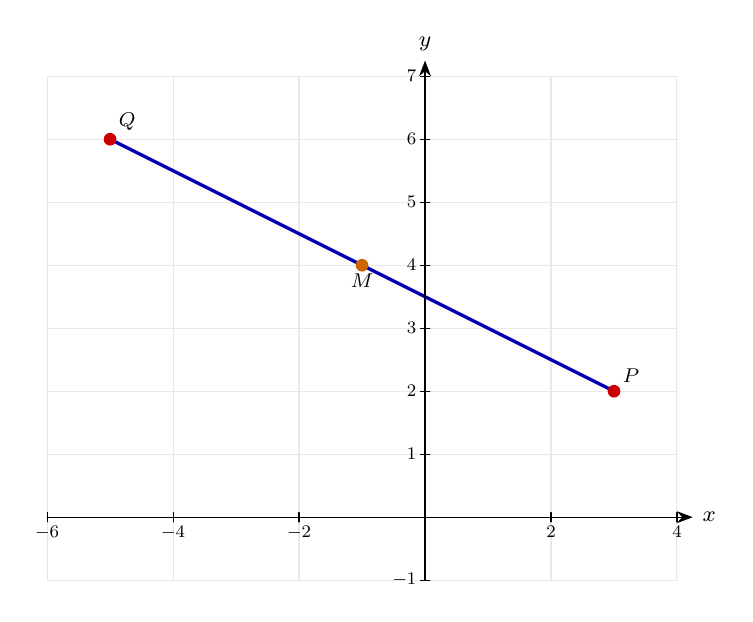
\begin{tikzpicture}[>={Stealth[length=2mm]},font=\footnotesize,line cap=round]
\begin{scope}
\clip (0,0) rectangle (8,6.4);
\draw[gray!18] (0,0) grid[xstep=1.6,ystep=0.8] (8,6.4);
\draw[blue!70!black,very thick] (7.2,2.4) -- (0.8,5.6);
\end{scope}
\draw[->] (0,0.8) -- (8.2,0.8) node[right]{$x$};
\draw[->] (4.8,0) -- (4.8,6.6) node[above]{$y$};
\draw (0,0.74) -- (0,0.86) node[below=2pt,scale=0.8]{$-6$};
\draw (1.6,0.74) -- (1.6,0.86) node[below=2pt,scale=0.8]{$-4$};
\draw (3.2,0.74) -- (3.2,0.86) node[below=2pt,scale=0.8]{$-2$};
\draw (6.4,0.74) -- (6.4,0.86) node[below=2pt,scale=0.8]{$2$};
\draw (8,0.74) -- (8,0.86) node[below=2pt,scale=0.8]{$4$};
\draw (4.74,0) -- (4.86,0) node[left=2pt,scale=0.8]{$-1$};
\draw (4.74,1.6) -- (4.86,1.6) node[left=2pt,scale=0.8]{$1$};
\draw (4.74,2.4) -- (4.86,2.4) node[left=2pt,scale=0.8]{$2$};
\draw (4.74,3.2) -- (4.86,3.2) node[left=2pt,scale=0.8]{$3$};
\draw (4.74,4) -- (4.86,4) node[left=2pt,scale=0.8]{$4$};
\draw (4.74,4.8) -- (4.86,4.8) node[left=2pt,scale=0.8]{$5$};
\draw (4.74,5.6) -- (4.86,5.6) node[left=2pt,scale=0.8]{$6$};
\draw (4.74,6.4) -- (4.86,6.4) node[left=2pt,scale=0.8]{$7$};
\fill[red!80!black] (7.2,2.4) circle (2.3pt);
\node[above right,scale=0.9] at (7.2,2.4) {$P$};
\fill[orange!80!black] (4,4) circle (2.3pt);
\node[below,scale=0.9] at (4,4) {$M$};
\fill[red!80!black] (0.8,5.6) circle (2.3pt);
\node[above right,scale=0.9] at (0.8,5.6) {$Q$};
\end{tikzpicture}
}
\end{center}
\small The points and segments shown on the coordinate plane.\normalsize

\medskip\hrule

\section*{Line Segments 11\quad\small\texttt{(cg2-011)}}
\addcontentsline{toc}{section}{Line Segments 11 (cg2-011)}
\textit{Difficulty: Foundation \quad\textbar\quad Marks: 6}

\question{Points \( A(a, 1) \) and \( B(7, b) \) both lie on the line \( y = x - 2 \). Find (i) the values of \( a \) and \( b \), (ii) the midpoint of \( AB \), and (iii) the exact length of \( AB \).}

\textbf{Worked solution.}

\textit{Step 1: (i) Substitute \( y = 1 \) into \( y = x - 2 \) to find \( a \).}
\[\begin{gathered}
1 = a - 2 \quad\quad \Rightarrow \quad\quad a = 3
\end{gathered}\]
Since \(A(a, 1)\) lies on the line, its coordinates must satisfy the equation.

\textit{Step 2: Substitute \( x = 7 \) to find \( b \).}
\[\begin{gathered}
b = 7 - 2 = 5
\end{gathered}\]
So \(A = (3, 1)\) and \(B = (7, 5)\).

\textit{Step 3: (ii) Midpoint:}
\[\begin{gathered}
M = \left(\dfrac{3 + 7}{2},\ \dfrac{1 + 5}{2}\right) = (5,\ 3)
\end{gathered}\]
Using the midpoint formula with the coordinates found in parts (i). You can verify that (5, 3) also lies on y = x - 2.

\textit{Step 4: (iii) Length:}
\[\begin{gathered}
d = \sqrt{(7 - 3)^2 + (5 - 1)^2} = \sqrt{16 + 16} = \sqrt{32} = 4\sqrt{2}
\end{gathered}\]
\(\sqrt{32} = \sqrt{16 \times 2} = 4\sqrt{2}\).

\begin{answerbox}
\textbf{Final answer:}\quad (i) \(\displaystyle a = 3,\ b = 5\); (ii) \(\displaystyle M = (5, 3)\); (iii) \(\displaystyle d = 4\sqrt{2}\)
\end{answerbox}
\textbf{Diagram.}

\begin{center}
\resizebox{\ifdim\width>\linewidth \linewidth\else \width\fi}{!}{%
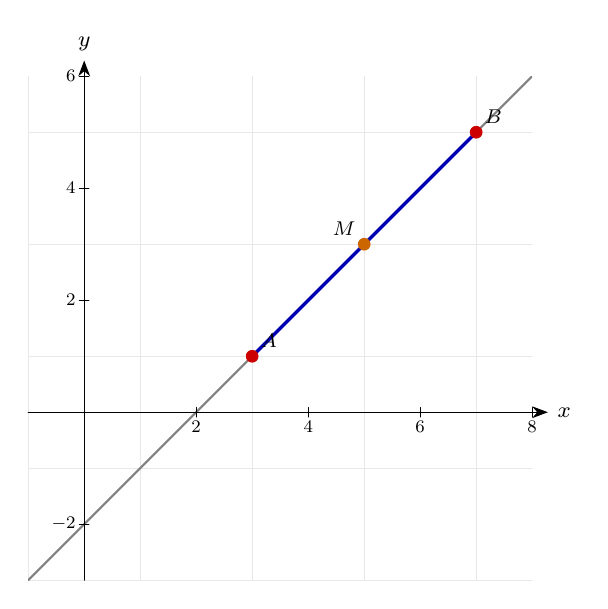
\begin{tikzpicture}[>={Stealth[length=2mm]},font=\footnotesize,line cap=round]
\begin{scope}
\clip (0,0) rectangle (6.4,6.4);
\draw[gray!18] (-0.711,-0.711) grid[xstep=1.422,ystep=1.422] (6.4,6.4);
\draw[gray,thick] (0,0) -- (6.4,6.4);
\draw[blue!70!black,very thick] (2.844,2.844) -- (5.689,5.689);
\end{scope}
\draw[->] (0,2.133) -- (6.6,2.133) node[right]{$x$};
\draw[->] (0.711,0) -- (0.711,6.6) node[above]{$y$};
\draw (2.133,2.073) -- (2.133,2.193) node[below=2pt,scale=0.8]{$2$};
\draw (3.556,2.073) -- (3.556,2.193) node[below=2pt,scale=0.8]{$4$};
\draw (4.978,2.073) -- (4.978,2.193) node[below=2pt,scale=0.8]{$6$};
\draw (6.4,2.073) -- (6.4,2.193) node[below=2pt,scale=0.8]{$8$};
\draw (0.651,0.711) -- (0.771,0.711) node[left=2pt,scale=0.8]{$-2$};
\draw (0.651,3.556) -- (0.771,3.556) node[left=2pt,scale=0.8]{$2$};
\draw (0.651,4.978) -- (0.771,4.978) node[left=2pt,scale=0.8]{$4$};
\draw (0.651,6.4) -- (0.771,6.4) node[left=2pt,scale=0.8]{$6$};
\fill[red!80!black] (2.844,2.844) circle (2.3pt);
\node[above right,scale=0.9] at (2.844,2.844) {$A$};
\fill[red!80!black] (5.689,5.689) circle (2.3pt);
\node[above right,scale=0.9] at (5.689,5.689) {$B$};
\fill[orange!80!black] (4.267,4.267) circle (2.3pt);
\node[above left,scale=0.9] at (4.267,4.267) {$M$};
\end{tikzpicture}
}
\end{center}
\small The points and segments shown on the coordinate plane.\normalsize

\medskip\hrule

\section*{Line Segments 12\quad\small\texttt{(cg2-012)}}
\addcontentsline{toc}{section}{Line Segments 12 (cg2-012)}
\textit{Difficulty: Foundation \quad\textbar\quad Marks: 6}

\question{Points \( A(a, 1) \) and \( B(b, 7) \) lie on the line \( y = 3x - 5 \). Find (i) the values of \( a \) and \( b \), (ii) the midpoint of \( AB \), (iii) the exact length of \( AB \).}

\textbf{Worked solution.}

\textit{Step 1: (i) Substitute \( y = 1 \) to find \( a \):}
\[\begin{gathered}
1 = 3a - 5 \implies 3a = 6 \implies a = 2
\end{gathered}\]
Since A(a, 1) lies on the line, substitute y = 1 and solve for x to find a.

\textit{Step 2: Substitute \( y = 7 \) to find \( b \):}
\[\begin{gathered}
7 = 3b - 5 \implies 3b = 12 \implies b = 4
\end{gathered}\]
Points: \( A = (2, 1) \), \( B = (4, 7) \).

\textit{Step 3: (ii) Midpoint:}
\[\begin{gathered}
M = \left(\dfrac{2 + 4}{2},\ \dfrac{1 + 7}{2}\right) = (3,\ 4)
\end{gathered}\]
Using the midpoint formula with the coordinates found above.

\textit{Step 4: (iii) Length:}
\[\begin{gathered}
d = \sqrt{(4 - 2)^2 + (7 - 1)^2} = \sqrt{4 + 36} = \sqrt{40} = 2\sqrt{10}
\end{gathered}\]
Simplify the surd: the largest perfect square factor of 40 is 4, so sqrt(40) = 2*sqrt(10).

\begin{answerbox}
\textbf{Final answer:}\quad (i) \(\displaystyle a = 2,\ b = 4\); (ii) \(\displaystyle M = (3, 4)\); (iii) \(\displaystyle d = 2\sqrt{10}\)
\end{answerbox}
\textbf{Diagram.}

\begin{center}
\resizebox{\ifdim\width>\linewidth \linewidth\else \width\fi}{!}{%
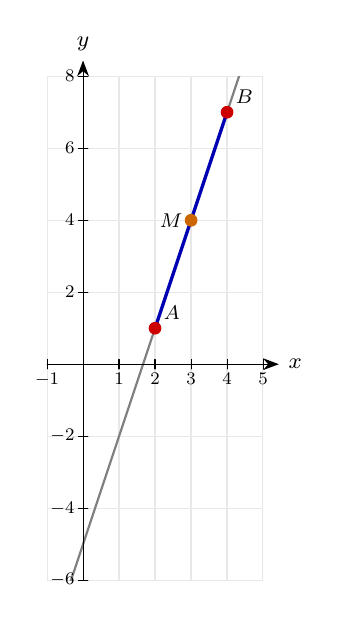
\begin{tikzpicture}[>={Stealth[length=2mm]},font=\footnotesize,line cap=round]
\begin{scope}
\clip (0,0) rectangle (2.743,6.4);
\draw[gray!18] (0,0) grid[xstep=0.457,ystep=0.914] (2.743,6.4);
\draw[gray,thick] (0,-0.914) -- (2.743,7.314);
\draw[blue!70!black,very thick] (1.371,3.2) -- (2.286,5.943);
\end{scope}
\draw[->] (0,2.743) -- (2.943,2.743) node[right]{$x$};
\draw[->] (0.457,0) -- (0.457,6.6) node[above]{$y$};
\draw (0,2.683) -- (0,2.803) node[below=2pt,scale=0.8]{$-1$};
\draw (0.914,2.683) -- (0.914,2.803) node[below=2pt,scale=0.8]{$1$};
\draw (1.371,2.683) -- (1.371,2.803) node[below=2pt,scale=0.8]{$2$};
\draw (1.829,2.683) -- (1.829,2.803) node[below=2pt,scale=0.8]{$3$};
\draw (2.286,2.683) -- (2.286,2.803) node[below=2pt,scale=0.8]{$4$};
\draw (2.743,2.683) -- (2.743,2.803) node[below=2pt,scale=0.8]{$5$};
\draw (0.397,0) -- (0.517,0) node[left=2pt,scale=0.8]{$-6$};
\draw (0.397,0.914) -- (0.517,0.914) node[left=2pt,scale=0.8]{$-4$};
\draw (0.397,1.829) -- (0.517,1.829) node[left=2pt,scale=0.8]{$-2$};
\draw (0.397,3.657) -- (0.517,3.657) node[left=2pt,scale=0.8]{$2$};
\draw (0.397,4.571) -- (0.517,4.571) node[left=2pt,scale=0.8]{$4$};
\draw (0.397,5.486) -- (0.517,5.486) node[left=2pt,scale=0.8]{$6$};
\draw (0.397,6.4) -- (0.517,6.4) node[left=2pt,scale=0.8]{$8$};
\fill[red!80!black] (1.371,3.2) circle (2.3pt);
\node[above right,scale=0.9] at (1.371,3.2) {$A$};
\fill[red!80!black] (2.286,5.943) circle (2.3pt);
\node[above right,scale=0.9] at (2.286,5.943) {$B$};
\fill[orange!80!black] (1.829,4.571) circle (2.3pt);
\node[left,scale=0.9] at (1.829,4.571) {$M$};
\end{tikzpicture}
}
\end{center}
\small The points and segments shown on the coordinate plane.\normalsize

\medskip\hrule

\section*{Line Segments 13\quad\small\texttt{(cg2-013)}}
\addcontentsline{toc}{section}{Line Segments 13 (cg2-013)}
\textit{Difficulty: Foundation \quad\textbar\quad Marks: 6}

\question{Points \( C(2, c) \) and \( D(d, 1) \) lie on the line \( y = 2x - 7 \). Find (i) the values of \( c \) and \( d \), (ii) the midpoint of \( CD \), (iii) the exact length of \( CD \).}

\textbf{Worked solution.}

\textit{Step 1: (i) Find \( c \): substitute \( x = 2 \) into \( y = 2x - 7 \).}
\[\begin{gathered}
c = 2(2) - 7 = 4 - 7 = -3
\end{gathered}\]
Since C(2, c) lies on the line, substitute x = 2 directly into y = 2x - 7 to find the y-coordinate.

\textit{Step 2: Find \( d \): substitute \( y = 1 \) into \( y = 2x - 7 \).}
\[\begin{gathered}
1 = 2d - 7 \implies 2d = 8 \implies d = 4
\end{gathered}\]
Here we know y = 1, so substitute into the equation and solve for x. This is the reverse of the previous step.

\textit{Step 3: (ii) Midpoint of \( C(2, -3) \) and \( D(4, 1) \).}
\[\begin{gathered}
M = \left(\dfrac{2 + 4}{2},\ \dfrac{-3 + 1}{2}\right) = (3,\ -1)
\end{gathered}\]
Using the midpoint formula with the coordinates found in part (i).

\textit{Step 4: (iii) Length of \( CD \).}
\[\begin{gathered}
CD = \sqrt{(4-2)^2 + (1-(-3))^2} = \sqrt{4 + 16} = \sqrt{20} = 2\sqrt{5}
\end{gathered}\]
Note that 1 - (-3) = 4. Simplify the surd: sqrt(20) = sqrt(4 * 5) = 2*sqrt(5).

\begin{answerbox}
\textbf{Final answer:}\quad (i) \(\displaystyle c = -3,\ d = 4\); (ii) \(\displaystyle M = (3, -1)\); (iii) \(\displaystyle 2\sqrt{5}\)
\end{answerbox}
\textbf{Diagram.}

\begin{center}
\resizebox{\ifdim\width>\linewidth \linewidth\else \width\fi}{!}{%
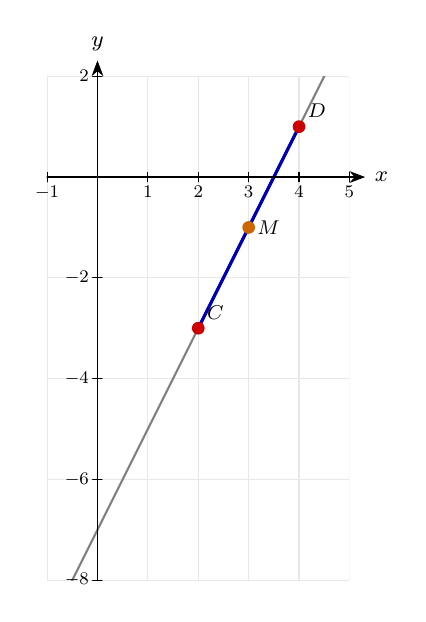
\begin{tikzpicture}[>={Stealth[length=2mm]},font=\footnotesize,line cap=round]
\begin{scope}
\clip (0,0) rectangle (3.84,6.4);
\draw[gray!18] (0,0) grid[xstep=0.64,ystep=1.28] (3.84,6.4);
\draw[gray,thick] (0,-0.64) -- (3.84,7.04);
\draw[blue!70!black,very thick] (1.92,3.2) -- (3.2,5.76);
\end{scope}
\draw[->] (0,5.12) -- (4.04,5.12) node[right]{$x$};
\draw[->] (0.64,0) -- (0.64,6.6) node[above]{$y$};
\draw (0,5.06) -- (0,5.18) node[below=2pt,scale=0.8]{$-1$};
\draw (1.28,5.06) -- (1.28,5.18) node[below=2pt,scale=0.8]{$1$};
\draw (1.92,5.06) -- (1.92,5.18) node[below=2pt,scale=0.8]{$2$};
\draw (2.56,5.06) -- (2.56,5.18) node[below=2pt,scale=0.8]{$3$};
\draw (3.2,5.06) -- (3.2,5.18) node[below=2pt,scale=0.8]{$4$};
\draw (3.84,5.06) -- (3.84,5.18) node[below=2pt,scale=0.8]{$5$};
\draw (0.58,0) -- (0.7,0) node[left=2pt,scale=0.8]{$-8$};
\draw (0.58,1.28) -- (0.7,1.28) node[left=2pt,scale=0.8]{$-6$};
\draw (0.58,2.56) -- (0.7,2.56) node[left=2pt,scale=0.8]{$-4$};
\draw (0.58,3.84) -- (0.7,3.84) node[left=2pt,scale=0.8]{$-2$};
\draw (0.58,6.4) -- (0.7,6.4) node[left=2pt,scale=0.8]{$2$};
\fill[red!80!black] (1.92,3.2) circle (2.3pt);
\node[above right,scale=0.9] at (1.92,3.2) {$C$};
\fill[red!80!black] (3.2,5.76) circle (2.3pt);
\node[above right,scale=0.9] at (3.2,5.76) {$D$};
\fill[orange!80!black] (2.56,4.48) circle (2.3pt);
\node[right,scale=0.9] at (2.56,4.48) {$M$};
\end{tikzpicture}
}
\end{center}
\small The points and segments shown on the coordinate plane.\normalsize

\medskip\hrule

\section*{Line Segments 14\quad\small\texttt{(cg2-014)}}
\addcontentsline{toc}{section}{Line Segments 14 (cg2-014)}
\textit{Difficulty: Foundation \quad\textbar\quad Marks: 7}

\question{Points \( P(p, 5) \) and \( Q(7, q) \) lie on the line \( 3x - 2y - 1 = 0 \). Find (i) \( p \) and \( q \), (ii) the midpoint of \( PQ \), (iii) the exact length of \( PQ \).}

\textbf{Worked solution.}

\textit{Step 1: (i) Substitute \( y = 5 \) to find \( p \):}
\[\begin{gathered}
3p - 10 - 1 = 0 \implies 3p = 11 \implies p = \dfrac{11}{3}
\end{gathered}\]
Substitute y = 5 into the equation 3x - 2y - 1 = 0 and solve for x. Fractional coordinates are perfectly valid.

\textit{Step 2: Substitute \( x = 7 \) to find \( q \):}
\[\begin{gathered}
21 - 2q - 1 = 0 \implies 2q = 20 \implies q = 10
\end{gathered}\]
Points: \( P = \left(\frac{11}{3}, 5\right) \), \( Q = (7, 10) \).

\textit{Step 3: (ii) Midpoint:}
\[\begin{gathered}
M = \left(\dfrac{\frac{11}{3} + 7}{2},\ \dfrac{5 + 10}{2}\right) = \left(\dfrac{\frac{32}{3}}{2},\ \dfrac{15}{2}\right) = \left(\dfrac{16}{3},\ \dfrac{15}{2}\right)
\end{gathered}\]
When averaging fractions, convert to a common denominator first: 11/3 + 7 = 11/3 + 21/3 = 32/3, then divide by 2.

\textit{Step 4: (iii) Length:}
\[\begin{gathered}
d = \sqrt{\left(7 - \tfrac{11}{3}\right)^2 + (10 - 5)^2} = \sqrt{\left(\tfrac{10}{3}\right)^2 + 25} = \sqrt{\tfrac{100}{9} + \tfrac{225}{9}} = \sqrt{\tfrac{325}{9}} = \dfrac{5\sqrt{13}}{3}
\end{gathered}\]
Convert 25 to ninths (225/9) so both terms share a denominator. Then sqrt(325) = sqrt(25 * 13) = 5*sqrt(13).

\begin{answerbox}
\textbf{Final answer:}\quad (i) \(\displaystyle p = \frac{11}{3},\ q = 10\); (ii) \(\displaystyle M = \left(\frac{16}{3}, \frac{15}{2}\right)\); (iii) \(\displaystyle \frac{5\sqrt{13}}{3}\)
\end{answerbox}
\textbf{Diagram.}

\begin{center}
\resizebox{\ifdim\width>\linewidth \linewidth\else \width\fi}{!}{%
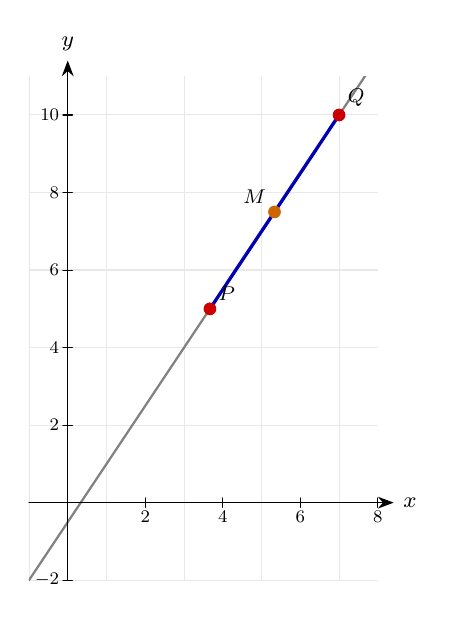
\begin{tikzpicture}[>={Stealth[length=2mm]},font=\footnotesize,line cap=round]
\begin{scope}
\clip (0,0) rectangle (4.431,6.4);
\draw[gray!18] (-0.492,0) grid[xstep=0.985,ystep=0.985] (4.431,6.4);
\draw[gray,thick] (0,0) -- (4.431,6.646);
\draw[blue!70!black,very thick] (2.298,3.446) -- (3.938,5.908);
\end{scope}
\draw[->] (0,0.985) -- (4.631,0.985) node[right]{$x$};
\draw[->] (0.492,0) -- (0.492,6.6) node[above]{$y$};
\draw (1.477,0.925) -- (1.477,1.045) node[below=2pt,scale=0.8]{$2$};
\draw (2.462,0.925) -- (2.462,1.045) node[below=2pt,scale=0.8]{$4$};
\draw (3.446,0.925) -- (3.446,1.045) node[below=2pt,scale=0.8]{$6$};
\draw (4.431,0.925) -- (4.431,1.045) node[below=2pt,scale=0.8]{$8$};
\draw (0.432,0) -- (0.552,0) node[left=2pt,scale=0.8]{$-2$};
\draw (0.432,1.969) -- (0.552,1.969) node[left=2pt,scale=0.8]{$2$};
\draw (0.432,2.954) -- (0.552,2.954) node[left=2pt,scale=0.8]{$4$};
\draw (0.432,3.938) -- (0.552,3.938) node[left=2pt,scale=0.8]{$6$};
\draw (0.432,4.923) -- (0.552,4.923) node[left=2pt,scale=0.8]{$8$};
\draw (0.432,5.908) -- (0.552,5.908) node[left=2pt,scale=0.8]{$10$};
\fill[red!80!black] (2.298,3.446) circle (2.3pt);
\node[above right,scale=0.9] at (2.298,3.446) {$P$};
\fill[red!80!black] (3.938,5.908) circle (2.3pt);
\node[above right,scale=0.9] at (3.938,5.908) {$Q$};
\fill[orange!80!black] (3.118,4.677) circle (2.3pt);
\node[above left,scale=0.9] at (3.118,4.677) {$M$};
\end{tikzpicture}
}
\end{center}
\small The points and segments shown on the coordinate plane.\normalsize

\medskip\hrule

\section*{Line Segments 15\quad\small\texttt{(cg2-015)}}
\addcontentsline{toc}{section}{Line Segments 15 (cg2-015)}
\textit{Difficulty: Foundation \quad\textbar\quad Marks: 7}

\question{The segment \( CD \) has midpoint \( (2, -1) \), gradient \( \dfrac{3}{4} \) and length \( 10 \). Find the coordinates of \( C \) and \( D \).}

\textbf{Worked solution.}

\textit{Step 1: A gradient of \( \frac{3}{4} \) means the displacement from midpoint to each end is of the form \( (4k, 3k) \) for some \( k \).}
\[\begin{gathered}
\text{Half-displacement} = (4k,\ 3k)
\end{gathered}\]
The direction vector \( (4, 3) \) has magnitude \( \sqrt{16+9}=5 \).

\textit{Step 2: The full length is \( 2 \times 5|k| = 10 \), so \( |k| = 1 \).}
\[\begin{gathered}
10|k| = 10 \implies k = 1
\end{gathered}\]
The full segment length is twice the half-length: 2 * 5|k| = 10, giving |k| = 1. We take k = 1 (choosing a direction).

\textit{Step 3: Find \( C \) and \( D \) using midpoint \( (2, -1) \) and displacement \( (4, 3) \).}
\[\begin{gathered}
C = (2 - 4,\ -1 - 3) = (-2,\ -4), \quad D = (2 + 4,\ -1 + 3) = (6,\ 2)
\end{gathered}\]
Subtract the displacement from the midpoint to get one endpoint, and add it to get the other.

\textit{Step 4: Verify length:}
\[\begin{gathered}
d = \sqrt{(6-(-2))^2 + (2-(-4))^2} = \sqrt{64+36} = \sqrt{100} = 10 \checkmark
\end{gathered}\]
Always verify your answer. The length matches the given value of 10, confirming the endpoints are correct.

\begin{answerbox}
\textbf{Final answer:}\quad \(\displaystyle C = (-2, -4)\) and \(\displaystyle D = (6, 2)\)
\end{answerbox}
\textbf{Diagram.}

\begin{center}
\resizebox{\ifdim\width>\linewidth \linewidth\else \width\fi}{!}{%
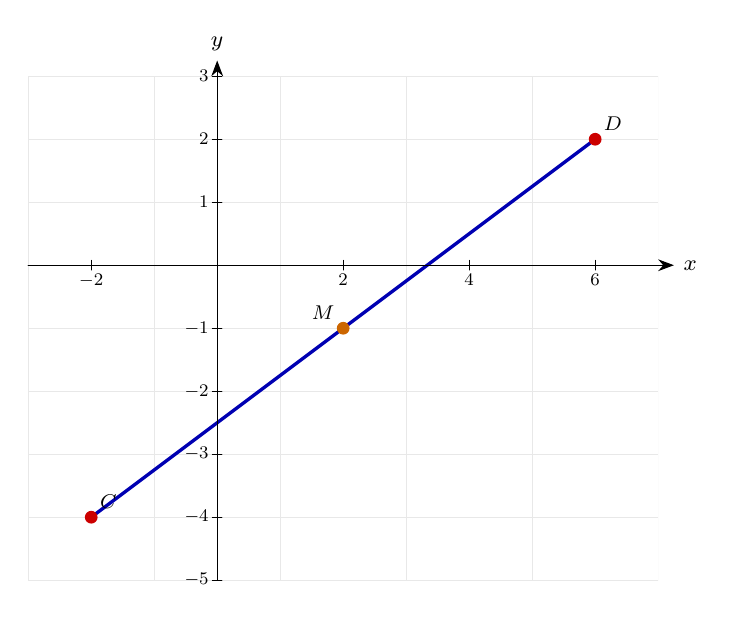
\begin{tikzpicture}[>={Stealth[length=2mm]},font=\footnotesize,line cap=round]
\begin{scope}
\clip (0,0) rectangle (8,6.4);
\draw[gray!18] (-0.8,0) grid[xstep=1.6,ystep=0.8] (8,6.4);
\draw[blue!70!black,very thick] (0.8,0.8) -- (7.2,5.6);
\end{scope}
\draw[->] (0,4) -- (8.2,4) node[right]{$x$};
\draw[->] (2.4,0) -- (2.4,6.6) node[above]{$y$};
\draw (0.8,3.94) -- (0.8,4.06) node[below=2pt,scale=0.8]{$-2$};
\draw (4,3.94) -- (4,4.06) node[below=2pt,scale=0.8]{$2$};
\draw (5.6,3.94) -- (5.6,4.06) node[below=2pt,scale=0.8]{$4$};
\draw (7.2,3.94) -- (7.2,4.06) node[below=2pt,scale=0.8]{$6$};
\draw (2.34,0) -- (2.46,0) node[left=2pt,scale=0.8]{$-5$};
\draw (2.34,0.8) -- (2.46,0.8) node[left=2pt,scale=0.8]{$-4$};
\draw (2.34,1.6) -- (2.46,1.6) node[left=2pt,scale=0.8]{$-3$};
\draw (2.34,2.4) -- (2.46,2.4) node[left=2pt,scale=0.8]{$-2$};
\draw (2.34,3.2) -- (2.46,3.2) node[left=2pt,scale=0.8]{$-1$};
\draw (2.34,4.8) -- (2.46,4.8) node[left=2pt,scale=0.8]{$1$};
\draw (2.34,5.6) -- (2.46,5.6) node[left=2pt,scale=0.8]{$2$};
\draw (2.34,6.4) -- (2.46,6.4) node[left=2pt,scale=0.8]{$3$};
\fill[red!80!black] (0.8,0.8) circle (2.3pt);
\node[above right,scale=0.9] at (0.8,0.8) {$C$};
\fill[red!80!black] (7.2,5.6) circle (2.3pt);
\node[above right,scale=0.9] at (7.2,5.6) {$D$};
\fill[orange!80!black] (4,3.2) circle (2.3pt);
\node[above left,scale=0.9] at (4,3.2) {$M$};
\end{tikzpicture}
}
\end{center}
\small The points and segments shown on the coordinate plane.\normalsize

\medskip\hrule

\section*{Line Segments 16\quad\small\texttt{(cg2-016)}}
\addcontentsline{toc}{section}{Line Segments 16 (cg2-016)}
\textit{Difficulty: Foundation \quad\textbar\quad Marks: 2}

\question{Find the midpoint of \( A(-3, 8) \) and \( B(5, -2) \).}

\textbf{Worked solution.}

\textit{Apply midpoint formula}
\[\begin{gathered}
M = \left(\frac{-3+5}{2}, \frac{8+(-2)}{2}\right) = (1, 3)
\end{gathered}\]
Average each coordinate.

\begin{answerbox}
\textbf{Final answer:}\quad \(\displaystyle (1, 3)\)
\end{answerbox}
\textbf{Diagram.}

\begin{center}
\resizebox{\ifdim\width>\linewidth \linewidth\else \width\fi}{!}{%
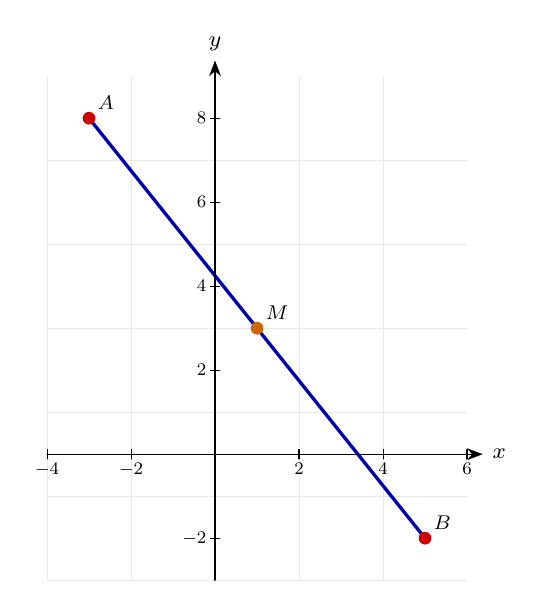
\begin{tikzpicture}[>={Stealth[length=2mm]},font=\footnotesize,line cap=round]
\begin{scope}
\clip (0,0) rectangle (5.333,6.4);
\draw[gray!18] (0,-0.533) grid[xstep=1.067,ystep=1.067] (5.333,6.4);
\draw[blue!70!black,very thick] (0.533,5.867) -- (4.8,0.533);
\end{scope}
\draw[->] (0,1.6) -- (5.533,1.6) node[right]{$x$};
\draw[->] (2.133,0) -- (2.133,6.6) node[above]{$y$};
\draw (0,1.54) -- (0,1.66) node[below=2pt,scale=0.8]{$-4$};
\draw (1.067,1.54) -- (1.067,1.66) node[below=2pt,scale=0.8]{$-2$};
\draw (3.2,1.54) -- (3.2,1.66) node[below=2pt,scale=0.8]{$2$};
\draw (4.267,1.54) -- (4.267,1.66) node[below=2pt,scale=0.8]{$4$};
\draw (5.333,1.54) -- (5.333,1.66) node[below=2pt,scale=0.8]{$6$};
\draw (2.073,0.533) -- (2.193,0.533) node[left=2pt,scale=0.8]{$-2$};
\draw (2.073,2.667) -- (2.193,2.667) node[left=2pt,scale=0.8]{$2$};
\draw (2.073,3.733) -- (2.193,3.733) node[left=2pt,scale=0.8]{$4$};
\draw (2.073,4.8) -- (2.193,4.8) node[left=2pt,scale=0.8]{$6$};
\draw (2.073,5.867) -- (2.193,5.867) node[left=2pt,scale=0.8]{$8$};
\fill[red!80!black] (0.533,5.867) circle (2.3pt);
\node[above right,scale=0.9] at (0.533,5.867) {$A$};
\fill[red!80!black] (4.8,0.533) circle (2.3pt);
\node[above right,scale=0.9] at (4.8,0.533) {$B$};
\fill[orange!80!black] (2.667,3.2) circle (2.3pt);
\node[above right,scale=0.9] at (2.667,3.2) {$M$};
\end{tikzpicture}
}
\end{center}
\small The points and segments shown on the coordinate plane.\normalsize

\medskip\hrule

\section*{Line Segments 17\quad\small\texttt{(cg2-017)}}
\addcontentsline{toc}{section}{Line Segments 17 (cg2-017)}
\textit{Difficulty: Foundation \quad\textbar\quad Marks: 2}

\question{Find the distance between \( P(-1, 4) \) and \( Q(5, -4) \).}

\textbf{Worked solution.}

\textit{Distance formula}
\[\begin{gathered}
PQ = \sqrt{(5-(-1))^2 + (-4-4)^2} = \sqrt{36 + 64} = \sqrt{100} = 10
\end{gathered}\]
Using the distance formula. Be careful: 5 - (-1) = 6, not 4. This is a 6-8-10 Pythagorean triple.

\begin{answerbox}
\textbf{Final answer:}\quad \(\displaystyle 10\)
\end{answerbox}
\textbf{Diagram.}

\begin{center}
\resizebox{\ifdim\width>\linewidth \linewidth\else \width\fi}{!}{%
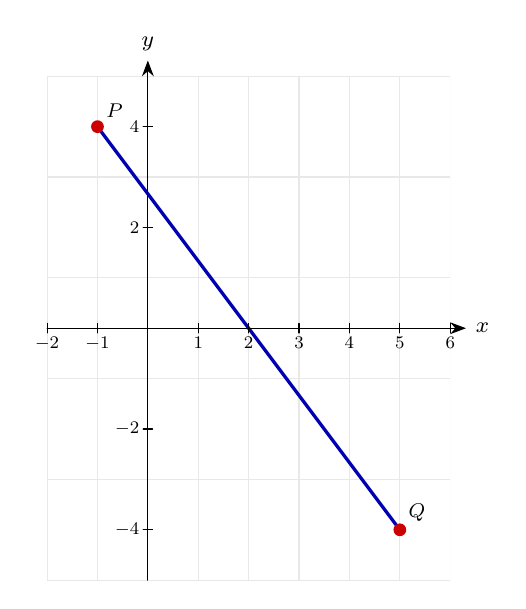
\begin{tikzpicture}[>={Stealth[length=2mm]},font=\footnotesize,line cap=round]
\begin{scope}
\clip (0,0) rectangle (5.12,6.4);
\draw[gray!18] (0,-0.64) grid[xstep=0.64,ystep=1.28] (5.12,6.4);
\draw[blue!70!black,very thick] (0.64,5.76) -- (4.48,0.64);
\end{scope}
\draw[->] (0,3.2) -- (5.32,3.2) node[right]{$x$};
\draw[->] (1.28,0) -- (1.28,6.6) node[above]{$y$};
\draw (0,3.14) -- (0,3.26) node[below=2pt,scale=0.8]{$-2$};
\draw (0.64,3.14) -- (0.64,3.26) node[below=2pt,scale=0.8]{$-1$};
\draw (1.92,3.14) -- (1.92,3.26) node[below=2pt,scale=0.8]{$1$};
\draw (2.56,3.14) -- (2.56,3.26) node[below=2pt,scale=0.8]{$2$};
\draw (3.2,3.14) -- (3.2,3.26) node[below=2pt,scale=0.8]{$3$};
\draw (3.84,3.14) -- (3.84,3.26) node[below=2pt,scale=0.8]{$4$};
\draw (4.48,3.14) -- (4.48,3.26) node[below=2pt,scale=0.8]{$5$};
\draw (5.12,3.14) -- (5.12,3.26) node[below=2pt,scale=0.8]{$6$};
\draw (1.22,0.64) -- (1.34,0.64) node[left=2pt,scale=0.8]{$-4$};
\draw (1.22,1.92) -- (1.34,1.92) node[left=2pt,scale=0.8]{$-2$};
\draw (1.22,4.48) -- (1.34,4.48) node[left=2pt,scale=0.8]{$2$};
\draw (1.22,5.76) -- (1.34,5.76) node[left=2pt,scale=0.8]{$4$};
\fill[red!80!black] (0.64,5.76) circle (2.3pt);
\node[above right,scale=0.9] at (0.64,5.76) {$P$};
\fill[red!80!black] (4.48,0.64) circle (2.3pt);
\node[above right,scale=0.9] at (4.48,0.64) {$Q$};
\end{tikzpicture}
}
\end{center}
\small The points and segments shown on the coordinate plane.\normalsize

\medskip\hrule

\section*{Line Segments 18\quad\small\texttt{(cg2-018)}}
\addcontentsline{toc}{section}{Line Segments 18 (cg2-018)}
\textit{Difficulty: Foundation \quad\textbar\quad Marks: 2}

\question{The midpoint of \( A(2, k) \) and \( B(8, 3) \) is \( (5, 7) \). Find \( k \).}

\textbf{Worked solution.}

\textit{Use midpoint y-coordinate}
\[\begin{gathered}
\frac{k + 3}{2} = 7 \implies k + 3 = 14 \implies k = 11
\end{gathered}\]
Set the y-component of the midpoint formula equal to 7 and solve. Multiply both sides by 2 first to clear the fraction.

\begin{answerbox}
\textbf{Final answer:}\quad \(\displaystyle k = 11\)
\end{answerbox}
\textbf{Diagram.}

\begin{center}
\resizebox{\ifdim\width>\linewidth \linewidth\else \width\fi}{!}{%
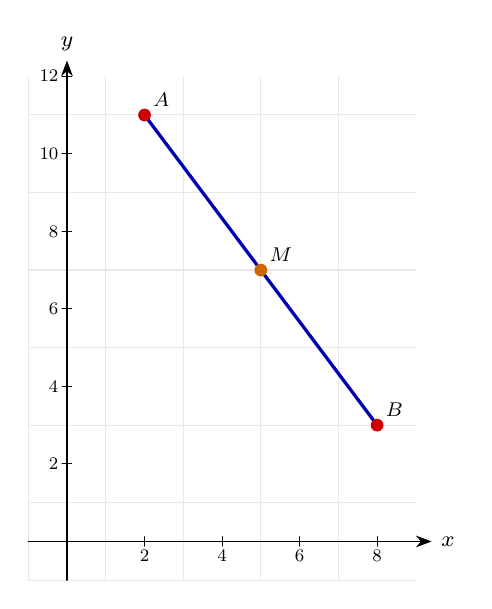
\begin{tikzpicture}[>={Stealth[length=2mm]},font=\footnotesize,line cap=round]
\begin{scope}
\clip (0,0) rectangle (4.923,6.4);
\draw[gray!18] (-0.492,-0.492) grid[xstep=0.985,ystep=0.985] (4.923,6.4);
\draw[blue!70!black,very thick] (1.477,5.908) -- (4.431,1.969);
\end{scope}
\draw[->] (0,0.492) -- (5.123,0.492) node[right]{$x$};
\draw[->] (0.492,0) -- (0.492,6.6) node[above]{$y$};
\draw (1.477,0.432) -- (1.477,0.552) node[below=2pt,scale=0.8]{$2$};
\draw (2.462,0.432) -- (2.462,0.552) node[below=2pt,scale=0.8]{$4$};
\draw (3.446,0.432) -- (3.446,0.552) node[below=2pt,scale=0.8]{$6$};
\draw (4.431,0.432) -- (4.431,0.552) node[below=2pt,scale=0.8]{$8$};
\draw (0.432,1.477) -- (0.552,1.477) node[left=2pt,scale=0.8]{$2$};
\draw (0.432,2.462) -- (0.552,2.462) node[left=2pt,scale=0.8]{$4$};
\draw (0.432,3.446) -- (0.552,3.446) node[left=2pt,scale=0.8]{$6$};
\draw (0.432,4.431) -- (0.552,4.431) node[left=2pt,scale=0.8]{$8$};
\draw (0.432,5.415) -- (0.552,5.415) node[left=2pt,scale=0.8]{$10$};
\draw (0.432,6.4) -- (0.552,6.4) node[left=2pt,scale=0.8]{$12$};
\fill[red!80!black] (1.477,5.908) circle (2.3pt);
\node[above right,scale=0.9] at (1.477,5.908) {$A$};
\fill[red!80!black] (4.431,1.969) circle (2.3pt);
\node[above right,scale=0.9] at (4.431,1.969) {$B$};
\fill[orange!80!black] (2.954,3.938) circle (2.3pt);
\node[above right,scale=0.9] at (2.954,3.938) {$M$};
\end{tikzpicture}
}
\end{center}
\small The points and segments shown on the coordinate plane.\normalsize

\medskip\hrule

\section*{Line Segments 19\quad\small\texttt{(cg2-019)}}
\addcontentsline{toc}{section}{Line Segments 19 (cg2-019)}
\textit{Difficulty: Foundation \quad\textbar\quad Marks: 2}

\question{Find the length of the line segment from \( (0, 0) \) to \( (7, 24) \).}

\textbf{Worked solution.}

\textit{Distance formula}
\[\begin{gathered}
d = \sqrt{49 + 576} = \sqrt{625} = 25
\end{gathered}\]
This is a 7-24-25 Pythagorean triple. When one endpoint is the origin, the formula simplifies to sqrt(x\textasciicircum 2 + y\textasciicircum 2).

\begin{answerbox}
\textbf{Final answer:}\quad \(\displaystyle 25\)
\end{answerbox}
\textbf{Diagram.}

\begin{center}
\resizebox{\ifdim\width>\linewidth \linewidth\else \width\fi}{!}{%
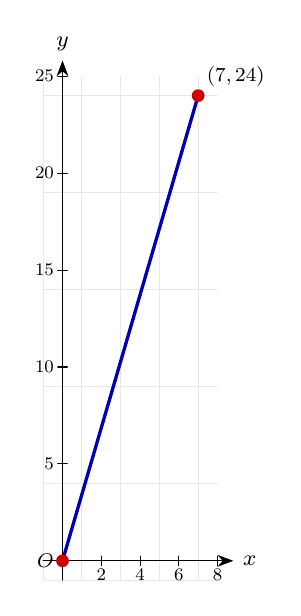
\begin{tikzpicture}[>={Stealth[length=2mm]},font=\footnotesize,line cap=round]
\begin{scope}
\clip (0,0) rectangle (2.215,6.4);
\draw[gray!18] (-0.246,-0.985) grid[xstep=0.492,ystep=1.231] (2.215,6.4);
\draw[blue!70!black,very thick] (0.246,0.246) -- (1.969,6.154);
\end{scope}
\draw[->] (0,0.246) -- (2.415,0.246) node[right]{$x$};
\draw[->] (0.246,0) -- (0.246,6.6) node[above]{$y$};
\draw (0.738,0.186) -- (0.738,0.306) node[below=2pt,scale=0.8]{$2$};
\draw (1.231,0.186) -- (1.231,0.306) node[below=2pt,scale=0.8]{$4$};
\draw (1.723,0.186) -- (1.723,0.306) node[below=2pt,scale=0.8]{$6$};
\draw (2.215,0.186) -- (2.215,0.306) node[below=2pt,scale=0.8]{$8$};
\draw (0.186,1.477) -- (0.306,1.477) node[left=2pt,scale=0.8]{$5$};
\draw (0.186,2.708) -- (0.306,2.708) node[left=2pt,scale=0.8]{$10$};
\draw (0.186,3.938) -- (0.306,3.938) node[left=2pt,scale=0.8]{$15$};
\draw (0.186,5.169) -- (0.306,5.169) node[left=2pt,scale=0.8]{$20$};
\draw (0.186,6.4) -- (0.306,6.4) node[left=2pt,scale=0.8]{$25$};
\fill[red!80!black] (0.246,0.246) circle (2.3pt);
\node[left,scale=0.9] at (0.246,0.246) {$O$};
\fill[red!80!black] (1.969,6.154) circle (2.3pt);
\node[above right,scale=0.9] at (1.969,6.154) {$(7,24)$};
\end{tikzpicture}
}
\end{center}
\small The points and segments shown on the coordinate plane.\normalsize

\medskip\hrule

\section*{Line Segments 20\quad\small\texttt{(cg2-020)}}
\addcontentsline{toc}{section}{Line Segments 20 (cg2-020)}
\textit{Difficulty: Foundation \quad\textbar\quad Marks: 3}

\question{The midpoint of \( PQ \) is \( (3, -1) \). If \( P = (7, 5) \), find \( Q \).}

\textbf{Worked solution.}

\textit{Use midpoint formula backwards}
\[\begin{gathered}
\frac{7 + x}{2} = 3 \implies x = -1; \quad \frac{5 + y}{2} = -1 \implies y = -7
\end{gathered}\]
Rearranging the midpoint formula for each coordinate: set (x\_P + x\_Q)/2 equal to the midpoint coordinate and solve for the unknown.

\begin{answerbox}
\textbf{Final answer:}\quad \(\displaystyle Q = (-1, -7)\)
\end{answerbox}
\textbf{Diagram.}

\begin{center}
\resizebox{\ifdim\width>\linewidth \linewidth\else \width\fi}{!}{%
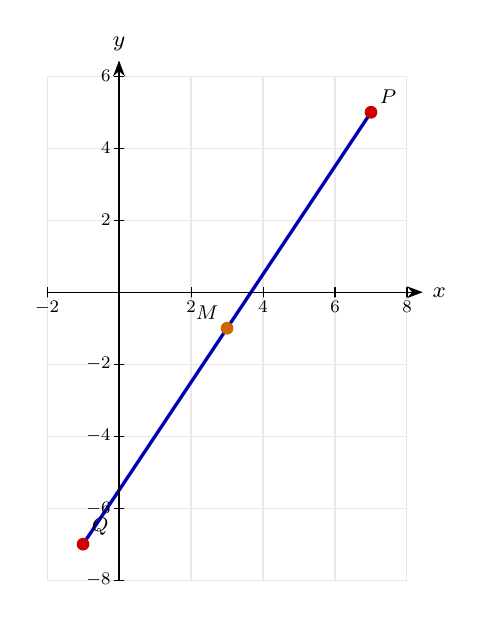
\begin{tikzpicture}[>={Stealth[length=2mm]},font=\footnotesize,line cap=round]
\begin{scope}
\clip (0,0) rectangle (4.571,6.4);
\draw[gray!18] (0,0) grid[xstep=0.914,ystep=0.914] (4.571,6.4);
\draw[blue!70!black,very thick] (4.114,5.943) -- (0.457,0.457);
\end{scope}
\draw[->] (0,3.657) -- (4.771,3.657) node[right]{$x$};
\draw[->] (0.914,0) -- (0.914,6.6) node[above]{$y$};
\draw (0,3.597) -- (0,3.717) node[below=2pt,scale=0.8]{$-2$};
\draw (1.829,3.597) -- (1.829,3.717) node[below=2pt,scale=0.8]{$2$};
\draw (2.743,3.597) -- (2.743,3.717) node[below=2pt,scale=0.8]{$4$};
\draw (3.657,3.597) -- (3.657,3.717) node[below=2pt,scale=0.8]{$6$};
\draw (4.571,3.597) -- (4.571,3.717) node[below=2pt,scale=0.8]{$8$};
\draw (0.854,0) -- (0.974,0) node[left=2pt,scale=0.8]{$-8$};
\draw (0.854,0.914) -- (0.974,0.914) node[left=2pt,scale=0.8]{$-6$};
\draw (0.854,1.829) -- (0.974,1.829) node[left=2pt,scale=0.8]{$-4$};
\draw (0.854,2.743) -- (0.974,2.743) node[left=2pt,scale=0.8]{$-2$};
\draw (0.854,4.571) -- (0.974,4.571) node[left=2pt,scale=0.8]{$2$};
\draw (0.854,5.486) -- (0.974,5.486) node[left=2pt,scale=0.8]{$4$};
\draw (0.854,6.4) -- (0.974,6.4) node[left=2pt,scale=0.8]{$6$};
\fill[red!80!black] (4.114,5.943) circle (2.3pt);
\node[above right,scale=0.9] at (4.114,5.943) {$P$};
\fill[red!80!black] (0.457,0.457) circle (2.3pt);
\node[above right,scale=0.9] at (0.457,0.457) {$Q$};
\fill[orange!80!black] (2.286,3.2) circle (2.3pt);
\node[above left,scale=0.9] at (2.286,3.2) {$M$};
\end{tikzpicture}
}
\end{center}
\small The points and segments shown on the coordinate plane.\normalsize

\medskip\hrule

\section*{Line Segments 21\quad\small\texttt{(cg2-021)}}
\addcontentsline{toc}{section}{Line Segments 21 (cg2-021)}
\textit{Difficulty: Foundation \quad\textbar\quad Marks: 3}

\question{Show that the triangle with vertices \( A(1, 1) \), \( B(5, 1) \), \( C(3, 5) \) is isosceles.}

\textbf{Worked solution.}

\textit{Find lengths}
\[\begin{gathered}
AB = 4, \quad AC = \sqrt{4+16} = \sqrt{20}, \quad BC = \sqrt{4+16} = \sqrt{20}
\end{gathered}\]
AC = BC so the triangle is isosceles.

\begin{answerbox}
\textbf{Final answer:}\quad \(\displaystyle AC = BC = \sqrt{20}\), so triangle is isosceles.
\end{answerbox}
\textbf{Diagram.}

\begin{center}
\resizebox{\ifdim\width>\linewidth \linewidth\else \width\fi}{!}{%
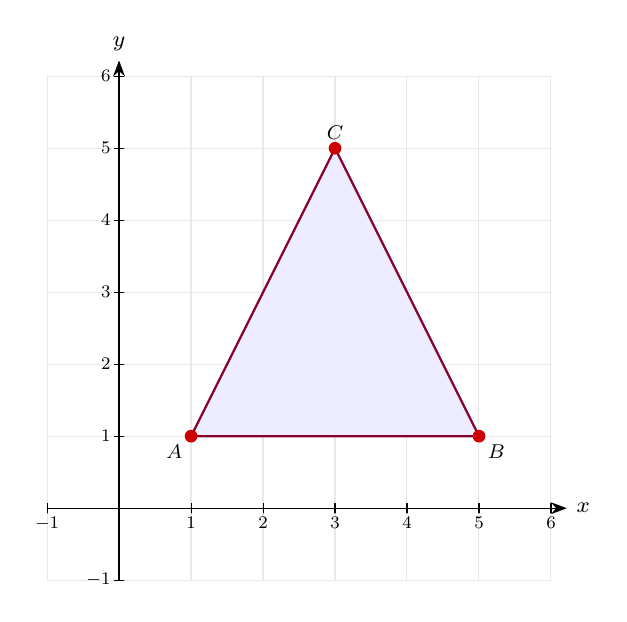
\begin{tikzpicture}[>={Stealth[length=2mm]},font=\footnotesize,line cap=round]
\begin{scope}
\clip (0,0) rectangle (6.4,6.4);
\draw[gray!18] (0,0) grid[xstep=0.914,ystep=0.914] (6.4,6.4);
\fill[blue!7] (1.829,1.829) -- (5.486,1.829) -- (3.657,5.486) -- cycle;
\draw[purple!70!black,thick] (1.829,1.829) -- (5.486,1.829) -- (3.657,5.486) -- cycle;
\end{scope}
\draw[->] (0,0.914) -- (6.6,0.914) node[right]{$x$};
\draw[->] (0.914,0) -- (0.914,6.6) node[above]{$y$};
\draw (0,0.854) -- (0,0.974) node[below=2pt,scale=0.8]{$-1$};
\draw (1.829,0.854) -- (1.829,0.974) node[below=2pt,scale=0.8]{$1$};
\draw (2.743,0.854) -- (2.743,0.974) node[below=2pt,scale=0.8]{$2$};
\draw (3.657,0.854) -- (3.657,0.974) node[below=2pt,scale=0.8]{$3$};
\draw (4.571,0.854) -- (4.571,0.974) node[below=2pt,scale=0.8]{$4$};
\draw (5.486,0.854) -- (5.486,0.974) node[below=2pt,scale=0.8]{$5$};
\draw (6.4,0.854) -- (6.4,0.974) node[below=2pt,scale=0.8]{$6$};
\draw (0.854,0) -- (0.974,0) node[left=2pt,scale=0.8]{$-1$};
\draw (0.854,1.829) -- (0.974,1.829) node[left=2pt,scale=0.8]{$1$};
\draw (0.854,2.743) -- (0.974,2.743) node[left=2pt,scale=0.8]{$2$};
\draw (0.854,3.657) -- (0.974,3.657) node[left=2pt,scale=0.8]{$3$};
\draw (0.854,4.571) -- (0.974,4.571) node[left=2pt,scale=0.8]{$4$};
\draw (0.854,5.486) -- (0.974,5.486) node[left=2pt,scale=0.8]{$5$};
\draw (0.854,6.4) -- (0.974,6.4) node[left=2pt,scale=0.8]{$6$};
\fill[red!80!black] (1.829,1.829) circle (2.3pt);
\node[below left,scale=0.9] at (1.829,1.829) {$A$};
\fill[red!80!black] (5.486,1.829) circle (2.3pt);
\node[below right,scale=0.9] at (5.486,1.829) {$B$};
\fill[red!80!black] (3.657,5.486) circle (2.3pt);
\node[above,scale=0.9] at (3.657,5.486) {$C$};
\end{tikzpicture}
}
\end{center}
\small The points and segments shown on the coordinate plane.\normalsize

\medskip\hrule

\section*{Line Segments 22\quad\small\texttt{(cg2-022)}}
\addcontentsline{toc}{section}{Line Segments 22 (cg2-022)}
\textit{Difficulty: Foundation \quad\textbar\quad Marks: 3}

\question{Find the point that divides the line segment from \( A(1, 2) \) to \( B(7, 8) \) in the ratio \( 1:2 \).}

\textbf{Worked solution.}

\textit{Step 1: Recall the section formula.}
\[\begin{gathered}
\text{If } P \text{ divides } AB \text{ in the ratio } m:n, \text{ then } P = \left(\frac{mx_2 + nx_1}{m+n},\ \frac{my_2 + ny_1}{m+n}\right)
\end{gathered}\]
The point P is closer to A since the ratio is 1:2, meaning P is one-third of the way from A to B.

\textit{Step 2: Identify the values: \( A(1,2) \), \( B(7,8) \), \( m = 1 \), \( n = 2 \).}
\[\begin{gathered}
x_1 = 1,\quad y_1 = 2,\quad x_2 = 7,\quad y_2 = 8
\end{gathered}\]
A is the first point and B is the second point. The ratio 1:2 means m = 1 (towards B) and n = 2 (towards A).

\textit{Step 3: Calculate the x-coordinate of P.}
\[\begin{gathered}
x_P = \frac{1(7) + 2(1)}{1 + 2} = \frac{7 + 2}{3} = \frac{9}{3} = 3
\end{gathered}\]
Multiply x by m and x by n, then divide by (m + n).

\textit{Step 4: Calculate the y-coordinate of P.}
\[\begin{gathered}
y_P = \frac{1(8) + 2(2)}{1 + 2} = \frac{8 + 4}{3} = \frac{12}{3} = 4
\end{gathered}\]
Multiply y by m and y by n, then divide by (m + n).

\textit{Step 5: State the answer.}
\[\begin{gathered}
P = (3,\ 4)
\end{gathered}\]
We can verify: from A(1,2) to P(3,4) the change is (+2, +2), and from P(3,4) to B(7,8) the change is (+4, +4). The ratio of these changes is 2:4 = 1:2, confirming our answer.

\begin{answerbox}
\textbf{Final answer:}\quad \(\displaystyle P = (3,\ 4)\)
\end{answerbox}
\textbf{Diagram.}

\begin{center}
\resizebox{\ifdim\width>\linewidth \linewidth\else \width\fi}{!}{%
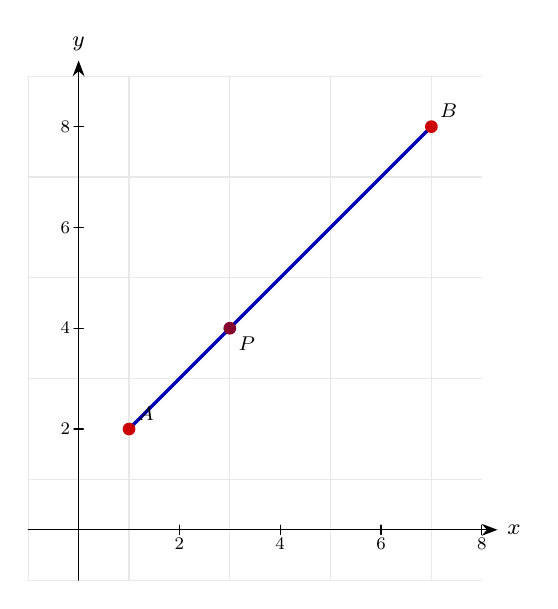
\begin{tikzpicture}[>={Stealth[length=2mm]},font=\footnotesize,line cap=round]
\begin{scope}
\clip (0,0) rectangle (5.76,6.4);
\draw[gray!18] (-0.64,-0.64) grid[xstep=1.28,ystep=1.28] (5.76,6.4);
\draw[blue!70!black,very thick] (1.28,1.92) -- (5.12,5.76);
\end{scope}
\draw[->] (0,0.64) -- (5.96,0.64) node[right]{$x$};
\draw[->] (0.64,0) -- (0.64,6.6) node[above]{$y$};
\draw (1.92,0.58) -- (1.92,0.7) node[below=2pt,scale=0.8]{$2$};
\draw (3.2,0.58) -- (3.2,0.7) node[below=2pt,scale=0.8]{$4$};
\draw (4.48,0.58) -- (4.48,0.7) node[below=2pt,scale=0.8]{$6$};
\draw (5.76,0.58) -- (5.76,0.7) node[below=2pt,scale=0.8]{$8$};
\draw (0.58,1.92) -- (0.7,1.92) node[left=2pt,scale=0.8]{$2$};
\draw (0.58,3.2) -- (0.7,3.2) node[left=2pt,scale=0.8]{$4$};
\draw (0.58,4.48) -- (0.7,4.48) node[left=2pt,scale=0.8]{$6$};
\draw (0.58,5.76) -- (0.7,5.76) node[left=2pt,scale=0.8]{$8$};
\fill[red!80!black] (1.28,1.92) circle (2.3pt);
\node[above right,scale=0.9] at (1.28,1.92) {$A$};
\fill[red!80!black] (5.12,5.76) circle (2.3pt);
\node[above right,scale=0.9] at (5.12,5.76) {$B$};
\fill[purple!70!black] (2.56,3.2) circle (2.3pt);
\node[below right,scale=0.9] at (2.56,3.2) {$P$};
\end{tikzpicture}
}
\end{center}
\small The points and segments shown on the coordinate plane.\normalsize

\medskip\hrule

\section*{Line Segments 23\quad\small\texttt{(cg2-023)}}
\addcontentsline{toc}{section}{Line Segments 23 (cg2-023)}
\textit{Difficulty: Foundation \quad\textbar\quad Marks: 3}

\question{Find the distance between \( (-3, -5) \) and \( (9, 11) \). Give your answer as a surd in simplest form.}

\textbf{Worked solution.}

\textit{Distance formula}
\[\begin{gathered}
d = \sqrt{12^2 + 16^2} = \sqrt{144+256} = \sqrt{400} = 20
\end{gathered}\]
The differences are 9 - (-3) = 12 and 11 - (-5) = 16. This is a 12-16-20 triple (a multiple of 3-4-5).

\begin{answerbox}
\textbf{Final answer:}\quad \(\displaystyle 20\)
\end{answerbox}
\textbf{Diagram.}

\begin{center}
\resizebox{\ifdim\width>\linewidth \linewidth\else \width\fi}{!}{%
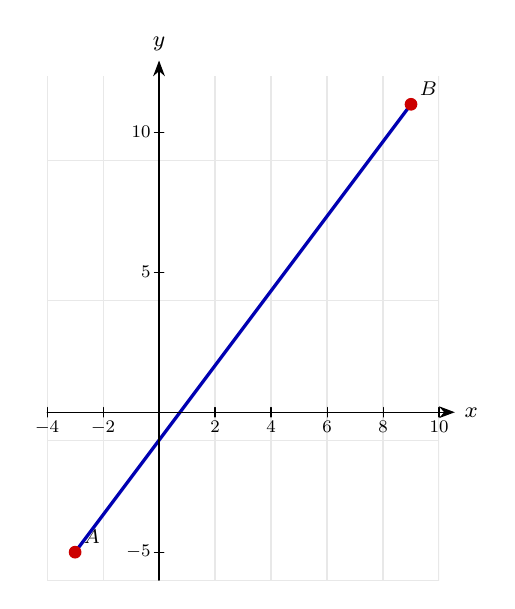
\begin{tikzpicture}[>={Stealth[length=2mm]},font=\footnotesize,line cap=round]
\begin{scope}
\clip (0,0) rectangle (4.978,6.4);
\draw[gray!18] (0,-1.422) grid[xstep=0.711,ystep=1.778] (4.978,6.4);
\draw[blue!70!black,very thick] (0.356,0.356) -- (4.622,6.044);
\end{scope}
\draw[->] (0,2.133) -- (5.178,2.133) node[right]{$x$};
\draw[->] (1.422,0) -- (1.422,6.6) node[above]{$y$};
\draw (0,2.073) -- (0,2.193) node[below=2pt,scale=0.8]{$-4$};
\draw (0.711,2.073) -- (0.711,2.193) node[below=2pt,scale=0.8]{$-2$};
\draw (2.133,2.073) -- (2.133,2.193) node[below=2pt,scale=0.8]{$2$};
\draw (2.844,2.073) -- (2.844,2.193) node[below=2pt,scale=0.8]{$4$};
\draw (3.556,2.073) -- (3.556,2.193) node[below=2pt,scale=0.8]{$6$};
\draw (4.267,2.073) -- (4.267,2.193) node[below=2pt,scale=0.8]{$8$};
\draw (4.978,2.073) -- (4.978,2.193) node[below=2pt,scale=0.8]{$10$};
\draw (1.362,0.356) -- (1.482,0.356) node[left=2pt,scale=0.8]{$-5$};
\draw (1.362,3.911) -- (1.482,3.911) node[left=2pt,scale=0.8]{$5$};
\draw (1.362,5.689) -- (1.482,5.689) node[left=2pt,scale=0.8]{$10$};
\fill[red!80!black] (0.356,0.356) circle (2.3pt);
\node[above right,scale=0.9] at (0.356,0.356) {$A$};
\fill[red!80!black] (4.622,6.044) circle (2.3pt);
\node[above right,scale=0.9] at (4.622,6.044) {$B$};
\end{tikzpicture}
}
\end{center}
\small The points and segments shown on the coordinate plane.\normalsize

\medskip\hrule

\section*{Line Segments 24\quad\small\texttt{(cg2-024)}}
\addcontentsline{toc}{section}{Line Segments 24 (cg2-024)}
\textit{Difficulty: Foundation \quad\textbar\quad Marks: 4}

\question{The points \( A(a, 3) \) and \( B(5, a) \) are such that \( AB = 5 \). Find the possible values of \( a \).}

\textbf{Worked solution.}

\textit{Step 1: Set up distance equation}
\[\begin{gathered}
(5-a)^2 + (a-3)^2 = 25
\end{gathered}\]
Apply the distance formula and square both sides to eliminate the square root, since AB = 5 means AB\textasciicircum 2 = 25.

\textit{Step 2: Expand and simplify}
\[\begin{gathered}
25 - 10a + a^2 + a^2 - 6a + 9 = 25 \implies 2a^2 - 16a + 9 = 0
\end{gathered}\]
Expand each squared bracket carefully and collect like terms. The 25 on each side cancels.

\textit{Step 3: Solve using quadratic formula}
\[\begin{gathered}
a = \frac{16 \pm \sqrt{256-72}}{4} = \frac{16 \pm \sqrt{184}}{4} = 4 \pm \frac{\sqrt{46}}{2}
\end{gathered}\]
Apply the quadratic formula with a=2, b=-16, c=9. Two solutions exist because there are two points at distance 5 from B(5,a) with y-coordinate 3.

\begin{answerbox}
\textbf{Final answer:}\quad \(\displaystyle a = 4 \pm \frac{\sqrt{46}}{2}\)
\end{answerbox}
\textbf{Diagram.}

\begin{center}
\resizebox{\ifdim\width>\linewidth \linewidth\else \width\fi}{!}{%
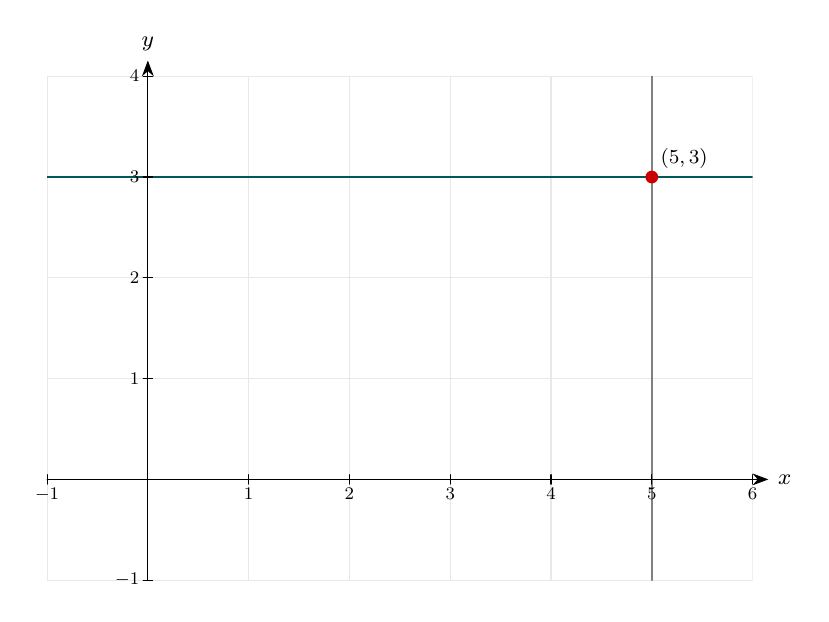
\begin{tikzpicture}[>={Stealth[length=2mm]},font=\footnotesize,line cap=round]
\begin{scope}
\clip (0,0) rectangle (8.96,6.4);
\draw[gray!18] (0,0) grid[xstep=1.28,ystep=1.28] (8.96,6.4);
\draw[gray,thick] (7.68,0) -- (7.68,6.4);
\draw[teal!70!black,thick] (0,5.12) -- (8.96,5.12);
\end{scope}
\draw[->] (0,1.28) -- (9.16,1.28) node[right]{$x$};
\draw[->] (1.28,0) -- (1.28,6.6) node[above]{$y$};
\draw (0,1.22) -- (0,1.34) node[below=2pt,scale=0.8]{$-1$};
\draw (2.56,1.22) -- (2.56,1.34) node[below=2pt,scale=0.8]{$1$};
\draw (3.84,1.22) -- (3.84,1.34) node[below=2pt,scale=0.8]{$2$};
\draw (5.12,1.22) -- (5.12,1.34) node[below=2pt,scale=0.8]{$3$};
\draw (6.4,1.22) -- (6.4,1.34) node[below=2pt,scale=0.8]{$4$};
\draw (7.68,1.22) -- (7.68,1.34) node[below=2pt,scale=0.8]{$5$};
\draw (8.96,1.22) -- (8.96,1.34) node[below=2pt,scale=0.8]{$6$};
\draw (1.22,0) -- (1.34,0) node[left=2pt,scale=0.8]{$-1$};
\draw (1.22,2.56) -- (1.34,2.56) node[left=2pt,scale=0.8]{$1$};
\draw (1.22,3.84) -- (1.34,3.84) node[left=2pt,scale=0.8]{$2$};
\draw (1.22,5.12) -- (1.34,5.12) node[left=2pt,scale=0.8]{$3$};
\draw (1.22,6.4) -- (1.34,6.4) node[left=2pt,scale=0.8]{$4$};
\fill[red!80!black] (7.68,5.12) circle (2.3pt);
\node[above right,scale=0.9] at (7.68,5.12) {$(5,3)$};
\end{tikzpicture}
}
\end{center}
\small The points and segments shown on the coordinate plane.\normalsize

\medskip\hrule

\section*{Line Segments 25\quad\small\texttt{(cg2-025)}}
\addcontentsline{toc}{section}{Line Segments 25 (cg2-025)}
\textit{Difficulty: Foundation \quad\textbar\quad Marks: 2}

\question{Find the midpoint of the line segment joining \( (2a, 3b) \) and \( (6a, -b) \).}

\textbf{Worked solution.}

\textit{Midpoint formula}
\[\begin{gathered}
M = \left(\frac{2a+6a}{2}, \frac{3b+(-b)}{2}\right) = (4a, b)
\end{gathered}\]
The midpoint formula works with algebraic expressions just as with numbers. Simplify: 8a/2 = 4a and 2b/2 = b.

\begin{answerbox}
\textbf{Final answer:}\quad \(\displaystyle (4a, b)\)
\end{answerbox}
\textbf{Diagram.}

\begin{center}
\resizebox{\ifdim\width>\linewidth \linewidth\else \width\fi}{!}{%
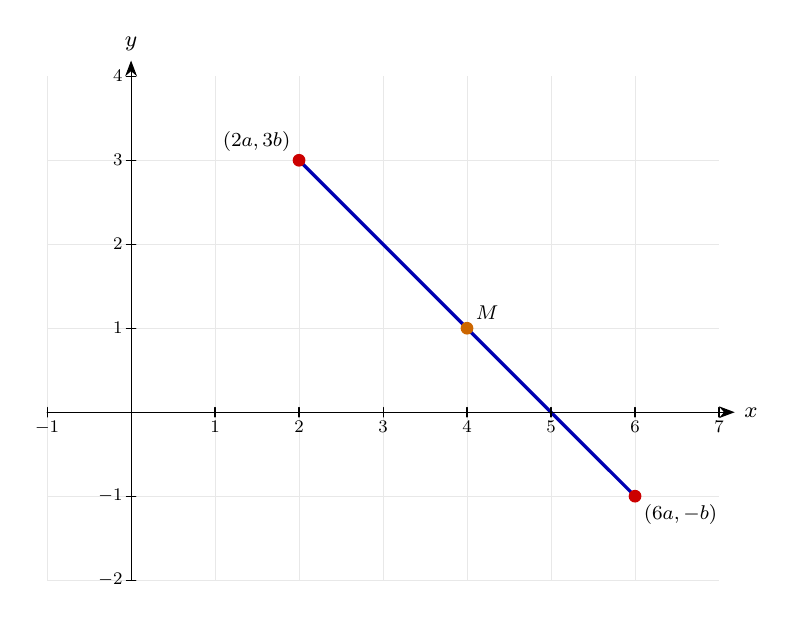
\begin{tikzpicture}[>={Stealth[length=2mm]},font=\footnotesize,line cap=round]
\begin{scope}
\clip (0,0) rectangle (8.533,6.4);
\draw[gray!18] (0,0) grid[xstep=1.067,ystep=1.067] (8.533,6.4);
\draw[blue!70!black,very thick] (3.2,5.333) -- (7.467,1.067);
\end{scope}
\draw[->] (0,2.133) -- (8.733,2.133) node[right]{$x$};
\draw[->] (1.067,0) -- (1.067,6.6) node[above]{$y$};
\draw (0,2.073) -- (0,2.193) node[below=2pt,scale=0.8]{$-1$};
\draw (2.133,2.073) -- (2.133,2.193) node[below=2pt,scale=0.8]{$1$};
\draw (3.2,2.073) -- (3.2,2.193) node[below=2pt,scale=0.8]{$2$};
\draw (4.267,2.073) -- (4.267,2.193) node[below=2pt,scale=0.8]{$3$};
\draw (5.333,2.073) -- (5.333,2.193) node[below=2pt,scale=0.8]{$4$};
\draw (6.4,2.073) -- (6.4,2.193) node[below=2pt,scale=0.8]{$5$};
\draw (7.467,2.073) -- (7.467,2.193) node[below=2pt,scale=0.8]{$6$};
\draw (8.533,2.073) -- (8.533,2.193) node[below=2pt,scale=0.8]{$7$};
\draw (1.007,0) -- (1.127,0) node[left=2pt,scale=0.8]{$-2$};
\draw (1.007,1.067) -- (1.127,1.067) node[left=2pt,scale=0.8]{$-1$};
\draw (1.007,3.2) -- (1.127,3.2) node[left=2pt,scale=0.8]{$1$};
\draw (1.007,4.267) -- (1.127,4.267) node[left=2pt,scale=0.8]{$2$};
\draw (1.007,5.333) -- (1.127,5.333) node[left=2pt,scale=0.8]{$3$};
\draw (1.007,6.4) -- (1.127,6.4) node[left=2pt,scale=0.8]{$4$};
\fill[red!80!black] (3.2,5.333) circle (2.3pt);
\node[above left,scale=0.9] at (3.2,5.333) {$(2a,3b)$};
\fill[red!80!black] (7.467,1.067) circle (2.3pt);
\node[below right,scale=0.9] at (7.467,1.067) {$(6a,-b)$};
\fill[orange!80!black] (5.333,3.2) circle (2.3pt);
\node[above right,scale=0.9] at (5.333,3.2) {$M$};
\end{tikzpicture}
}
\end{center}
\small The points and segments shown on the coordinate plane.\normalsize

\medskip\hrule

\section*{Line Segments 26\quad\small\texttt{(cg2-026)}}
\addcontentsline{toc}{section}{Line Segments 26 (cg2-026)}
\textit{Difficulty: Foundation \quad\textbar\quad Marks: 4}

\question{Show that \( A(0, 0) \), \( B(3, 4) \), \( C(8, 4) \), \( D(5, 0) \) form a parallelogram by showing the diagonals bisect each other.}

\textbf{Worked solution.}

\textit{Step 1: Identify the diagonals of quadrilateral ABCD.}
\[\begin{gathered}
\text{Diagonals: } AC \text{ and } BD
\end{gathered}\]
In a quadrilateral ABCD, the diagonals connect opposite vertices: A to C and B to D. A key property of a parallelogram is that its diagonals bisect each other --- they share the same midpoint.

\textit{Step 2: Find the midpoint of diagonal AC, where \( A(0,0) \) and \( C(8,4) \).}
\[\begin{gathered}
M_{AC} = \left(\frac{0+8}{2},\ \frac{0+4}{2}\right) = (4,\ 2)
\end{gathered}\]
Using the midpoint formula: add the x-coordinates and divide by 2, then add the y-coordinates and divide by 2.

\textit{Step 3: Find the midpoint of diagonal BD, where \( B(3,4) \) and \( D(5,0) \).}
\[\begin{gathered}
M_{BD} = \left(\frac{3+5}{2},\ \frac{4+0}{2}\right) = (4,\ 2)
\end{gathered}\]
Again applying the midpoint formula to the other diagonal.

\textit{Step 4: Compare the two midpoints.}
\[\begin{gathered}
M_{AC} = (4,\ 2) = M_{BD}
\end{gathered}\]
Both diagonals have the same midpoint (4, 2), which means they bisect each other. This is the defining property of a parallelogram, so ABCD is a parallelogram.

\begin{answerbox}
\textbf{Final answer:}\quad Diagonals AC and BD both have midpoint \(\displaystyle (4, 2)\), so they bisect each other, proving ABCD is a parallelogram.
\end{answerbox}
\textbf{Diagram.}

\begin{center}
\resizebox{\ifdim\width>\linewidth \linewidth\else \width\fi}{!}{%
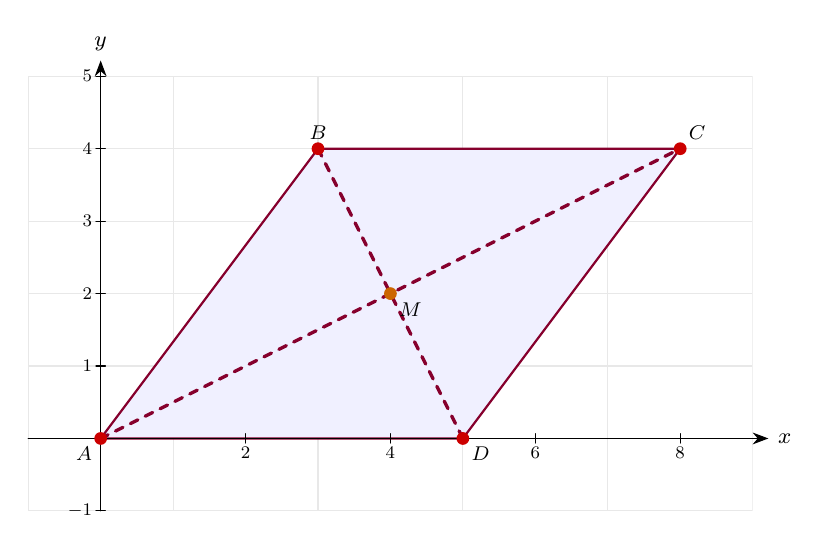
\begin{tikzpicture}[>={Stealth[length=2mm]},font=\footnotesize,line cap=round]
\begin{scope}
\clip (0,0) rectangle (9.2,5.52);
\draw[gray!18] (-0.92,0) grid[xstep=1.84,ystep=0.92] (9.2,5.52);
\fill[blue!6] (0.92,0.92) -- (3.68,4.6) -- (8.28,4.6) -- (5.52,0.92) -- cycle;
\draw[purple!70!black,thick] (0.92,0.92) -- (3.68,4.6) -- (8.28,4.6) -- (5.52,0.92) -- cycle;
\draw[dashed,purple!70!black,very thick] (0.92,0.92) -- (8.28,4.6);
\draw[dashed,purple!70!black,very thick] (3.68,4.6) -- (5.52,0.92);
\end{scope}
\draw[->] (0,0.92) -- (9.4,0.92) node[right]{$x$};
\draw[->] (0.92,0) -- (0.92,5.72) node[above]{$y$};
\draw (2.76,0.86) -- (2.76,0.98) node[below=2pt,scale=0.8]{$2$};
\draw (4.6,0.86) -- (4.6,0.98) node[below=2pt,scale=0.8]{$4$};
\draw (6.44,0.86) -- (6.44,0.98) node[below=2pt,scale=0.8]{$6$};
\draw (8.28,0.86) -- (8.28,0.98) node[below=2pt,scale=0.8]{$8$};
\draw (0.86,0) -- (0.98,0) node[left=2pt,scale=0.8]{$-1$};
\draw (0.86,1.84) -- (0.98,1.84) node[left=2pt,scale=0.8]{$1$};
\draw (0.86,2.76) -- (0.98,2.76) node[left=2pt,scale=0.8]{$2$};
\draw (0.86,3.68) -- (0.98,3.68) node[left=2pt,scale=0.8]{$3$};
\draw (0.86,4.6) -- (0.98,4.6) node[left=2pt,scale=0.8]{$4$};
\draw (0.86,5.52) -- (0.98,5.52) node[left=2pt,scale=0.8]{$5$};
\fill[red!80!black] (0.92,0.92) circle (2.3pt);
\node[below left,scale=0.9] at (0.92,0.92) {$A$};
\fill[red!80!black] (3.68,4.6) circle (2.3pt);
\node[above,scale=0.9] at (3.68,4.6) {$B$};
\fill[red!80!black] (8.28,4.6) circle (2.3pt);
\node[above right,scale=0.9] at (8.28,4.6) {$C$};
\fill[red!80!black] (5.52,0.92) circle (2.3pt);
\node[below right,scale=0.9] at (5.52,0.92) {$D$};
\fill[orange!80!black] (4.6,2.76) circle (2.3pt);
\node[below right,scale=0.9] at (4.6,2.76) {$M$};
\end{tikzpicture}
}
\end{center}
\small The points and segments shown on the coordinate plane.\normalsize

\medskip\hrule

\section*{Line Segments 27\quad\small\texttt{(cg2-027)}}
\addcontentsline{toc}{section}{Line Segments 27 (cg2-027)}
\textit{Difficulty: Foundation \quad\textbar\quad Marks: 3}

\question{Find the perimeter of the triangle with vertices \( A(0, 0) \), \( B(4, 0) \), \( C(0, 3) \).}

\textbf{Worked solution.}

\textit{Step 1: Find all side lengths}
\[\begin{gathered}
AB = 4, \quad AC = 3, \quad BC = \sqrt{16+9} = 5
\end{gathered}\]
AB and AC lie along the axes, so their lengths are just the coordinate differences. Only BC requires the full distance formula. This is a 3-4-5 right triangle.

\textit{Step 2: Sum}
\[\begin{gathered}
P = 4 + 3 + 5 = 12
\end{gathered}\]
The perimeter is the sum of all three side lengths.

\begin{answerbox}
\textbf{Final answer:}\quad \(\displaystyle 12\)
\end{answerbox}
\textbf{Diagram.}

\begin{center}
\resizebox{\ifdim\width>\linewidth \linewidth\else \width\fi}{!}{%
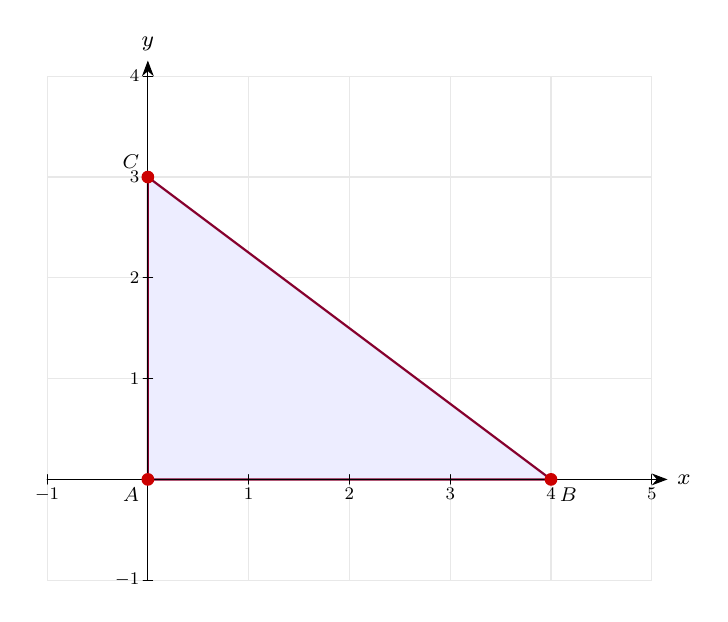
\begin{tikzpicture}[>={Stealth[length=2mm]},font=\footnotesize,line cap=round]
\begin{scope}
\clip (0,0) rectangle (7.68,6.4);
\draw[gray!18] (0,0) grid[xstep=1.28,ystep=1.28] (7.68,6.4);
\fill[blue!7] (1.28,1.28) -- (6.4,1.28) -- (1.28,5.12) -- cycle;
\draw[purple!70!black,thick] (1.28,1.28) -- (6.4,1.28) -- (1.28,5.12) -- cycle;
\end{scope}
\draw[->] (0,1.28) -- (7.88,1.28) node[right]{$x$};
\draw[->] (1.28,0) -- (1.28,6.6) node[above]{$y$};
\draw (0,1.22) -- (0,1.34) node[below=2pt,scale=0.8]{$-1$};
\draw (2.56,1.22) -- (2.56,1.34) node[below=2pt,scale=0.8]{$1$};
\draw (3.84,1.22) -- (3.84,1.34) node[below=2pt,scale=0.8]{$2$};
\draw (5.12,1.22) -- (5.12,1.34) node[below=2pt,scale=0.8]{$3$};
\draw (6.4,1.22) -- (6.4,1.34) node[below=2pt,scale=0.8]{$4$};
\draw (7.68,1.22) -- (7.68,1.34) node[below=2pt,scale=0.8]{$5$};
\draw (1.22,0) -- (1.34,0) node[left=2pt,scale=0.8]{$-1$};
\draw (1.22,2.56) -- (1.34,2.56) node[left=2pt,scale=0.8]{$1$};
\draw (1.22,3.84) -- (1.34,3.84) node[left=2pt,scale=0.8]{$2$};
\draw (1.22,5.12) -- (1.34,5.12) node[left=2pt,scale=0.8]{$3$};
\draw (1.22,6.4) -- (1.34,6.4) node[left=2pt,scale=0.8]{$4$};
\fill[red!80!black] (1.28,1.28) circle (2.3pt);
\node[below left,scale=0.9] at (1.28,1.28) {$A$};
\fill[red!80!black] (6.4,1.28) circle (2.3pt);
\node[below right,scale=0.9] at (6.4,1.28) {$B$};
\fill[red!80!black] (1.28,5.12) circle (2.3pt);
\node[above left,scale=0.9] at (1.28,5.12) {$C$};
\end{tikzpicture}
}
\end{center}
\small The points and segments shown on the coordinate plane.\normalsize

\medskip\hrule

\section*{Line Segments 28\quad\small\texttt{(cg2-028)}}
\addcontentsline{toc}{section}{Line Segments 28 (cg2-028)}
\textit{Difficulty: Foundation \quad\textbar\quad Marks: 3}

\question{The point \( P \) divides \( AB \) in the ratio \( 3:1 \), where \( A = (2, -1) \) and \( B = (10, 7) \). Find \( P \).}

\textbf{Worked solution.}

\textit{Step 1: Recall the section formula.}
\[\begin{gathered}
\text{If } P \text{ divides } AB \text{ in the ratio } m:n, \text{ then } P = \left(\frac{mx_2 + nx_1}{m+n},\ \frac{my_2 + ny_1}{m+n}\right)
\end{gathered}\]
The ratio 3:1 means P is three-quarters of the way from A to B, so P is much closer to B than to A.

\textit{Step 2: Identify the values: \( A(2, -1) \), \( B(10, 7) \), \( m = 3 \), \( n = 1 \).}
\[\begin{gathered}
x_1 = 2,\quad y_1 = -1,\quad x_2 = 10,\quad y_2 = 7
\end{gathered}\]
Here m = 3 (towards B) and n = 1 (towards A), and the total parts are m + n = 4.

\textit{Step 3: Calculate the x-coordinate of P.}
\[\begin{gathered}
x_P = \frac{3(10) + 1(2)}{3 + 1} = \frac{30 + 2}{4} = \frac{32}{4} = 8
\end{gathered}\]
Multiply x by m and x by n, then divide by the total number of parts.

\textit{Step 4: Calculate the y-coordinate of P.}
\[\begin{gathered}
y_P = \frac{3(7) + 1(-1)}{3 + 1} = \frac{21 - 1}{4} = \frac{20}{4} = 5
\end{gathered}\]
Same process for the y-coordinates.

\textit{Step 5: State the answer.}
\[\begin{gathered}
P = (8,\ 5)
\end{gathered}\]
We can verify: from A(2,-1) to P(8,5) the change is (+6, +6), and from P(8,5) to B(10,7) the change is (+2, +2). The ratio 6:2 = 3:1, confirming our answer.

\begin{answerbox}
\textbf{Final answer:}\quad \(\displaystyle P = (8,\ 5)\)
\end{answerbox}
\textbf{Diagram.}

\begin{center}
\resizebox{\ifdim\width>\linewidth \linewidth\else \width\fi}{!}{%
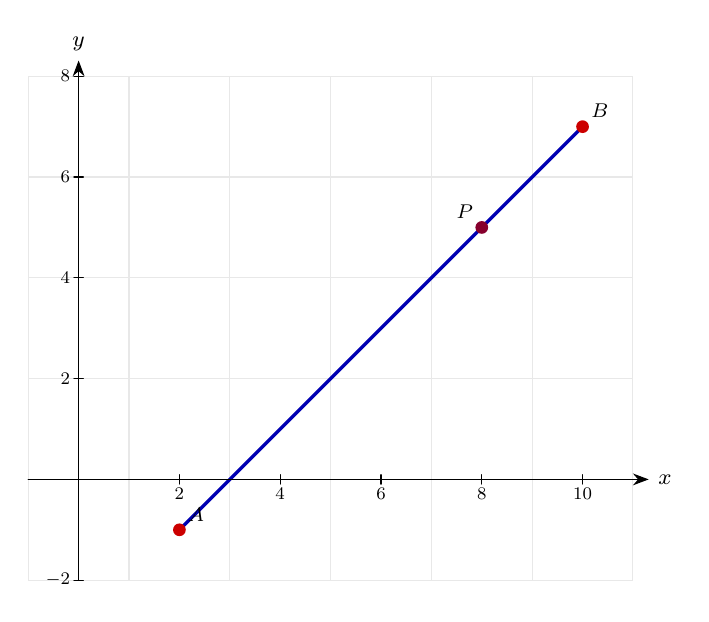
\begin{tikzpicture}[>={Stealth[length=2mm]},font=\footnotesize,line cap=round]
\begin{scope}
\clip (0,0) rectangle (7.68,6.4);
\draw[gray!18] (-0.64,0) grid[xstep=1.28,ystep=1.28] (7.68,6.4);
\draw[blue!70!black,very thick] (1.92,0.64) -- (7.04,5.76);
\end{scope}
\draw[->] (0,1.28) -- (7.88,1.28) node[right]{$x$};
\draw[->] (0.64,0) -- (0.64,6.6) node[above]{$y$};
\draw (1.92,1.22) -- (1.92,1.34) node[below=2pt,scale=0.8]{$2$};
\draw (3.2,1.22) -- (3.2,1.34) node[below=2pt,scale=0.8]{$4$};
\draw (4.48,1.22) -- (4.48,1.34) node[below=2pt,scale=0.8]{$6$};
\draw (5.76,1.22) -- (5.76,1.34) node[below=2pt,scale=0.8]{$8$};
\draw (7.04,1.22) -- (7.04,1.34) node[below=2pt,scale=0.8]{$10$};
\draw (0.58,0) -- (0.7,0) node[left=2pt,scale=0.8]{$-2$};
\draw (0.58,2.56) -- (0.7,2.56) node[left=2pt,scale=0.8]{$2$};
\draw (0.58,3.84) -- (0.7,3.84) node[left=2pt,scale=0.8]{$4$};
\draw (0.58,5.12) -- (0.7,5.12) node[left=2pt,scale=0.8]{$6$};
\draw (0.58,6.4) -- (0.7,6.4) node[left=2pt,scale=0.8]{$8$};
\fill[red!80!black] (1.92,0.64) circle (2.3pt);
\node[above right,scale=0.9] at (1.92,0.64) {$A$};
\fill[red!80!black] (7.04,5.76) circle (2.3pt);
\node[above right,scale=0.9] at (7.04,5.76) {$B$};
\fill[purple!70!black] (5.76,4.48) circle (2.3pt);
\node[above left,scale=0.9] at (5.76,4.48) {$P$};
\end{tikzpicture}
}
\end{center}
\small The points and segments shown on the coordinate plane.\normalsize

\medskip\hrule

\section*{Line Segments 29\quad\small\texttt{(cg2-029)}}
\addcontentsline{toc}{section}{Line Segments 29 (cg2-029)}
\textit{Difficulty: Foundation \quad\textbar\quad Marks: 2}

\question{Find the distance from the origin to the point \( (5, -12) \).}

\textbf{Worked solution.}

\textit{Step 1: Recall the distance formula.}
\[\begin{gathered}
d = \sqrt{(x_2 - x_1)^2 + (y_2 - y_1)^2}
\end{gathered}\]
The origin is the point (0, 0), so we use A(0, 0) and B(5, -12).

\textit{Step 2: Substitute the coordinates.}
\[\begin{gathered}
d = \sqrt{(5 - 0)^2 + (-12 - 0)^2} = \sqrt{5^2 + (-12)^2}
\end{gathered}\]
Subtract the x-coordinates and the y-coordinates separately, then square each difference.

\textit{Step 3: Evaluate the squares and add.}
\[\begin{gathered}
d = \sqrt{25 + 144} = \sqrt{169}
\end{gathered}\]
Note that (-12) = 144, not -144. Squaring always gives a positive result.

\textit{Step 4: Simplify the square root.}
\[\begin{gathered}
d = 13
\end{gathered}\]
169 = 13  13, so 169 = 13. This is a 5-12-13 Pythagorean triple.

\begin{answerbox}
\textbf{Final answer:}\quad \(\displaystyle 13\)
\end{answerbox}
\textbf{Diagram.}

\begin{center}
\resizebox{\ifdim\width>\linewidth \linewidth\else \width\fi}{!}{%
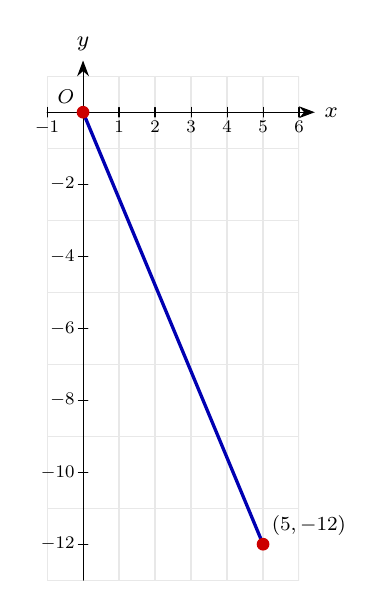
\begin{tikzpicture}[>={Stealth[length=2mm]},font=\footnotesize,line cap=round]
\begin{scope}
\clip (0,0) rectangle (3.2,6.4);
\draw[gray!18] (0,-0.457) grid[xstep=0.457,ystep=0.914] (3.2,6.4);
\draw[blue!70!black,very thick] (0.457,5.943) -- (2.743,0.457);
\end{scope}
\draw[->] (0,5.943) -- (3.4,5.943) node[right]{$x$};
\draw[->] (0.457,0) -- (0.457,6.6) node[above]{$y$};
\draw (0,5.883) -- (0,6.003) node[below=2pt,scale=0.8]{$-1$};
\draw (0.914,5.883) -- (0.914,6.003) node[below=2pt,scale=0.8]{$1$};
\draw (1.371,5.883) -- (1.371,6.003) node[below=2pt,scale=0.8]{$2$};
\draw (1.829,5.883) -- (1.829,6.003) node[below=2pt,scale=0.8]{$3$};
\draw (2.286,5.883) -- (2.286,6.003) node[below=2pt,scale=0.8]{$4$};
\draw (2.743,5.883) -- (2.743,6.003) node[below=2pt,scale=0.8]{$5$};
\draw (3.2,5.883) -- (3.2,6.003) node[below=2pt,scale=0.8]{$6$};
\draw (0.397,0.457) -- (0.517,0.457) node[left=2pt,scale=0.8]{$-12$};
\draw (0.397,1.371) -- (0.517,1.371) node[left=2pt,scale=0.8]{$-10$};
\draw (0.397,2.286) -- (0.517,2.286) node[left=2pt,scale=0.8]{$-8$};
\draw (0.397,3.2) -- (0.517,3.2) node[left=2pt,scale=0.8]{$-6$};
\draw (0.397,4.114) -- (0.517,4.114) node[left=2pt,scale=0.8]{$-4$};
\draw (0.397,5.029) -- (0.517,5.029) node[left=2pt,scale=0.8]{$-2$};
\fill[red!80!black] (0.457,5.943) circle (2.3pt);
\node[above left,scale=0.9] at (0.457,5.943) {$O$};
\fill[red!80!black] (2.743,0.457) circle (2.3pt);
\node[above right,scale=0.9] at (2.743,0.457) {$(5,-12)$};
\end{tikzpicture}
}
\end{center}
\small The points and segments shown on the coordinate plane.\normalsize

\medskip\hrule

\section*{Line Segments 30\quad\small\texttt{(cg2-030)}}
\addcontentsline{toc}{section}{Line Segments 30 (cg2-030)}
\textit{Difficulty: Foundation \quad\textbar\quad Marks: 4}

\question{The endpoints of a diameter of a circle are \( A(-2, 3) \) and \( B(6, -1) \). Find the centre and radius of the circle.}

\textbf{Worked solution.}

\textit{Step 1: Centre = midpoint}
\[\begin{gathered}
C = \left(\frac{-2+6}{2}, \frac{3+(-1)}{2}\right) = (2, 1)
\end{gathered}\]
The centre of a circle lies at the midpoint of any diameter.

\textit{Step 2: Radius = half diameter length}
\[\begin{gathered}
AB = \sqrt{64+16} = \sqrt{80} = 4\sqrt{5}, \quad r = 2\sqrt{5}
\end{gathered}\]
Find the full diameter length using the distance formula, then halve it. Simplify: sqrt(80) = sqrt(16 * 5) = 4*sqrt(5).

\begin{answerbox}
\textbf{Final answer:}\quad Centre \(\displaystyle (2, 1)\), radius \(\displaystyle 2\sqrt{5}\)
\end{answerbox}
\textbf{Diagram.}

\begin{center}
\resizebox{\ifdim\width>\linewidth \linewidth\else \width\fi}{!}{%
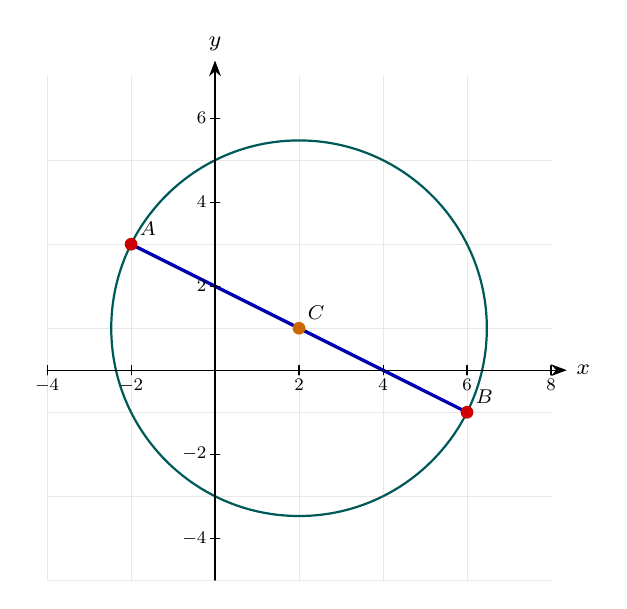
\begin{tikzpicture}[>={Stealth[length=2mm]},font=\footnotesize,line cap=round]
\begin{scope}
\clip (0,0) rectangle (6.4,6.4);
\draw[gray!18] (0,-0.533) grid[xstep=1.067,ystep=1.067] (6.4,6.4);
\draw[teal!70!black,thick] (3.2,3.2) circle (2.385);
\draw[blue!70!black,very thick] (1.067,4.267) -- (5.333,2.133);
\end{scope}
\draw[->] (0,2.667) -- (6.6,2.667) node[right]{$x$};
\draw[->] (2.133,0) -- (2.133,6.6) node[above]{$y$};
\draw (0,2.607) -- (0,2.727) node[below=2pt,scale=0.8]{$-4$};
\draw (1.067,2.607) -- (1.067,2.727) node[below=2pt,scale=0.8]{$-2$};
\draw (3.2,2.607) -- (3.2,2.727) node[below=2pt,scale=0.8]{$2$};
\draw (4.267,2.607) -- (4.267,2.727) node[below=2pt,scale=0.8]{$4$};
\draw (5.333,2.607) -- (5.333,2.727) node[below=2pt,scale=0.8]{$6$};
\draw (6.4,2.607) -- (6.4,2.727) node[below=2pt,scale=0.8]{$8$};
\draw (2.073,0.533) -- (2.193,0.533) node[left=2pt,scale=0.8]{$-4$};
\draw (2.073,1.6) -- (2.193,1.6) node[left=2pt,scale=0.8]{$-2$};
\draw (2.073,3.733) -- (2.193,3.733) node[left=2pt,scale=0.8]{$2$};
\draw (2.073,4.8) -- (2.193,4.8) node[left=2pt,scale=0.8]{$4$};
\draw (2.073,5.867) -- (2.193,5.867) node[left=2pt,scale=0.8]{$6$};
\fill[red!80!black] (1.067,4.267) circle (2.3pt);
\node[above right,scale=0.9] at (1.067,4.267) {$A$};
\fill[red!80!black] (5.333,2.133) circle (2.3pt);
\node[above right,scale=0.9] at (5.333,2.133) {$B$};
\fill[orange!80!black] (3.2,3.2) circle (2.3pt);
\node[above right,scale=0.9] at (3.2,3.2) {$C$};
\end{tikzpicture}
}
\end{center}
\small The points and segments shown on the coordinate plane.\normalsize

\medskip\hrule

\section*{Line Segments 31\quad\small\texttt{(cg2-031)}}
\addcontentsline{toc}{section}{Line Segments 31 (cg2-031)}
\textit{Difficulty: Foundation \quad\textbar\quad Marks: 4}

\question{Prove that the triangle with vertices \( (1, 1) \), \( (4, 5) \), \( (7, 1) \) is isosceles but not equilateral.}

\textbf{Worked solution.}

\textit{Step 1: Find all lengths}
\[\begin{gathered}
AB = \sqrt{9+16} = 5, \quad BC = \sqrt{9+16} = 5, \quad AC = 6
\end{gathered}\]
Use the distance formula for each pair. AC is horizontal (same y-coordinates), so its length is simply the difference in x-coordinates.

\textit{Step 2: Conclusion}
\[\begin{gathered}
AB = BC = 5 \neq AC = 6
\end{gathered}\]
Two sides equal so isosceles, but not all equal so not equilateral.

\begin{answerbox}
\textbf{Final answer:}\quad \(\displaystyle AB = BC = 5\), \(\displaystyle AC = 6\). Isosceles but not equilateral.
\end{answerbox}
\textbf{Diagram.}

\begin{center}
\resizebox{\ifdim\width>\linewidth \linewidth\else \width\fi}{!}{%
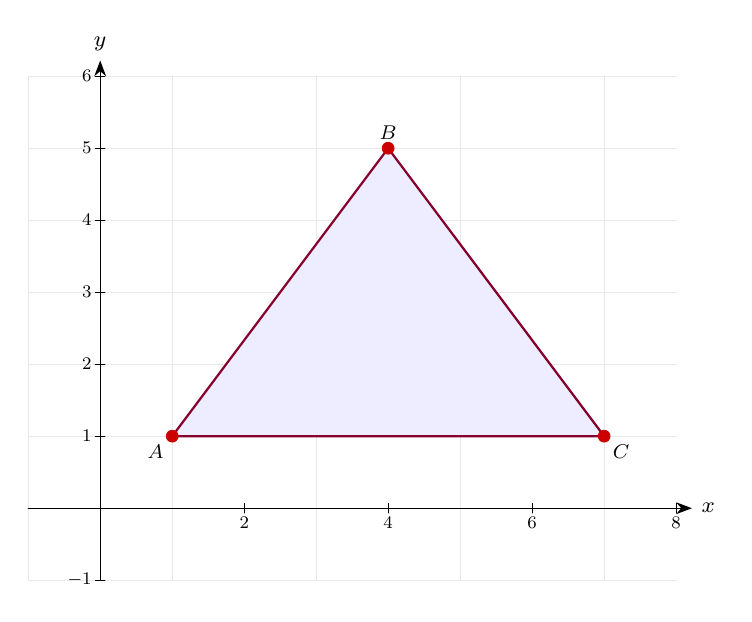
\begin{tikzpicture}[>={Stealth[length=2mm]},font=\footnotesize,line cap=round]
\begin{scope}
\clip (0,0) rectangle (8.229,6.4);
\draw[gray!18] (-0.914,0) grid[xstep=1.829,ystep=0.914] (8.229,6.4);
\fill[blue!7] (1.829,1.829) -- (4.571,5.486) -- (7.314,1.829) -- cycle;
\draw[purple!70!black,thick] (1.829,1.829) -- (4.571,5.486) -- (7.314,1.829) -- cycle;
\end{scope}
\draw[->] (0,0.914) -- (8.429,0.914) node[right]{$x$};
\draw[->] (0.914,0) -- (0.914,6.6) node[above]{$y$};
\draw (2.743,0.854) -- (2.743,0.974) node[below=2pt,scale=0.8]{$2$};
\draw (4.571,0.854) -- (4.571,0.974) node[below=2pt,scale=0.8]{$4$};
\draw (6.4,0.854) -- (6.4,0.974) node[below=2pt,scale=0.8]{$6$};
\draw (8.229,0.854) -- (8.229,0.974) node[below=2pt,scale=0.8]{$8$};
\draw (0.854,0) -- (0.974,0) node[left=2pt,scale=0.8]{$-1$};
\draw (0.854,1.829) -- (0.974,1.829) node[left=2pt,scale=0.8]{$1$};
\draw (0.854,2.743) -- (0.974,2.743) node[left=2pt,scale=0.8]{$2$};
\draw (0.854,3.657) -- (0.974,3.657) node[left=2pt,scale=0.8]{$3$};
\draw (0.854,4.571) -- (0.974,4.571) node[left=2pt,scale=0.8]{$4$};
\draw (0.854,5.486) -- (0.974,5.486) node[left=2pt,scale=0.8]{$5$};
\draw (0.854,6.4) -- (0.974,6.4) node[left=2pt,scale=0.8]{$6$};
\fill[red!80!black] (1.829,1.829) circle (2.3pt);
\node[below left,scale=0.9] at (1.829,1.829) {$A$};
\fill[red!80!black] (4.571,5.486) circle (2.3pt);
\node[above,scale=0.9] at (4.571,5.486) {$B$};
\fill[red!80!black] (7.314,1.829) circle (2.3pt);
\node[below right,scale=0.9] at (7.314,1.829) {$C$};
\end{tikzpicture}
}
\end{center}
\small The points and segments shown on the coordinate plane.\normalsize

\medskip\hrule

\section*{Line Segments 32\quad\small\texttt{(cg2-032)}}
\addcontentsline{toc}{section}{Line Segments 32 (cg2-032)}
\textit{Difficulty: Foundation \quad\textbar\quad Marks: 4}

\question{The midpoint of \( AB \) is \( M(4, -2) \) and \( A = (1, 3) \). Find \( B \) and the length \( AB \).}

\textbf{Worked solution.}

\textit{Step 1: Find B}
\[\begin{gathered}
B = (2(4)-1, 2(-2)-3) = (7, -7)
\end{gathered}\]
Rearranging the midpoint formula: x\_B = 2*x\_M - x\_A and y\_B = 2*y\_M - y\_A.

\textit{Step 2: Length}
\[\begin{gathered}
AB = \sqrt{36+100} = \sqrt{136} = 2\sqrt{34}
\end{gathered}\]
Apply the distance formula between A(1, 3) and B(7, -7). Simplify: sqrt(136) = sqrt(4 * 34) = 2*sqrt(34).

\begin{answerbox}
\textbf{Final answer:}\quad \(\displaystyle B = (7, -7), AB = 2\sqrt{34}\)
\end{answerbox}
\textbf{Diagram.}

\begin{center}
\resizebox{\ifdim\width>\linewidth \linewidth\else \width\fi}{!}{%
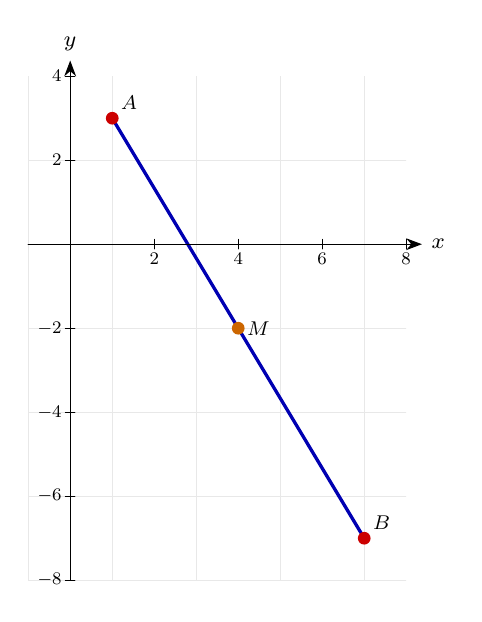
\begin{tikzpicture}[>={Stealth[length=2mm]},font=\footnotesize,line cap=round]
\begin{scope}
\clip (0,0) rectangle (4.8,6.4);
\draw[gray!18] (-0.533,0) grid[xstep=1.067,ystep=1.067] (4.8,6.4);
\draw[blue!70!black,very thick] (1.067,5.867) -- (4.267,0.533);
\end{scope}
\draw[->] (0,4.267) -- (5,4.267) node[right]{$x$};
\draw[->] (0.533,0) -- (0.533,6.6) node[above]{$y$};
\draw (1.6,4.207) -- (1.6,4.327) node[below=2pt,scale=0.8]{$2$};
\draw (2.667,4.207) -- (2.667,4.327) node[below=2pt,scale=0.8]{$4$};
\draw (3.733,4.207) -- (3.733,4.327) node[below=2pt,scale=0.8]{$6$};
\draw (4.8,4.207) -- (4.8,4.327) node[below=2pt,scale=0.8]{$8$};
\draw (0.473,0) -- (0.593,0) node[left=2pt,scale=0.8]{$-8$};
\draw (0.473,1.067) -- (0.593,1.067) node[left=2pt,scale=0.8]{$-6$};
\draw (0.473,2.133) -- (0.593,2.133) node[left=2pt,scale=0.8]{$-4$};
\draw (0.473,3.2) -- (0.593,3.2) node[left=2pt,scale=0.8]{$-2$};
\draw (0.473,5.333) -- (0.593,5.333) node[left=2pt,scale=0.8]{$2$};
\draw (0.473,6.4) -- (0.593,6.4) node[left=2pt,scale=0.8]{$4$};
\fill[red!80!black] (1.067,5.867) circle (2.3pt);
\node[above right,scale=0.9] at (1.067,5.867) {$A$};
\fill[red!80!black] (4.267,0.533) circle (2.3pt);
\node[above right,scale=0.9] at (4.267,0.533) {$B$};
\fill[orange!80!black] (2.667,3.2) circle (2.3pt);
\node[right,scale=0.9] at (2.667,3.2) {$M$};
\end{tikzpicture}
}
\end{center}
\small The points and segments shown on the coordinate plane.\normalsize

\medskip\hrule

\section*{Line Segments 33\quad\small\texttt{(cg2-033)}}
\addcontentsline{toc}{section}{Line Segments 33 (cg2-033)}
\textit{Difficulty: Foundation \quad\textbar\quad Marks: 2}

\question{Find the point that divides \( A(0, 0) \) to \( B(12, 8) \) in the ratio \( 2:1 \).}

\textbf{Worked solution.}

\textit{Section formula}
\[\begin{gathered}
P = \left(\frac{2(12)}{3}, \frac{2(8)}{3}\right) = (8, \tfrac{16}{3})
\end{gathered}\]
The ratio 2:1 means P is two-thirds of the way from A to B. Since A is the origin, each coordinate of P is simply 2/3 of the corresponding coordinate of B.

\begin{answerbox}
\textbf{Final answer:}\quad \(\displaystyle \left(8, \frac{16}{3}\right)\)
\end{answerbox}
\textbf{Diagram.}

\begin{center}
\resizebox{\ifdim\width>\linewidth \linewidth\else \width\fi}{!}{%
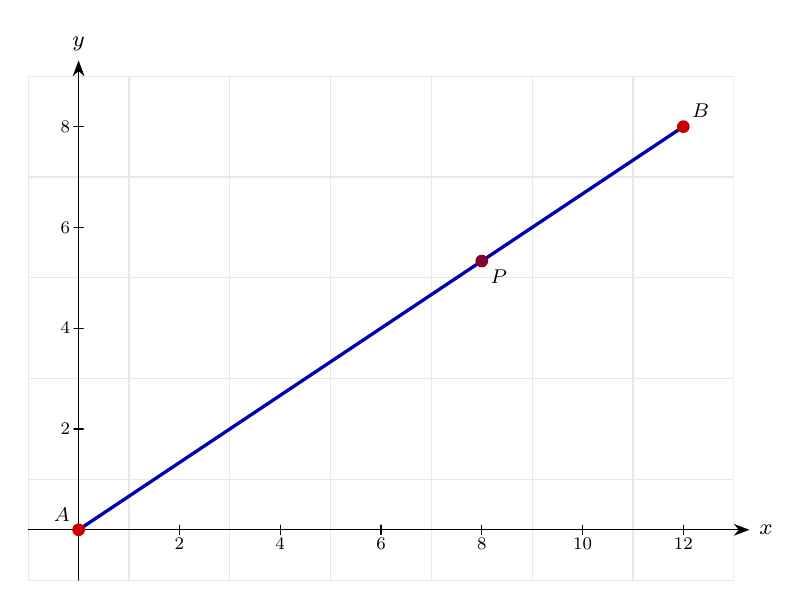
\begin{tikzpicture}[>={Stealth[length=2mm]},font=\footnotesize,line cap=round]
\begin{scope}
\clip (0,0) rectangle (8.96,6.4);
\draw[gray!18] (-0.64,-0.64) grid[xstep=1.28,ystep=1.28] (8.96,6.4);
\draw[blue!70!black,very thick] (0.64,0.64) -- (8.32,5.76);
\end{scope}
\draw[->] (0,0.64) -- (9.16,0.64) node[right]{$x$};
\draw[->] (0.64,0) -- (0.64,6.6) node[above]{$y$};
\draw (1.92,0.58) -- (1.92,0.7) node[below=2pt,scale=0.8]{$2$};
\draw (3.2,0.58) -- (3.2,0.7) node[below=2pt,scale=0.8]{$4$};
\draw (4.48,0.58) -- (4.48,0.7) node[below=2pt,scale=0.8]{$6$};
\draw (5.76,0.58) -- (5.76,0.7) node[below=2pt,scale=0.8]{$8$};
\draw (7.04,0.58) -- (7.04,0.7) node[below=2pt,scale=0.8]{$10$};
\draw (8.32,0.58) -- (8.32,0.7) node[below=2pt,scale=0.8]{$12$};
\draw (0.58,1.92) -- (0.7,1.92) node[left=2pt,scale=0.8]{$2$};
\draw (0.58,3.2) -- (0.7,3.2) node[left=2pt,scale=0.8]{$4$};
\draw (0.58,4.48) -- (0.7,4.48) node[left=2pt,scale=0.8]{$6$};
\draw (0.58,5.76) -- (0.7,5.76) node[left=2pt,scale=0.8]{$8$};
\fill[red!80!black] (0.64,0.64) circle (2.3pt);
\node[above left,scale=0.9] at (0.64,0.64) {$A$};
\fill[red!80!black] (8.32,5.76) circle (2.3pt);
\node[above right,scale=0.9] at (8.32,5.76) {$B$};
\fill[purple!70!black] (5.76,4.053) circle (2.3pt);
\node[below right,scale=0.9] at (5.76,4.053) {$P$};
\end{tikzpicture}
}
\end{center}
\small The points and segments shown on the coordinate plane.\normalsize

\medskip\hrule

\section*{Line Segments 34\quad\small\texttt{(cg2-034)}}
\addcontentsline{toc}{section}{Line Segments 34 (cg2-034)}
\textit{Difficulty: Foundation \quad\textbar\quad Marks: 4}

\question{Show that the points \( A(2, 3) \), \( B(5, 7) \), \( C(9, 4) \) form a right-angled triangle at \( B \).}

\textbf{Worked solution.}

\textit{Step 1: Find lengths squared}
\[\begin{gathered}
AB^2 = 3^2+4^2 = 25, \quad BC^2 = 4^2+(-3)^2 = 25, \quad AC^2 = 7^2+1^2 = 50
\end{gathered}\]
Working with squared lengths avoids square roots and lets us check Pythagoras directly.

\textit{Step 2: Check Pythagoras}
\[\begin{gathered}
AB^2 + BC^2 = 25 + 25 = 50 = AC^2
\end{gathered}\]
Since the two shorter sides meet at B and their squares add to the square of AC, the right angle is at B.

\textit{Step 3: Check perpendicular gradients}
\[\begin{gathered}
m_{AB} = \frac{4}{3}, \quad m_{BC} = \frac{-3}{4}, \quad m_{AB} \times m_{BC} = -1
\end{gathered}\]
The gradients are negative reciprocals, so AB is perpendicular to BC. This confirms the right angle at B.

\begin{answerbox}
\textbf{Final answer:}\quad Right-angled at \(\displaystyle B\), with \(\displaystyle AB = BC = 5\) and \(\displaystyle AC = 5\sqrt{2}\).
\end{answerbox}
\textbf{Diagram.}

\begin{center}
\resizebox{\ifdim\width>\linewidth \linewidth\else \width\fi}{!}{%
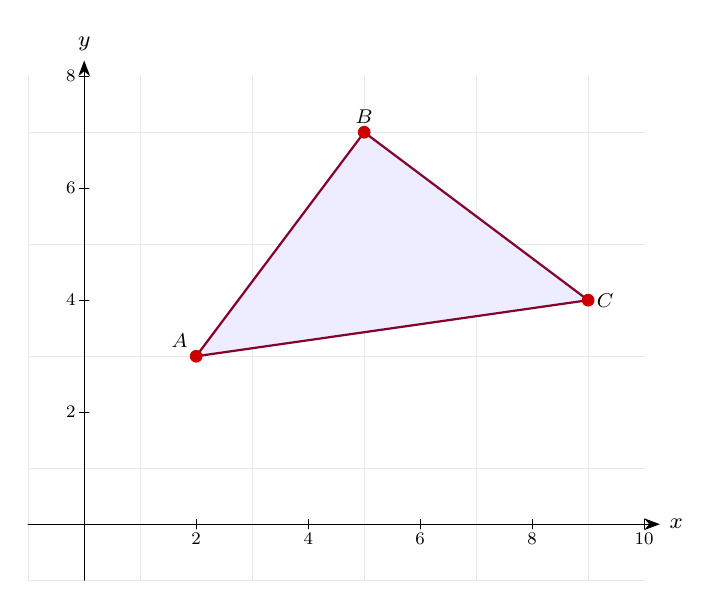
\begin{tikzpicture}[>={Stealth[length=2mm]},font=\footnotesize,line cap=round]
\begin{scope}
\clip (0,0) rectangle (7.822,6.4);
\draw[gray!18] (-0.711,-0.711) grid[xstep=1.422,ystep=1.422] (7.822,6.4);
\fill[blue!7] (2.133,2.844) -- (4.267,5.689) -- (7.111,3.556) -- cycle;
\draw[purple!70!black,thick] (2.133,2.844) -- (4.267,5.689) -- (7.111,3.556) -- cycle;
\end{scope}
\draw[->] (0,0.711) -- (8.022,0.711) node[right]{$x$};
\draw[->] (0.711,0) -- (0.711,6.6) node[above]{$y$};
\draw (2.133,0.651) -- (2.133,0.771) node[below=2pt,scale=0.8]{$2$};
\draw (3.556,0.651) -- (3.556,0.771) node[below=2pt,scale=0.8]{$4$};
\draw (4.978,0.651) -- (4.978,0.771) node[below=2pt,scale=0.8]{$6$};
\draw (6.4,0.651) -- (6.4,0.771) node[below=2pt,scale=0.8]{$8$};
\draw (7.822,0.651) -- (7.822,0.771) node[below=2pt,scale=0.8]{$10$};
\draw (0.651,2.133) -- (0.771,2.133) node[left=2pt,scale=0.8]{$2$};
\draw (0.651,3.556) -- (0.771,3.556) node[left=2pt,scale=0.8]{$4$};
\draw (0.651,4.978) -- (0.771,4.978) node[left=2pt,scale=0.8]{$6$};
\draw (0.651,6.4) -- (0.771,6.4) node[left=2pt,scale=0.8]{$8$};
\fill[red!80!black] (2.133,2.844) circle (2.3pt);
\node[above left,scale=0.9] at (2.133,2.844) {$A$};
\fill[red!80!black] (4.267,5.689) circle (2.3pt);
\node[above,scale=0.9] at (4.267,5.689) {$B$};
\fill[red!80!black] (7.111,3.556) circle (2.3pt);
\node[right,scale=0.9] at (7.111,3.556) {$C$};
\end{tikzpicture}
}
\end{center}
\small The points and segments shown on the coordinate plane.\normalsize

\medskip\hrule

\section*{Line Segments 35\quad\small\texttt{(cg2-035)}}
\addcontentsline{toc}{section}{Line Segments 35 (cg2-035)}
\textit{Difficulty: Foundation \quad\textbar\quad Marks: 2}

\question{Find the distance between \( A(1, -2) \) and \( B(-3, 1) \). Leave your answer as a surd.}

\textbf{Worked solution.}

\textit{Distance formula}
\[\begin{gathered}
AB = \sqrt{(-3-1)^2 + (1-(-2))^2} = \sqrt{16+9} = 5
\end{gathered}\]
Note that (-3-1)\textasciicircum 2 = 16 and (1-(-2))\textasciicircum 2 = 9. The answer is a whole number (3-4-5 triple), so no surd is needed despite the question asking for one.

\begin{answerbox}
\textbf{Final answer:}\quad \(\displaystyle 5\)
\end{answerbox}
\textbf{Diagram.}

\begin{center}
\resizebox{\ifdim\width>\linewidth \linewidth\else \width\fi}{!}{%
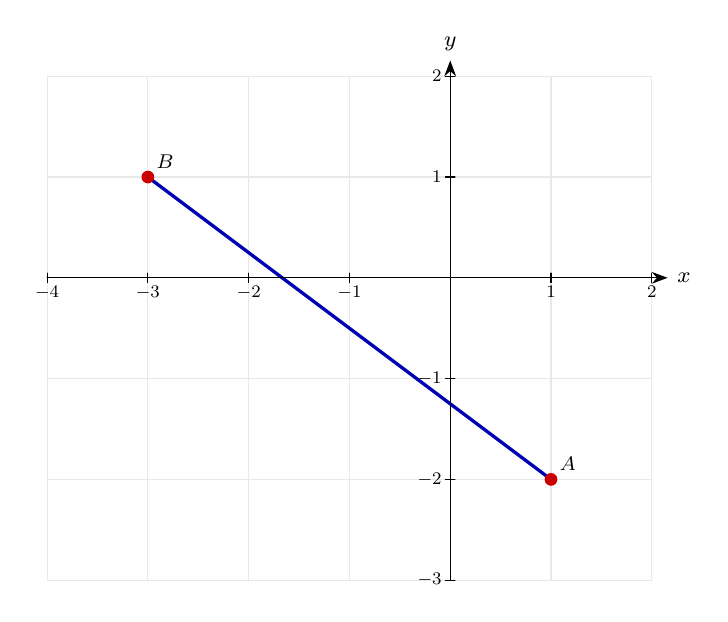
\begin{tikzpicture}[>={Stealth[length=2mm]},font=\footnotesize,line cap=round]
\begin{scope}
\clip (0,0) rectangle (7.68,6.4);
\draw[gray!18] (0,0) grid[xstep=1.28,ystep=1.28] (7.68,6.4);
\draw[blue!70!black,very thick] (6.4,1.28) -- (1.28,5.12);
\end{scope}
\draw[->] (0,3.84) -- (7.88,3.84) node[right]{$x$};
\draw[->] (5.12,0) -- (5.12,6.6) node[above]{$y$};
\draw (0,3.78) -- (0,3.9) node[below=2pt,scale=0.8]{$-4$};
\draw (1.28,3.78) -- (1.28,3.9) node[below=2pt,scale=0.8]{$-3$};
\draw (2.56,3.78) -- (2.56,3.9) node[below=2pt,scale=0.8]{$-2$};
\draw (3.84,3.78) -- (3.84,3.9) node[below=2pt,scale=0.8]{$-1$};
\draw (6.4,3.78) -- (6.4,3.9) node[below=2pt,scale=0.8]{$1$};
\draw (7.68,3.78) -- (7.68,3.9) node[below=2pt,scale=0.8]{$2$};
\draw (5.06,0) -- (5.18,0) node[left=2pt,scale=0.8]{$-3$};
\draw (5.06,1.28) -- (5.18,1.28) node[left=2pt,scale=0.8]{$-2$};
\draw (5.06,2.56) -- (5.18,2.56) node[left=2pt,scale=0.8]{$-1$};
\draw (5.06,5.12) -- (5.18,5.12) node[left=2pt,scale=0.8]{$1$};
\draw (5.06,6.4) -- (5.18,6.4) node[left=2pt,scale=0.8]{$2$};
\fill[red!80!black] (6.4,1.28) circle (2.3pt);
\node[above right,scale=0.9] at (6.4,1.28) {$A$};
\fill[red!80!black] (1.28,5.12) circle (2.3pt);
\node[above right,scale=0.9] at (1.28,5.12) {$B$};
\end{tikzpicture}
}
\end{center}
\small The points and segments shown on the coordinate plane.\normalsize

\medskip\hrule

\section*{Line Segments 36\quad\small\texttt{(cg2-036)}}
\addcontentsline{toc}{section}{Line Segments 36 (cg2-036)}
\textit{Difficulty: Foundation \quad\textbar\quad Marks: 5}

\question{M is the midpoint of \( AB \) where \( A = (-4, 6) \) and \( B = (2, -8) \). Find the gradient of \( AB \) and the equation of the perpendicular bisector.}

\textbf{Worked solution.}

\textit{Step 1: Midpoint}
\[\begin{gathered}
M = (-1, -1)
\end{gathered}\]
Using the midpoint formula: average the x-coordinates and average the y-coordinates separately.

\textit{Step 2: Gradient of AB}
\[\begin{gathered}
m = \frac{-8-6}{2-(-4)} = \frac{-14}{6} = -\frac{7}{3}
\end{gathered}\]
Gradient = rise over run. Be careful with double negatives: \(2 - (-4) = 6\), not \(2\).

\textit{Step 3: Perpendicular bisector}
\[\begin{gathered}
m_{\perp} = \frac{3}{7}; \quad y + 1 = \frac{3}{7}(x + 1) \implies 7y = 3x - 4
\end{gathered}\]
The perpendicular gradient is the negative reciprocal. Then use \(y - y_1 = m(x - x_1)\) with the midpoint as \((x_1, y_1)\).

\begin{answerbox}
\textbf{Final answer:}\quad Gradient of \(\displaystyle AB\): \(\displaystyle -\frac{7}{3}\); perpendicular bisector: \(\displaystyle 3x - 7y - 4 = 0\)
\end{answerbox}
\textbf{Diagram.}

\begin{center}
\resizebox{\ifdim\width>\linewidth \linewidth\else \width\fi}{!}{%
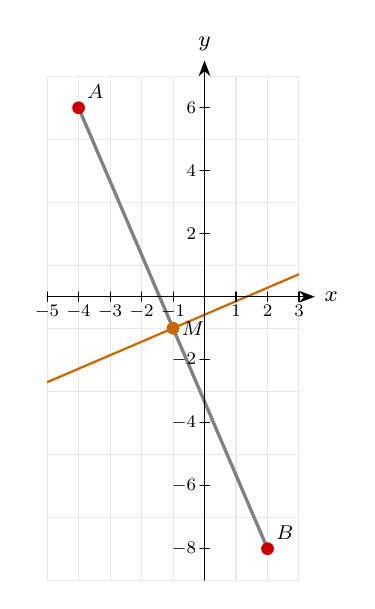
\begin{tikzpicture}[>={Stealth[length=2mm]},font=\footnotesize,line cap=round]
\begin{scope}
\clip (0,0) rectangle (3.2,6.4);
\draw[gray!18] (0,-0.4) grid[xstep=0.4,ystep=0.8] (3.2,6.4);
\draw[orange!80!black,thick] (0,2.514) -- (3.2,3.886);
\draw[gray,very thick] (0.4,6) -- (2.8,0.4);
\end{scope}
\draw[->] (0,3.6) -- (3.4,3.6) node[right]{$x$};
\draw[->] (2,0) -- (2,6.6) node[above]{$y$};
\draw (0,3.54) -- (0,3.66) node[below=2pt,scale=0.8]{$-5$};
\draw (0.4,3.54) -- (0.4,3.66) node[below=2pt,scale=0.8]{$-4$};
\draw (0.8,3.54) -- (0.8,3.66) node[below=2pt,scale=0.8]{$-3$};
\draw (1.2,3.54) -- (1.2,3.66) node[below=2pt,scale=0.8]{$-2$};
\draw (1.6,3.54) -- (1.6,3.66) node[below=2pt,scale=0.8]{$-1$};
\draw (2.4,3.54) -- (2.4,3.66) node[below=2pt,scale=0.8]{$1$};
\draw (2.8,3.54) -- (2.8,3.66) node[below=2pt,scale=0.8]{$2$};
\draw (3.2,3.54) -- (3.2,3.66) node[below=2pt,scale=0.8]{$3$};
\draw (1.94,0.4) -- (2.06,0.4) node[left=2pt,scale=0.8]{$-8$};
\draw (1.94,1.2) -- (2.06,1.2) node[left=2pt,scale=0.8]{$-6$};
\draw (1.94,2) -- (2.06,2) node[left=2pt,scale=0.8]{$-4$};
\draw (1.94,2.8) -- (2.06,2.8) node[left=2pt,scale=0.8]{$-2$};
\draw (1.94,4.4) -- (2.06,4.4) node[left=2pt,scale=0.8]{$2$};
\draw (1.94,5.2) -- (2.06,5.2) node[left=2pt,scale=0.8]{$4$};
\draw (1.94,6) -- (2.06,6) node[left=2pt,scale=0.8]{$6$};
\fill[red!80!black] (0.4,6) circle (2.3pt);
\node[above right,scale=0.9] at (0.4,6) {$A$};
\fill[red!80!black] (2.8,0.4) circle (2.3pt);
\node[above right,scale=0.9] at (2.8,0.4) {$B$};
\fill[orange!80!black] (1.6,3.2) circle (2.3pt);
\node[right,scale=0.9] at (1.6,3.2) {$M$};
\end{tikzpicture}
}
\end{center}
\small The points and segments shown on the coordinate plane.\normalsize

\medskip\hrule

\section*{Line Segments 37\quad\small\texttt{(cg2-037)}}
\addcontentsline{toc}{section}{Line Segments 37 (cg2-037)}
\textit{Difficulty: Foundation \quad\textbar\quad Marks: 5}

\question{The three vertices of a triangle are \( A(0, 0) \), \( B(8, 0) \) and \( C(4, 6) \). Find the lengths of the three medians.}

\textbf{Worked solution.}

\textit{Step 1: Midpoints of sides}
\[\begin{gathered}
M_{BC} = (6, 3), \quad M_{AC} = (2, 3), \quad M_{AB} = (4, 0)
\end{gathered}\]
A median connects a vertex to the midpoint of the opposite side, so first find all three midpoints.

\textit{Step 2: Median from A}
\[\begin{gathered}
AM_{BC} = \sqrt{36+9} = \sqrt{45} = 3\sqrt{5}
\end{gathered}\]
Distance from A(0,0) to M\_\{BC\}(6,3). Simplify: \(\sqrt{45} = \sqrt{9 \times 5} = 3\sqrt{5}\).

\textit{Step 3: Median from B}
\[\begin{gathered}
BM_{AC} = \sqrt{36+9} = 3\sqrt{5}
\end{gathered}\]
Distance from B(8,0) to M\_\{AC\}(2,3). Two medians have equal length, reflecting the symmetry of the triangle.

\textit{Step 4: Median from C}
\[\begin{gathered}
CM_{AB} = \sqrt{0+36} = 6
\end{gathered}\]
Distance from C(4,6) to M\_\{AB\}(4,0). Since they share the same x-coordinate, the distance is simply the difference in y-coordinates.

\begin{answerbox}
\textbf{Final answer:}\quad \(\displaystyle 3\sqrt{5}, 3\sqrt{5}, 6\)
\end{answerbox}
\textbf{Diagram.}

\begin{center}
\resizebox{\ifdim\width>\linewidth \linewidth\else \width\fi}{!}{%
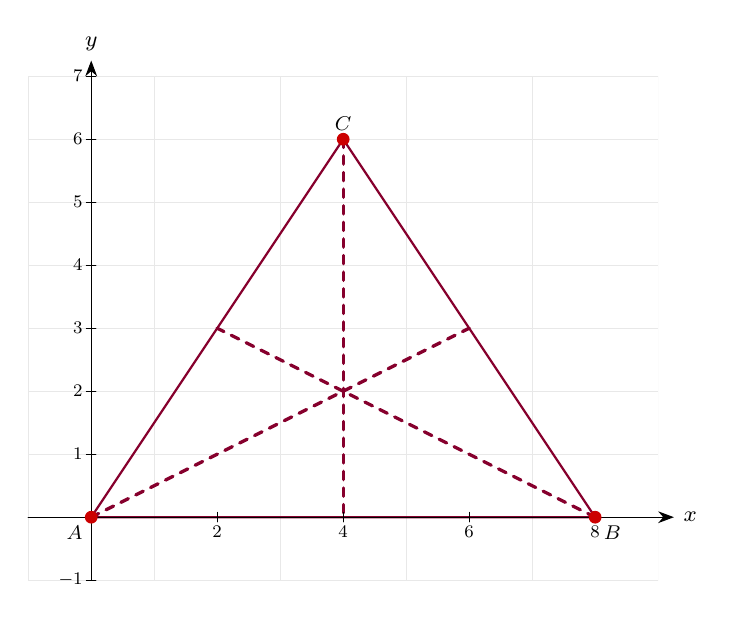
\begin{tikzpicture}[>={Stealth[length=2mm]},font=\footnotesize,line cap=round]
\begin{scope}
\clip (0,0) rectangle (8,6.4);
\draw[gray!18] (-0.8,0) grid[xstep=1.6,ystep=0.8] (8,6.4);
\draw[purple!70!black,thick] (0.8,0.8) -- (7.2,0.8) -- (4,5.6) -- cycle;
\draw[dashed,purple!70!black,very thick] (0.8,0.8) -- (5.6,3.2);
\draw[dashed,purple!70!black,very thick] (7.2,0.8) -- (2.4,3.2);
\draw[dashed,purple!70!black,very thick] (4,5.6) -- (4,0.8);
\end{scope}
\draw[->] (0,0.8) -- (8.2,0.8) node[right]{$x$};
\draw[->] (0.8,0) -- (0.8,6.6) node[above]{$y$};
\draw (2.4,0.74) -- (2.4,0.86) node[below=2pt,scale=0.8]{$2$};
\draw (4,0.74) -- (4,0.86) node[below=2pt,scale=0.8]{$4$};
\draw (5.6,0.74) -- (5.6,0.86) node[below=2pt,scale=0.8]{$6$};
\draw (7.2,0.74) -- (7.2,0.86) node[below=2pt,scale=0.8]{$8$};
\draw (0.74,0) -- (0.86,0) node[left=2pt,scale=0.8]{$-1$};
\draw (0.74,1.6) -- (0.86,1.6) node[left=2pt,scale=0.8]{$1$};
\draw (0.74,2.4) -- (0.86,2.4) node[left=2pt,scale=0.8]{$2$};
\draw (0.74,3.2) -- (0.86,3.2) node[left=2pt,scale=0.8]{$3$};
\draw (0.74,4) -- (0.86,4) node[left=2pt,scale=0.8]{$4$};
\draw (0.74,4.8) -- (0.86,4.8) node[left=2pt,scale=0.8]{$5$};
\draw (0.74,5.6) -- (0.86,5.6) node[left=2pt,scale=0.8]{$6$};
\draw (0.74,6.4) -- (0.86,6.4) node[left=2pt,scale=0.8]{$7$};
\fill[red!80!black] (0.8,0.8) circle (2.3pt);
\node[below left,scale=0.9] at (0.8,0.8) {$A$};
\fill[red!80!black] (7.2,0.8) circle (2.3pt);
\node[below right,scale=0.9] at (7.2,0.8) {$B$};
\fill[red!80!black] (4,5.6) circle (2.3pt);
\node[above,scale=0.9] at (4,5.6) {$C$};
\end{tikzpicture}
}
\end{center}
\small The points and segments shown on the coordinate plane.\normalsize

\medskip\hrule

\section*{Line Segments 38\quad\small\texttt{(cg2-038)}}
\addcontentsline{toc}{section}{Line Segments 38 (cg2-038)}
\textit{Difficulty: Foundation \quad\textbar\quad Marks: 3}

\question{A line segment has endpoints \( (1, 5) \) and \( (9, 1) \). Find the point that is \( \frac{3}{4} \) of the way from the first to the second endpoint.}

\textbf{Worked solution.}

\textit{Use ratio 3:1}
\[\begin{gathered}
P = \left(1 + \frac{3}{4}(9-1), 5 + \frac{3}{4}(1-5)\right) = (7, 2)
\end{gathered}\]
Being \(\frac{3}{4}\) of the way along is equivalent to dividing the segment in the ratio 3:1. Add \(\frac{3}{4}\) of the change in each coordinate to the starting point.

\begin{answerbox}
\textbf{Final answer:}\quad \(\displaystyle (7, 2)\)
\end{answerbox}
\textbf{Diagram.}

\begin{center}
\resizebox{\ifdim\width>\linewidth \linewidth\else \width\fi}{!}{%
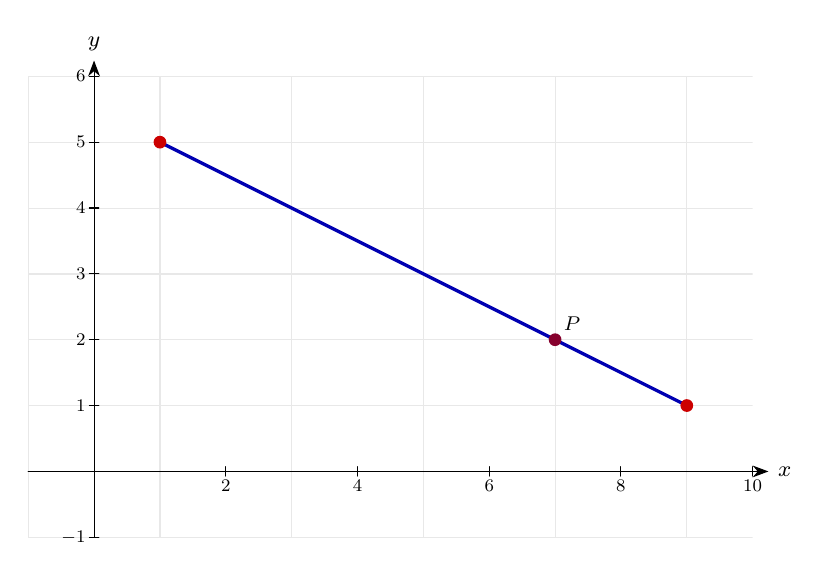
\begin{tikzpicture}[>={Stealth[length=2mm]},font=\footnotesize,line cap=round]
\begin{scope}
\clip (0,0) rectangle (9.2,5.855);
\draw[gray!18] (-0.836,0) grid[xstep=1.673,ystep=0.836] (9.2,5.855);
\draw[blue!70!black,very thick] (1.673,5.018) -- (8.364,1.673);
\end{scope}
\draw[->] (0,0.836) -- (9.4,0.836) node[right]{$x$};
\draw[->] (0.836,0) -- (0.836,6.055) node[above]{$y$};
\draw (2.509,0.776) -- (2.509,0.896) node[below=2pt,scale=0.8]{$2$};
\draw (4.182,0.776) -- (4.182,0.896) node[below=2pt,scale=0.8]{$4$};
\draw (5.855,0.776) -- (5.855,0.896) node[below=2pt,scale=0.8]{$6$};
\draw (7.527,0.776) -- (7.527,0.896) node[below=2pt,scale=0.8]{$8$};
\draw (9.2,0.776) -- (9.2,0.896) node[below=2pt,scale=0.8]{$10$};
\draw (0.776,0) -- (0.896,0) node[left=2pt,scale=0.8]{$-1$};
\draw (0.776,1.673) -- (0.896,1.673) node[left=2pt,scale=0.8]{$1$};
\draw (0.776,2.509) -- (0.896,2.509) node[left=2pt,scale=0.8]{$2$};
\draw (0.776,3.345) -- (0.896,3.345) node[left=2pt,scale=0.8]{$3$};
\draw (0.776,4.182) -- (0.896,4.182) node[left=2pt,scale=0.8]{$4$};
\draw (0.776,5.018) -- (0.896,5.018) node[left=2pt,scale=0.8]{$5$};
\draw (0.776,5.855) -- (0.896,5.855) node[left=2pt,scale=0.8]{$6$};
\fill[red!80!black] (1.673,5.018) circle (2.3pt);
\fill[red!80!black] (8.364,1.673) circle (2.3pt);
\fill[purple!70!black] (6.691,2.509) circle (2.3pt);
\node[above right,scale=0.9] at (6.691,2.509) {$P$};
\end{tikzpicture}
}
\end{center}
\small The points and segments shown on the coordinate plane.\normalsize

\medskip\hrule

\section*{Line Segments 39\quad\small\texttt{(cg2-039)}}
\addcontentsline{toc}{section}{Line Segments 39 (cg2-039)}
\textit{Difficulty: Foundation \quad\textbar\quad Marks: 4}

\question{The distance from \( (k, 2k) \) to \( (3, 1) \) is \( \sqrt{13} \). Find the possible values of \( k \).}

\textbf{Worked solution.}

\textit{Step 1: Set up equation}
\[\begin{gathered}
(k-3)^2 + (2k-1)^2 = 13
\end{gathered}\]
Apply the distance formula and square both sides to remove the square root. Since \(d = \sqrt{13}\), squaring gives \(d^2 = 13\).

\textit{Step 2: Expand}
\[\begin{gathered}
k^2 - 6k + 9 + 4k^2 - 4k + 1 = 13 \implies 5k^2 - 10k - 3 = 0
\end{gathered}\]
Expand each bracket carefully, then collect like terms and move everything to one side.

\textit{Step 3: Solve}
\[\begin{gathered}
k = \frac{10 \pm \sqrt{100+60}}{10} = 1 \pm \frac{2\sqrt{10}}{5}
\end{gathered}\]
Use the quadratic formula. Two solutions arise because two points at distance \(\sqrt{13}\) from \((3,1)\) lie on the line \(y = 2x\).

\begin{answerbox}
\textbf{Final answer:}\quad \(\displaystyle k = 1 \pm \frac{2\sqrt{10}}{5}\)
\end{answerbox}
\textbf{Diagram.}

\begin{center}
\resizebox{\ifdim\width>\linewidth \linewidth\else \width\fi}{!}{%
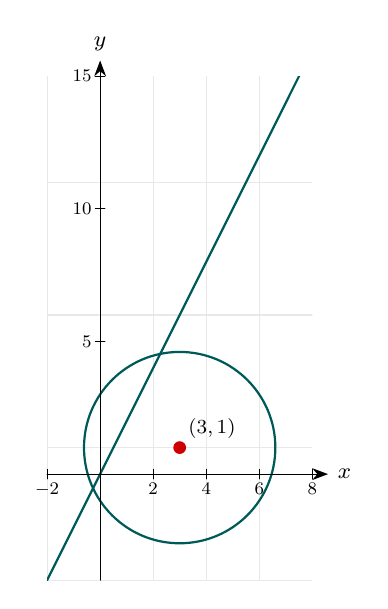
\begin{tikzpicture}[>={Stealth[length=2mm]},font=\footnotesize,line cap=round]
\begin{scope}
\clip (0,0) rectangle (3.368,6.4);
\draw[gray!18] (0,-0.337) grid[xstep=0.674,ystep=1.684] (3.368,6.4);
\draw[teal!70!black,thick] (1.684,1.684) circle (1.215);
\draw[teal!70!black,thick] (0,0) -- (3.368,6.737);
\end{scope}
\draw[->] (0,1.347) -- (3.568,1.347) node[right]{$x$};
\draw[->] (0.674,0) -- (0.674,6.6) node[above]{$y$};
\draw (0,1.287) -- (0,1.407) node[below=2pt,scale=0.8]{$-2$};
\draw (1.347,1.287) -- (1.347,1.407) node[below=2pt,scale=0.8]{$2$};
\draw (2.021,1.287) -- (2.021,1.407) node[below=2pt,scale=0.8]{$4$};
\draw (2.695,1.287) -- (2.695,1.407) node[below=2pt,scale=0.8]{$6$};
\draw (3.368,1.287) -- (3.368,1.407) node[below=2pt,scale=0.8]{$8$};
\draw (0.614,3.032) -- (0.734,3.032) node[left=2pt,scale=0.8]{$5$};
\draw (0.614,4.716) -- (0.734,4.716) node[left=2pt,scale=0.8]{$10$};
\draw (0.614,6.4) -- (0.734,6.4) node[left=2pt,scale=0.8]{$15$};
\fill[red!80!black] (1.684,1.684) circle (2.3pt);
\node[above right,scale=0.9] at (1.684,1.684) {$(3,1)$};
\end{tikzpicture}
}
\end{center}
\small The points and segments shown on the coordinate plane.\normalsize

\medskip\hrule

\section*{Line Segments 40\quad\small\texttt{(cg2-040)}}
\addcontentsline{toc}{section}{Line Segments 40 (cg2-040)}
\textit{Difficulty: Foundation \quad\textbar\quad Marks: 2}

\question{Find the coordinates of the centroid of the triangle with vertices \( (2, 1) \), \( (8, 3) \), \( (5, 8) \).}

\textbf{Worked solution.}

\textit{Centroid formula}
\[\begin{gathered}
G = \left(\frac{2+8+5}{3}, \frac{1+3+8}{3}\right) = (5, 4)
\end{gathered}\]
The centroid is the mean of the three vertices: average all x-coordinates and average all y-coordinates. It is the point where all three medians intersect.

\begin{answerbox}
\textbf{Final answer:}\quad \(\displaystyle (5, 4)\)
\end{answerbox}
\textbf{Diagram.}

\begin{center}
\resizebox{\ifdim\width>\linewidth \linewidth\else \width\fi}{!}{%
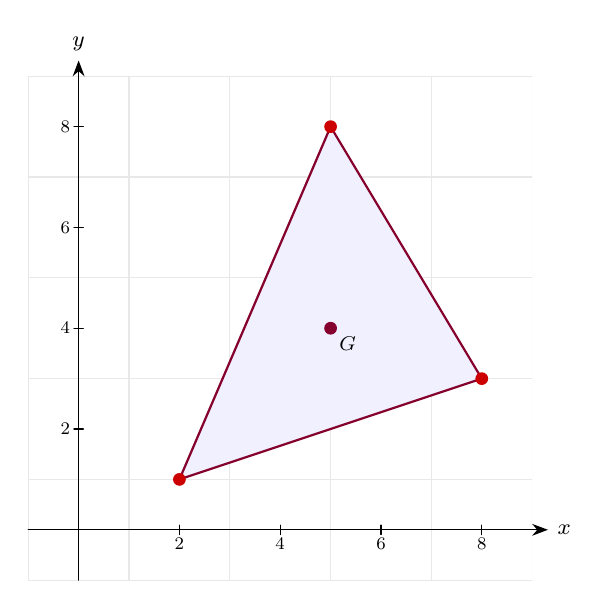
\begin{tikzpicture}[>={Stealth[length=2mm]},font=\footnotesize,line cap=round]
\begin{scope}
\clip (0,0) rectangle (6.4,6.4);
\draw[gray!18] (-0.64,-0.64) grid[xstep=1.28,ystep=1.28] (6.4,6.4);
\fill[blue!6] (1.92,1.28) -- (5.76,2.56) -- (3.84,5.76) -- cycle;
\draw[purple!70!black,thick] (1.92,1.28) -- (5.76,2.56) -- (3.84,5.76) -- cycle;
\end{scope}
\draw[->] (0,0.64) -- (6.6,0.64) node[right]{$x$};
\draw[->] (0.64,0) -- (0.64,6.6) node[above]{$y$};
\draw (1.92,0.58) -- (1.92,0.7) node[below=2pt,scale=0.8]{$2$};
\draw (3.2,0.58) -- (3.2,0.7) node[below=2pt,scale=0.8]{$4$};
\draw (4.48,0.58) -- (4.48,0.7) node[below=2pt,scale=0.8]{$6$};
\draw (5.76,0.58) -- (5.76,0.7) node[below=2pt,scale=0.8]{$8$};
\draw (0.58,1.92) -- (0.7,1.92) node[left=2pt,scale=0.8]{$2$};
\draw (0.58,3.2) -- (0.7,3.2) node[left=2pt,scale=0.8]{$4$};
\draw (0.58,4.48) -- (0.7,4.48) node[left=2pt,scale=0.8]{$6$};
\draw (0.58,5.76) -- (0.7,5.76) node[left=2pt,scale=0.8]{$8$};
\fill[red!80!black] (1.92,1.28) circle (2.3pt);
\fill[red!80!black] (5.76,2.56) circle (2.3pt);
\fill[red!80!black] (3.84,5.76) circle (2.3pt);
\fill[purple!70!black] (3.84,3.2) circle (2.3pt);
\node[below right,scale=0.9] at (3.84,3.2) {$G$};
\end{tikzpicture}
}
\end{center}
\small The points and segments shown on the coordinate plane.\normalsize

\medskip\hrule

\section*{Line Segments 41\quad\small\texttt{(cg2-041)}}
\addcontentsline{toc}{section}{Line Segments 41 (cg2-041)}
\textit{Difficulty: Foundation \quad\textbar\quad Marks: 4}

\question{The points \( A(1, 2) \) and \( B(7, 10) \) are the endpoints of a diameter of a circle. Find the equation of the circle.}

\textbf{Worked solution.}

\textit{Step 1: Centre}
\[\begin{gathered}
C = (4, 6)
\end{gathered}\]
Midpoint of AB.

\textit{Step 2: Radius}
\[\begin{gathered}
r = \frac{1}{2}\sqrt{36+64} = \frac{1}{2}(10) = 5
\end{gathered}\]
The radius is half the diameter length. Find the full distance AB first, then halve it.

\textit{Step 3: Equation}
\[\begin{gathered}
(x-4)^2 + (y-6)^2 = 25
\end{gathered}\]
The standard circle equation is \((x-a)^2 + (y-b)^2 = r^2\), where \((a,b)\) is the centre. Remember to write \(r^2\), not \(r\), on the right side.

\begin{answerbox}
\textbf{Final answer:}\quad \(\displaystyle (x-4)^2 + (y-6)^2 = 25\)
\end{answerbox}
\textbf{Diagram.}

\begin{center}
\resizebox{\ifdim\width>\linewidth \linewidth\else \width\fi}{!}{%
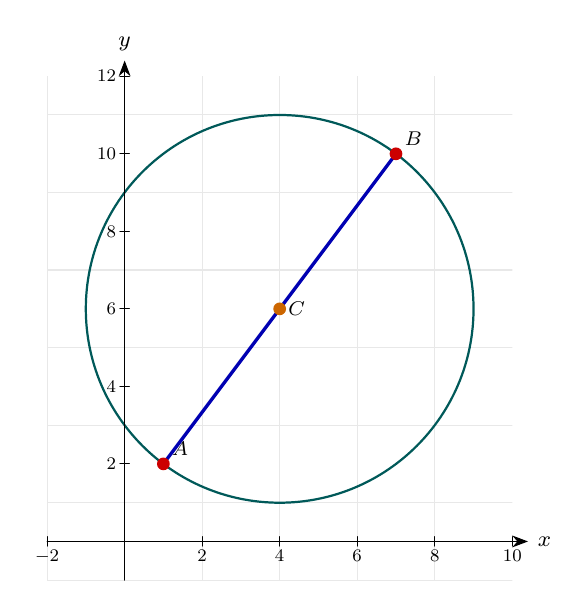
\begin{tikzpicture}[>={Stealth[length=2mm]},font=\footnotesize,line cap=round]
\begin{scope}
\clip (0,0) rectangle (5.908,6.4);
\draw[gray!18] (0,-0.492) grid[xstep=0.985,ystep=0.985] (5.908,6.4);
\draw[teal!70!black,thick] (2.954,3.446) circle (2.462);
\draw[blue!70!black,very thick] (1.477,1.477) -- (4.431,5.415);
\end{scope}
\draw[->] (0,0.492) -- (6.108,0.492) node[right]{$x$};
\draw[->] (0.985,0) -- (0.985,6.6) node[above]{$y$};
\draw (0,0.432) -- (0,0.552) node[below=2pt,scale=0.8]{$-2$};
\draw (1.969,0.432) -- (1.969,0.552) node[below=2pt,scale=0.8]{$2$};
\draw (2.954,0.432) -- (2.954,0.552) node[below=2pt,scale=0.8]{$4$};
\draw (3.938,0.432) -- (3.938,0.552) node[below=2pt,scale=0.8]{$6$};
\draw (4.923,0.432) -- (4.923,0.552) node[below=2pt,scale=0.8]{$8$};
\draw (5.908,0.432) -- (5.908,0.552) node[below=2pt,scale=0.8]{$10$};
\draw (0.925,1.477) -- (1.045,1.477) node[left=2pt,scale=0.8]{$2$};
\draw (0.925,2.462) -- (1.045,2.462) node[left=2pt,scale=0.8]{$4$};
\draw (0.925,3.446) -- (1.045,3.446) node[left=2pt,scale=0.8]{$6$};
\draw (0.925,4.431) -- (1.045,4.431) node[left=2pt,scale=0.8]{$8$};
\draw (0.925,5.415) -- (1.045,5.415) node[left=2pt,scale=0.8]{$10$};
\draw (0.925,6.4) -- (1.045,6.4) node[left=2pt,scale=0.8]{$12$};
\fill[red!80!black] (1.477,1.477) circle (2.3pt);
\node[above right,scale=0.9] at (1.477,1.477) {$A$};
\fill[red!80!black] (4.431,5.415) circle (2.3pt);
\node[above right,scale=0.9] at (4.431,5.415) {$B$};
\fill[orange!80!black] (2.954,3.446) circle (2.3pt);
\node[right,scale=0.9] at (2.954,3.446) {$C$};
\end{tikzpicture}
}
\end{center}
\small The points and segments shown on the coordinate plane.\normalsize

\medskip\hrule

\section*{Line Segments 42\quad\small\texttt{(cg2-042)}}
\addcontentsline{toc}{section}{Line Segments 42 (cg2-042)}
\textit{Difficulty: Foundation \quad\textbar\quad Marks: 3}

\question{Find the distance between the parallel lines \( y = 2x + 1 \) and \( y = 2x + 6 \).}

\textbf{Worked solution.}

\textit{Step 1: Rewrite as ax + by + c = 0}
\[\begin{gathered}
2x - y + 1 = 0 \text{ and } 2x - y + 6 = 0
\end{gathered}\]
Both lines must be in the form \(ax + by + c = 0\) with the same \(a\) and \(b\) values to use the parallel lines distance formula.

\textit{Step 2: Distance between parallel lines}
\[\begin{gathered}
d = \frac{|6-1|}{\sqrt{4+1}} = \frac{5}{\sqrt{5}} = \sqrt{5}
\end{gathered}\]
The formula for distance between parallel lines \(ax+by+c_1=0\) and \(ax+by+c_2=0\) is \(\frac{|c_2 - c_1|}{\sqrt{a^2+b^2}}\). Rationalise: \(\frac{5}{\sqrt{5}} = \sqrt{5}\).

\begin{answerbox}
\textbf{Final answer:}\quad \(\displaystyle \sqrt{5}\)
\end{answerbox}
\textbf{Diagram.}

\begin{center}
\resizebox{\ifdim\width>\linewidth \linewidth\else \width\fi}{!}{%
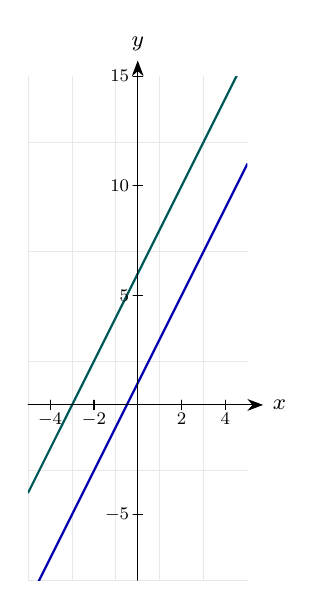
\begin{tikzpicture}[>={Stealth[length=2mm]},font=\footnotesize,line cap=round]
\begin{scope}
\clip (0,0) rectangle (2.783,6.4);
\draw[gray!18] (-0.278,-0.557) grid[xstep=0.557,ystep=1.391] (2.783,6.4);
\draw[blue!70!black,thick] (0,-0.278) -- (2.783,5.287);
\draw[teal!70!black,thick] (0,1.113) -- (2.783,6.678);
\end{scope}
\draw[->] (0,2.226) -- (2.983,2.226) node[right]{$x$};
\draw[->] (1.391,0) -- (1.391,6.6) node[above]{$y$};
\draw (0.278,2.166) -- (0.278,2.286) node[below=2pt,scale=0.8]{$-4$};
\draw (0.835,2.166) -- (0.835,2.286) node[below=2pt,scale=0.8]{$-2$};
\draw (1.948,2.166) -- (1.948,2.286) node[below=2pt,scale=0.8]{$2$};
\draw (2.504,2.166) -- (2.504,2.286) node[below=2pt,scale=0.8]{$4$};
\draw (1.331,0.835) -- (1.451,0.835) node[left=2pt,scale=0.8]{$-5$};
\draw (1.331,3.617) -- (1.451,3.617) node[left=2pt,scale=0.8]{$5$};
\draw (1.331,5.009) -- (1.451,5.009) node[left=2pt,scale=0.8]{$10$};
\draw (1.331,6.4) -- (1.451,6.4) node[left=2pt,scale=0.8]{$15$};
\end{tikzpicture}
}
\end{center}
\small The points and segments shown on the coordinate plane.\normalsize

\medskip\hrule

\section*{Line Segments 43\quad\small\texttt{(cg2-043)}}
\addcontentsline{toc}{section}{Line Segments 43 (cg2-043)}
\textit{Difficulty: Foundation \quad\textbar\quad Marks: 3}

\question{A quadrilateral has vertices \( A(0, 0) \), \( B(5, 0) \), \( C(7, 4) \), \( D(2, 4) \). Find the lengths of its diagonals.}

\textbf{Worked solution.}

\textit{Step 1: Diagonal AC}
\[\begin{gathered}
AC = \sqrt{49+16} = \sqrt{65}
\end{gathered}\]
Distance from A(0,0) to C(7,4). Since 65 has no perfect square factors other than 1, \(\sqrt{65}\) is already in simplest surd form.

\textit{Step 2: Diagonal BD}
\[\begin{gathered}
BD = \sqrt{9+16} = 5
\end{gathered}\]
Distance from B(5,0) to D(2,4). This is a 3-4-5 Pythagorean triple.

\begin{answerbox}
\textbf{Final answer:}\quad \(\displaystyle AC = \sqrt{65}\), \(\displaystyle BD = 5\)
\end{answerbox}
\textbf{Diagram.}

\begin{center}
\resizebox{\ifdim\width>\linewidth \linewidth\else \width\fi}{!}{%
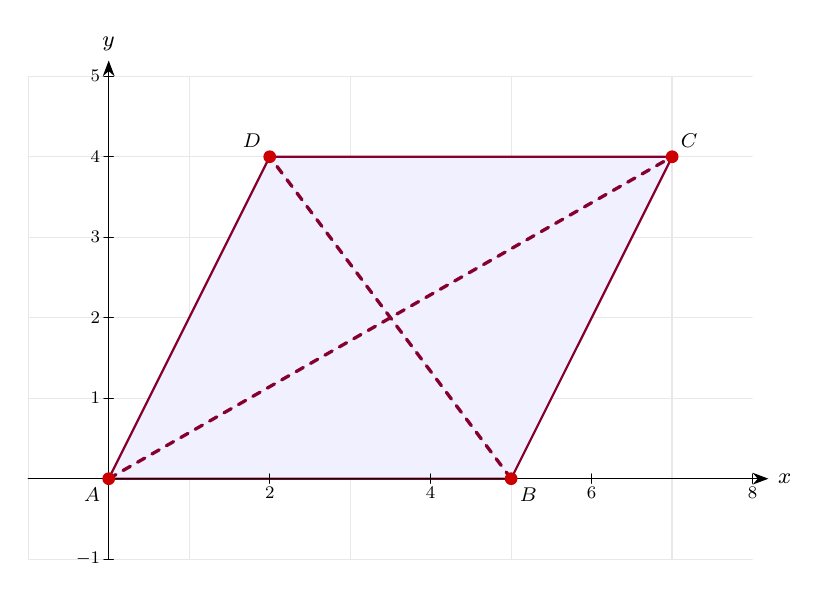
\begin{tikzpicture}[>={Stealth[length=2mm]},font=\footnotesize,line cap=round]
\begin{scope}
\clip (0,0) rectangle (9.2,6.133);
\draw[gray!18] (-1.022,0) grid[xstep=2.044,ystep=1.022] (9.2,6.133);
\fill[blue!6] (1.022,1.022) -- (6.133,1.022) -- (8.178,5.111) -- (3.067,5.111) -- cycle;
\draw[purple!70!black,thick] (1.022,1.022) -- (6.133,1.022) -- (8.178,5.111) -- (3.067,5.111) -- cycle;
\draw[dashed,purple!70!black,very thick] (1.022,1.022) -- (8.178,5.111);
\draw[dashed,purple!70!black,very thick] (6.133,1.022) -- (3.067,5.111);
\end{scope}
\draw[->] (0,1.022) -- (9.4,1.022) node[right]{$x$};
\draw[->] (1.022,0) -- (1.022,6.333) node[above]{$y$};
\draw (3.067,0.962) -- (3.067,1.082) node[below=2pt,scale=0.8]{$2$};
\draw (5.111,0.962) -- (5.111,1.082) node[below=2pt,scale=0.8]{$4$};
\draw (7.156,0.962) -- (7.156,1.082) node[below=2pt,scale=0.8]{$6$};
\draw (9.2,0.962) -- (9.2,1.082) node[below=2pt,scale=0.8]{$8$};
\draw (0.962,0) -- (1.082,0) node[left=2pt,scale=0.8]{$-1$};
\draw (0.962,2.044) -- (1.082,2.044) node[left=2pt,scale=0.8]{$1$};
\draw (0.962,3.067) -- (1.082,3.067) node[left=2pt,scale=0.8]{$2$};
\draw (0.962,4.089) -- (1.082,4.089) node[left=2pt,scale=0.8]{$3$};
\draw (0.962,5.111) -- (1.082,5.111) node[left=2pt,scale=0.8]{$4$};
\draw (0.962,6.133) -- (1.082,6.133) node[left=2pt,scale=0.8]{$5$};
\fill[red!80!black] (1.022,1.022) circle (2.3pt);
\node[below left,scale=0.9] at (1.022,1.022) {$A$};
\fill[red!80!black] (6.133,1.022) circle (2.3pt);
\node[below right,scale=0.9] at (6.133,1.022) {$B$};
\fill[red!80!black] (8.178,5.111) circle (2.3pt);
\node[above right,scale=0.9] at (8.178,5.111) {$C$};
\fill[red!80!black] (3.067,5.111) circle (2.3pt);
\node[above left,scale=0.9] at (3.067,5.111) {$D$};
\end{tikzpicture}
}
\end{center}
\small The points and segments shown on the coordinate plane.\normalsize

\medskip\hrule

\section*{Line Segments 44\quad\small\texttt{(cg2-044)}}
\addcontentsline{toc}{section}{Line Segments 44 (cg2-044)}
\textit{Difficulty: Foundation \quad\textbar\quad Marks: 3}

\question{The point \( P \) divides \( AB \) externally in the ratio \( 3:1 \), where \( A = (2, 4) \) and \( B = (6, 8) \). Find \( P \).}

\textbf{Worked solution.}

\textit{External division formula}
\[\begin{gathered}
P = \left(\frac{3(6)-1(2)}{3-1}, \frac{3(8)-1(4)}{3-1}\right) = (8, 10)
\end{gathered}\]
For external division in ratio \(m:n\), use the formula \(P = \left(\frac{mx_2 - nx_1}{m-n}, \frac{my_2 - ny_1}{m-n}\right)\). Note the minus signs --- this is the key difference from internal division.

\begin{answerbox}
\textbf{Final answer:}\quad \(\displaystyle (8, 10)\)
\end{answerbox}
\textbf{Diagram.}

\begin{center}
\resizebox{\ifdim\width>\linewidth \linewidth\else \width\fi}{!}{%
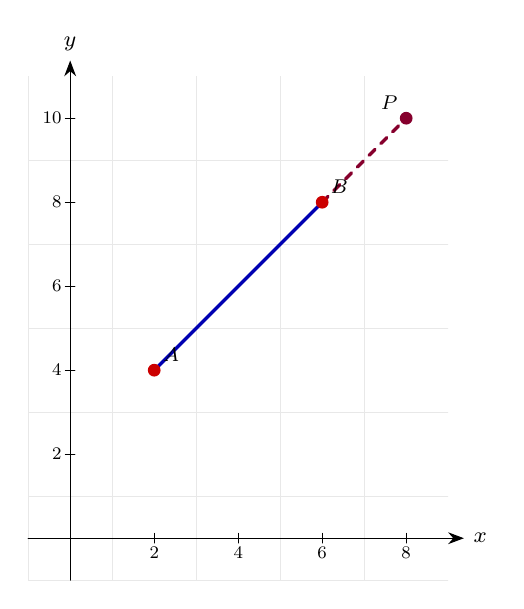
\begin{tikzpicture}[>={Stealth[length=2mm]},font=\footnotesize,line cap=round]
\begin{scope}
\clip (0,0) rectangle (5.333,6.4);
\draw[gray!18] (-0.533,-0.533) grid[xstep=1.067,ystep=1.067] (5.333,6.4);
\draw[blue!70!black,very thick] (1.6,2.667) -- (3.733,4.8);
\draw[dashed,purple!70!black,very thick] (3.733,4.8) -- (4.8,5.867);
\end{scope}
\draw[->] (0,0.533) -- (5.533,0.533) node[right]{$x$};
\draw[->] (0.533,0) -- (0.533,6.6) node[above]{$y$};
\draw (1.6,0.473) -- (1.6,0.593) node[below=2pt,scale=0.8]{$2$};
\draw (2.667,0.473) -- (2.667,0.593) node[below=2pt,scale=0.8]{$4$};
\draw (3.733,0.473) -- (3.733,0.593) node[below=2pt,scale=0.8]{$6$};
\draw (4.8,0.473) -- (4.8,0.593) node[below=2pt,scale=0.8]{$8$};
\draw (0.473,1.6) -- (0.593,1.6) node[left=2pt,scale=0.8]{$2$};
\draw (0.473,2.667) -- (0.593,2.667) node[left=2pt,scale=0.8]{$4$};
\draw (0.473,3.733) -- (0.593,3.733) node[left=2pt,scale=0.8]{$6$};
\draw (0.473,4.8) -- (0.593,4.8) node[left=2pt,scale=0.8]{$8$};
\draw (0.473,5.867) -- (0.593,5.867) node[left=2pt,scale=0.8]{$10$};
\fill[red!80!black] (1.6,2.667) circle (2.3pt);
\node[above right,scale=0.9] at (1.6,2.667) {$A$};
\fill[red!80!black] (3.733,4.8) circle (2.3pt);
\node[above right,scale=0.9] at (3.733,4.8) {$B$};
\fill[purple!70!black] (4.8,5.867) circle (2.3pt);
\node[above left,scale=0.9] at (4.8,5.867) {$P$};
\end{tikzpicture}
}
\end{center}
\small The points and segments shown on the coordinate plane.\normalsize

\medskip\hrule

\section*{Line Segments 45\quad\small\texttt{(cg2-045)}}
\addcontentsline{toc}{section}{Line Segments 45 (cg2-045)}
\textit{Difficulty: Foundation \quad\textbar\quad Marks: 2}

\question{The midpoint of \( AB \) is \( (0, 0) \). If \( A = (3a, -2b) \), express \( B \) in terms of \( a \) and \( b \).}

\textbf{Worked solution.}

\textit{Use midpoint = (0,0)}
\[\begin{gathered}
B = (-3a, 2b)
\end{gathered}\]
Since midpoint is origin, B is the negative of A.

\begin{answerbox}
\textbf{Final answer:}\quad \(\displaystyle B = (-3a, 2b)\)
\end{answerbox}
\textbf{Diagram.}

\begin{center}
\resizebox{\ifdim\width>\linewidth \linewidth\else \width\fi}{!}{%
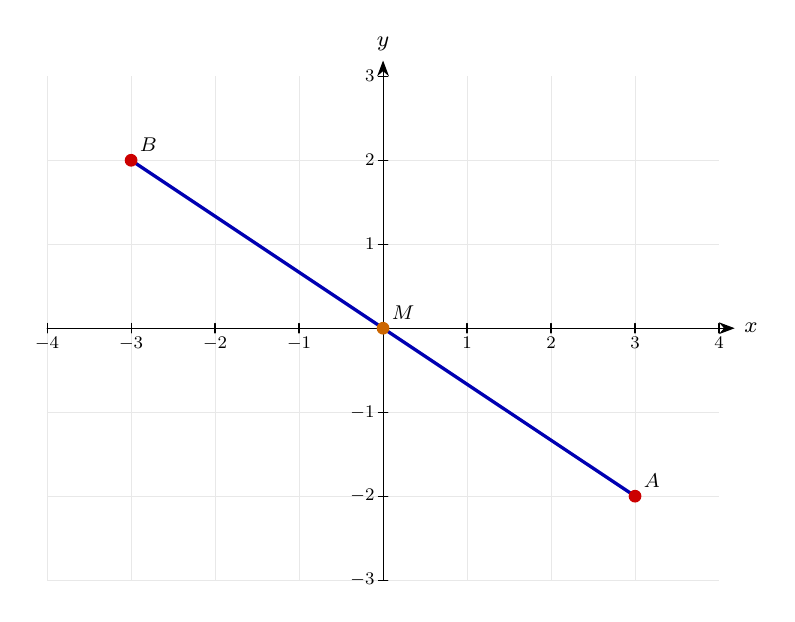
\begin{tikzpicture}[>={Stealth[length=2mm]},font=\footnotesize,line cap=round]
\begin{scope}
\clip (0,0) rectangle (8.533,6.4);
\draw[gray!18] (0,0) grid[xstep=1.067,ystep=1.067] (8.533,6.4);
\draw[blue!70!black,very thick] (7.467,1.067) -- (1.067,5.333);
\end{scope}
\draw[->] (0,3.2) -- (8.733,3.2) node[right]{$x$};
\draw[->] (4.267,0) -- (4.267,6.6) node[above]{$y$};
\draw (0,3.14) -- (0,3.26) node[below=2pt,scale=0.8]{$-4$};
\draw (1.067,3.14) -- (1.067,3.26) node[below=2pt,scale=0.8]{$-3$};
\draw (2.133,3.14) -- (2.133,3.26) node[below=2pt,scale=0.8]{$-2$};
\draw (3.2,3.14) -- (3.2,3.26) node[below=2pt,scale=0.8]{$-1$};
\draw (5.333,3.14) -- (5.333,3.26) node[below=2pt,scale=0.8]{$1$};
\draw (6.4,3.14) -- (6.4,3.26) node[below=2pt,scale=0.8]{$2$};
\draw (7.467,3.14) -- (7.467,3.26) node[below=2pt,scale=0.8]{$3$};
\draw (8.533,3.14) -- (8.533,3.26) node[below=2pt,scale=0.8]{$4$};
\draw (4.207,0) -- (4.327,0) node[left=2pt,scale=0.8]{$-3$};
\draw (4.207,1.067) -- (4.327,1.067) node[left=2pt,scale=0.8]{$-2$};
\draw (4.207,2.133) -- (4.327,2.133) node[left=2pt,scale=0.8]{$-1$};
\draw (4.207,4.267) -- (4.327,4.267) node[left=2pt,scale=0.8]{$1$};
\draw (4.207,5.333) -- (4.327,5.333) node[left=2pt,scale=0.8]{$2$};
\draw (4.207,6.4) -- (4.327,6.4) node[left=2pt,scale=0.8]{$3$};
\fill[red!80!black] (7.467,1.067) circle (2.3pt);
\node[above right,scale=0.9] at (7.467,1.067) {$A$};
\fill[red!80!black] (1.067,5.333) circle (2.3pt);
\node[above right,scale=0.9] at (1.067,5.333) {$B$};
\fill[orange!80!black] (4.267,3.2) circle (2.3pt);
\node[above right,scale=0.9] at (4.267,3.2) {$M$};
\end{tikzpicture}
}
\end{center}
\small The points and segments shown on the coordinate plane.\normalsize

\medskip\hrule

\section*{Line Segments 46\quad\small\texttt{(cg2-046)}}
\addcontentsline{toc}{section}{Line Segments 46 (cg2-046)}
\textit{Difficulty: Foundation \quad\textbar\quad Marks: 2}

\question{Find the area of the triangle with vertices \( (0, 0) \), \( (6, 0) \), \( (3, 8) \).}

\textbf{Worked solution.}

\textit{Area formula}
\[\begin{gathered}
\text{Area} = \frac{1}{2} \times 6 \times 8 = 24
\end{gathered}\]
Base = 6 along x-axis, height = 8.

\begin{answerbox}
\textbf{Final answer:}\quad \(\displaystyle 24\) square units
\end{answerbox}
\textbf{Diagram.}

\begin{center}
\resizebox{\ifdim\width>\linewidth \linewidth\else \width\fi}{!}{%
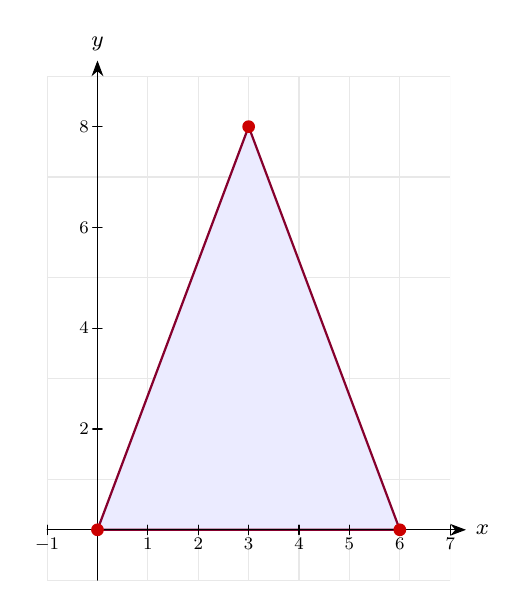
\begin{tikzpicture}[>={Stealth[length=2mm]},font=\footnotesize,line cap=round]
\begin{scope}
\clip (0,0) rectangle (5.12,6.4);
\draw[gray!18] (0,-0.64) grid[xstep=0.64,ystep=1.28] (5.12,6.4);
\fill[blue!8] (0.64,0.64) -- (4.48,0.64) -- (2.56,5.76) -- cycle;
\draw[purple!70!black,thick] (0.64,0.64) -- (4.48,0.64) -- (2.56,5.76) -- cycle;
\end{scope}
\draw[->] (0,0.64) -- (5.32,0.64) node[right]{$x$};
\draw[->] (0.64,0) -- (0.64,6.6) node[above]{$y$};
\draw (0,0.58) -- (0,0.7) node[below=2pt,scale=0.8]{$-1$};
\draw (1.28,0.58) -- (1.28,0.7) node[below=2pt,scale=0.8]{$1$};
\draw (1.92,0.58) -- (1.92,0.7) node[below=2pt,scale=0.8]{$2$};
\draw (2.56,0.58) -- (2.56,0.7) node[below=2pt,scale=0.8]{$3$};
\draw (3.2,0.58) -- (3.2,0.7) node[below=2pt,scale=0.8]{$4$};
\draw (3.84,0.58) -- (3.84,0.7) node[below=2pt,scale=0.8]{$5$};
\draw (4.48,0.58) -- (4.48,0.7) node[below=2pt,scale=0.8]{$6$};
\draw (5.12,0.58) -- (5.12,0.7) node[below=2pt,scale=0.8]{$7$};
\draw (0.58,1.92) -- (0.7,1.92) node[left=2pt,scale=0.8]{$2$};
\draw (0.58,3.2) -- (0.7,3.2) node[left=2pt,scale=0.8]{$4$};
\draw (0.58,4.48) -- (0.7,4.48) node[left=2pt,scale=0.8]{$6$};
\draw (0.58,5.76) -- (0.7,5.76) node[left=2pt,scale=0.8]{$8$};
\fill[red!80!black] (0.64,0.64) circle (2.3pt);
\fill[red!80!black] (4.48,0.64) circle (2.3pt);
\fill[red!80!black] (2.56,5.76) circle (2.3pt);
\end{tikzpicture}
}
\end{center}
\small The points and segments shown on the coordinate plane.\normalsize

\medskip\hrule

\section*{Line Segments 47\quad\small\texttt{(cg2-047)}}
\addcontentsline{toc}{section}{Line Segments 47 (cg2-047)}
\textit{Difficulty: Foundation \quad\textbar\quad Marks: 5}

\question{Show that \( A(-1, 2) \), \( B(3, 0) \), \( C(5, 4) \), \( D(1, 6) \) form a square.}

\textbf{Worked solution.}

\textit{Step 1: Find all side lengths}
\[\begin{gathered}
AB = \sqrt{16+4} = \sqrt{20}, \quad BC = \sqrt{4+16} = \sqrt{20}
\end{gathered}\]
Apply the distance formula to each pair of consecutive vertices. To show a square, we need all four sides equal and at least one right angle.

\textit{Step 2: Remaining sides}
\[\begin{gathered}
CD = \sqrt{16+4} = \sqrt{20}, \quad DA = \sqrt{4+16} = \sqrt{20}
\end{gathered}\]
All sides equal.

\textit{Step 3: Check right angle}
\[\begin{gathered}
m_{AB} = -\frac{1}{2}, \quad m_{BC} = 2; \quad m_{AB} \times m_{BC} = -1 \checkmark
\end{gathered}\]
Perpendicular adjacent sides.

\begin{answerbox}
\textbf{Final answer:}\quad All sides \(\displaystyle \sqrt{20}\) and adjacent sides perpendicular, so ABCD is a square.
\end{answerbox}
\textbf{Diagram.}

\begin{center}
\resizebox{\ifdim\width>\linewidth \linewidth\else \width\fi}{!}{%
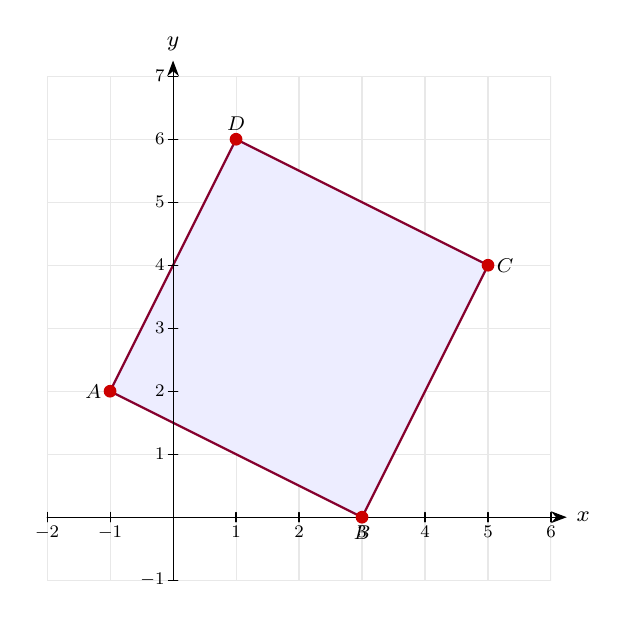
\begin{tikzpicture}[>={Stealth[length=2mm]},font=\footnotesize,line cap=round]
\begin{scope}
\clip (0,0) rectangle (6.4,6.4);
\draw[gray!18] (0,0) grid[xstep=0.8,ystep=0.8] (6.4,6.4);
\fill[blue!7] (0.8,2.4) -- (4,0.8) -- (5.6,4) -- (2.4,5.6) -- cycle;
\draw[purple!70!black,thick] (0.8,2.4) -- (4,0.8) -- (5.6,4) -- (2.4,5.6) -- cycle;
\end{scope}
\draw[->] (0,0.8) -- (6.6,0.8) node[right]{$x$};
\draw[->] (1.6,0) -- (1.6,6.6) node[above]{$y$};
\draw (0,0.74) -- (0,0.86) node[below=2pt,scale=0.8]{$-2$};
\draw (0.8,0.74) -- (0.8,0.86) node[below=2pt,scale=0.8]{$-1$};
\draw (2.4,0.74) -- (2.4,0.86) node[below=2pt,scale=0.8]{$1$};
\draw (3.2,0.74) -- (3.2,0.86) node[below=2pt,scale=0.8]{$2$};
\draw (4,0.74) -- (4,0.86) node[below=2pt,scale=0.8]{$3$};
\draw (4.8,0.74) -- (4.8,0.86) node[below=2pt,scale=0.8]{$4$};
\draw (5.6,0.74) -- (5.6,0.86) node[below=2pt,scale=0.8]{$5$};
\draw (6.4,0.74) -- (6.4,0.86) node[below=2pt,scale=0.8]{$6$};
\draw (1.54,0) -- (1.66,0) node[left=2pt,scale=0.8]{$-1$};
\draw (1.54,1.6) -- (1.66,1.6) node[left=2pt,scale=0.8]{$1$};
\draw (1.54,2.4) -- (1.66,2.4) node[left=2pt,scale=0.8]{$2$};
\draw (1.54,3.2) -- (1.66,3.2) node[left=2pt,scale=0.8]{$3$};
\draw (1.54,4) -- (1.66,4) node[left=2pt,scale=0.8]{$4$};
\draw (1.54,4.8) -- (1.66,4.8) node[left=2pt,scale=0.8]{$5$};
\draw (1.54,5.6) -- (1.66,5.6) node[left=2pt,scale=0.8]{$6$};
\draw (1.54,6.4) -- (1.66,6.4) node[left=2pt,scale=0.8]{$7$};
\fill[red!80!black] (0.8,2.4) circle (2.3pt);
\node[left,scale=0.9] at (0.8,2.4) {$A$};
\fill[red!80!black] (4,0.8) circle (2.3pt);
\node[below,scale=0.9] at (4,0.8) {$B$};
\fill[red!80!black] (5.6,4) circle (2.3pt);
\node[right,scale=0.9] at (5.6,4) {$C$};
\fill[red!80!black] (2.4,5.6) circle (2.3pt);
\node[above,scale=0.9] at (2.4,5.6) {$D$};
\end{tikzpicture}
}
\end{center}
\small The points and segments shown on the coordinate plane.\normalsize

\medskip\hrule

\section*{Line Segments 48\quad\small\texttt{(cg2-048)}}
\addcontentsline{toc}{section}{Line Segments 48 (cg2-048)}
\textit{Difficulty: Foundation \quad\textbar\quad Marks: 3}

\question{Find the length of the line segment from \( (\cos\theta, \sin\theta) \) to \( (-\cos\theta, -\sin\theta) \).}

\textbf{Worked solution.}

\textit{Distance formula}
\[\begin{gathered}
d = \sqrt{(2\cos\theta)^2 + (2\sin\theta)^2} = 2\sqrt{\cos^2\theta + \sin^2\theta} = 2
\end{gathered}\]
Using the Pythagorean identity.

\begin{answerbox}
\textbf{Final answer:}\quad \(\displaystyle 2\)
\end{answerbox}
\textbf{Diagram.}

\begin{center}
\resizebox{\ifdim\width>\linewidth \linewidth\else \width\fi}{!}{%
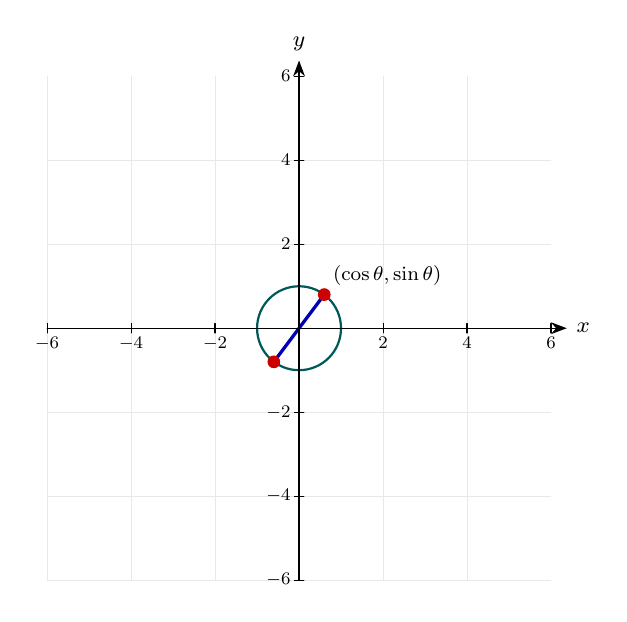
\begin{tikzpicture}[>={Stealth[length=2mm]},font=\footnotesize,line cap=round]
\begin{scope}
\clip (0,0) rectangle (6.4,6.4);
\draw[gray!18] (0,0) grid[xstep=1.067,ystep=1.067] (6.4,6.4);
\draw[teal!70!black,thick] (3.2,3.2) circle (0.533);
\draw[blue!70!black,very thick] (3.52,3.627) -- (2.88,2.773);
\end{scope}
\draw[->] (0,3.2) -- (6.6,3.2) node[right]{$x$};
\draw[->] (3.2,0) -- (3.2,6.6) node[above]{$y$};
\draw (0,3.14) -- (0,3.26) node[below=2pt,scale=0.8]{$-6$};
\draw (1.067,3.14) -- (1.067,3.26) node[below=2pt,scale=0.8]{$-4$};
\draw (2.133,3.14) -- (2.133,3.26) node[below=2pt,scale=0.8]{$-2$};
\draw (4.267,3.14) -- (4.267,3.26) node[below=2pt,scale=0.8]{$2$};
\draw (5.333,3.14) -- (5.333,3.26) node[below=2pt,scale=0.8]{$4$};
\draw (6.4,3.14) -- (6.4,3.26) node[below=2pt,scale=0.8]{$6$};
\draw (3.14,0) -- (3.26,0) node[left=2pt,scale=0.8]{$-6$};
\draw (3.14,1.067) -- (3.26,1.067) node[left=2pt,scale=0.8]{$-4$};
\draw (3.14,2.133) -- (3.26,2.133) node[left=2pt,scale=0.8]{$-2$};
\draw (3.14,4.267) -- (3.26,4.267) node[left=2pt,scale=0.8]{$2$};
\draw (3.14,5.333) -- (3.26,5.333) node[left=2pt,scale=0.8]{$4$};
\draw (3.14,6.4) -- (3.26,6.4) node[left=2pt,scale=0.8]{$6$};
\fill[red!80!black] (3.52,3.627) circle (2.3pt);
\node[above right,scale=0.9] at (3.52,3.627) {$(\cos\theta,\sin\theta)$};
\fill[red!80!black] (2.88,2.773) circle (2.3pt);
\end{tikzpicture}
}
\end{center}
\small The points and segments shown on the coordinate plane.\normalsize

\medskip\hrule

\section*{Line Segments 49\quad\small\texttt{(cg2-049)}}
\addcontentsline{toc}{section}{Line Segments 49 (cg2-049)}
\textit{Difficulty: Foundation \quad\textbar\quad Marks: 4}

\question{The line segment \( AB \) has length 10. \( A = (1, 2) \) and \( B \) lies on the x-axis. Find the possible coordinates of \( B \).}

\textbf{Worked solution.}

\textit{Step 1: Let B = (x, 0)}
\[\begin{gathered}
(x-1)^2 + 4 = 100 \implies (x-1)^2 = 96
\end{gathered}\]
Since B is on the x-axis, its y-coordinate is 0. Substitute into the distance formula squared: \((x-1)^2 + (0-2)^2 = 10^2\).

\textit{Step 2: Solve}
\[\begin{gathered}
x = 1 \pm 4\sqrt{6}
\end{gathered}\]
Take the square root of both sides: \(\sqrt{96} = \sqrt{16 \times 6} = 4\sqrt{6}\). Two solutions arise since B could be on either side of A.

\begin{answerbox}
\textbf{Final answer:}\quad \(\displaystyle B = (1 + 4\sqrt{6}, 0)\) or \(\displaystyle B = (1 - 4\sqrt{6}, 0)\)
\end{answerbox}
\textbf{Diagram.}

\begin{center}
\resizebox{\ifdim\width>\linewidth \linewidth\else \width\fi}{!}{%
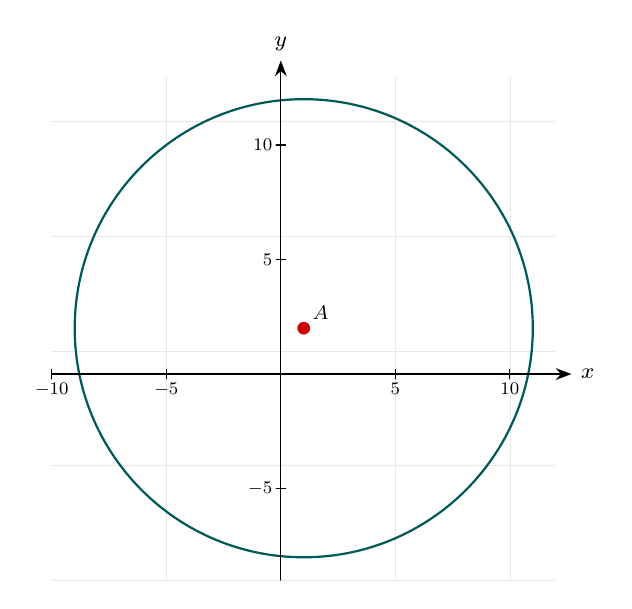
\begin{tikzpicture}[>={Stealth[length=2mm]},font=\footnotesize,line cap=round]
\begin{scope}
\clip (0,0) rectangle (6.4,6.4);
\draw[gray!18] (0,-0.291) grid[xstep=1.455,ystep=1.455] (6.4,6.4);
\draw[teal!70!black,thick] (3.2,3.2) circle (2.909);
\draw[gray,thick] (0,2.618) -- (6.4,2.618);
\end{scope}
\draw[->] (0,2.618) -- (6.6,2.618) node[right]{$x$};
\draw[->] (2.909,0) -- (2.909,6.6) node[above]{$y$};
\draw (0,2.558) -- (0,2.678) node[below=2pt,scale=0.8]{$-10$};
\draw (1.455,2.558) -- (1.455,2.678) node[below=2pt,scale=0.8]{$-5$};
\draw (4.364,2.558) -- (4.364,2.678) node[below=2pt,scale=0.8]{$5$};
\draw (5.818,2.558) -- (5.818,2.678) node[below=2pt,scale=0.8]{$10$};
\draw (2.849,1.164) -- (2.969,1.164) node[left=2pt,scale=0.8]{$-5$};
\draw (2.849,4.073) -- (2.969,4.073) node[left=2pt,scale=0.8]{$5$};
\draw (2.849,5.527) -- (2.969,5.527) node[left=2pt,scale=0.8]{$10$};
\fill[red!80!black] (3.2,3.2) circle (2.3pt);
\node[above right,scale=0.9] at (3.2,3.2) {$A$};
\end{tikzpicture}
}
\end{center}
\small The points and segments shown on the coordinate plane.\normalsize

\medskip\hrule

\section*{Line Segments 50\quad\small\texttt{(cg2-050)}}
\addcontentsline{toc}{section}{Line Segments 50 (cg2-050)}
\textit{Difficulty: Foundation \quad\textbar\quad Marks: 7}

\question{A triangle has vertices \( P(2, 1) \), \( Q(8, 1) \), \( R(5, 7) \). Find: (a) the perimeter; (b) the area; (c) the coordinates of the centroid.}

\textbf{Worked solution.}

\textit{Step 1: (a) Side lengths}
\[\begin{gathered}
PQ = 6, \quad PR = \sqrt{9+36} = \sqrt{45} = 3\sqrt{5}, \quad QR = \sqrt{9+36} = 3\sqrt{5}
\end{gathered}\]
PQ is horizontal (same y-coordinate), so its length is simply |8 - 2| = 6. Simplify surds: sqrt(45) = sqrt(9 x 5) = 3sqrt(5).

\textit{Step 2: Perimeter}
\[\begin{gathered}
P = 6 + 6\sqrt{5} \approx 19.42
\end{gathered}\]
Sum all three sides: 6 + 3sqrt(5) + 3sqrt(5) = 6 + 6sqrt(5). Collect like surds before adding.

\textit{Step 3: (b) Area}
\[\begin{gathered}
\text{Area} = \frac{1}{2} \times 6 \times 6 = 18
\end{gathered}\]
Base PQ = 6, height = 7 - 1 = 6.

\textit{Step 4: (c) Centroid}
\[\begin{gathered}
G = \left(\frac{2+8+5}{3}, \frac{1+1+7}{3}\right) = (5, 3)
\end{gathered}\]
The centroid is the average of the three vertices: add all x-coordinates and divide by 3, then do the same for y-coordinates.

\begin{answerbox}
\textbf{Final answer:}\quad (a) \(\displaystyle 6 + 6\sqrt{5}\); (b) \(\displaystyle 18\); (c) \(\displaystyle (5, 3)\)
\end{answerbox}
\textbf{Diagram.}

\begin{center}
\resizebox{\ifdim\width>\linewidth \linewidth\else \width\fi}{!}{%
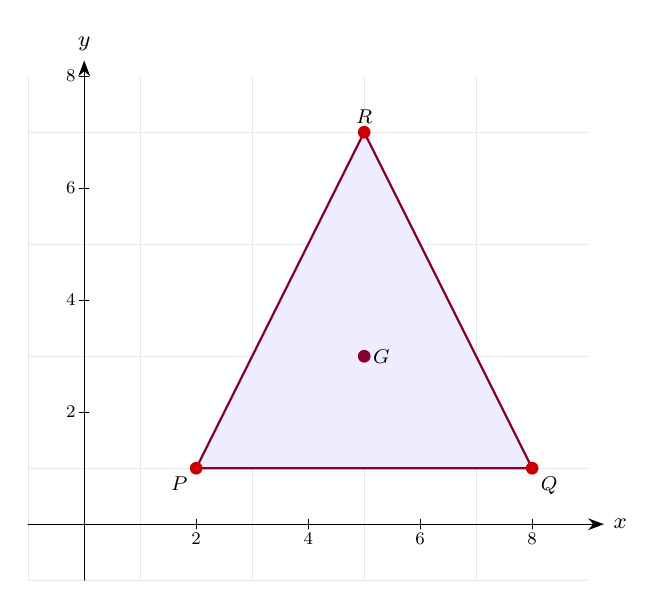
\begin{tikzpicture}[>={Stealth[length=2mm]},font=\footnotesize,line cap=round]
\begin{scope}
\clip (0,0) rectangle (7.111,6.4);
\draw[gray!18] (-0.711,-0.711) grid[xstep=1.422,ystep=1.422] (7.111,6.4);
\fill[blue!7] (2.133,1.422) -- (6.4,1.422) -- (4.267,5.689) -- cycle;
\draw[purple!70!black,thick] (2.133,1.422) -- (6.4,1.422) -- (4.267,5.689) -- cycle;
\end{scope}
\draw[->] (0,0.711) -- (7.311,0.711) node[right]{$x$};
\draw[->] (0.711,0) -- (0.711,6.6) node[above]{$y$};
\draw (2.133,0.651) -- (2.133,0.771) node[below=2pt,scale=0.8]{$2$};
\draw (3.556,0.651) -- (3.556,0.771) node[below=2pt,scale=0.8]{$4$};
\draw (4.978,0.651) -- (4.978,0.771) node[below=2pt,scale=0.8]{$6$};
\draw (6.4,0.651) -- (6.4,0.771) node[below=2pt,scale=0.8]{$8$};
\draw (0.651,2.133) -- (0.771,2.133) node[left=2pt,scale=0.8]{$2$};
\draw (0.651,3.556) -- (0.771,3.556) node[left=2pt,scale=0.8]{$4$};
\draw (0.651,4.978) -- (0.771,4.978) node[left=2pt,scale=0.8]{$6$};
\draw (0.651,6.4) -- (0.771,6.4) node[left=2pt,scale=0.8]{$8$};
\fill[red!80!black] (2.133,1.422) circle (2.3pt);
\node[below left,scale=0.9] at (2.133,1.422) {$P$};
\fill[red!80!black] (6.4,1.422) circle (2.3pt);
\node[below right,scale=0.9] at (6.4,1.422) {$Q$};
\fill[red!80!black] (4.267,5.689) circle (2.3pt);
\node[above,scale=0.9] at (4.267,5.689) {$R$};
\fill[purple!70!black] (4.267,2.844) circle (2.3pt);
\node[right,scale=0.9] at (4.267,2.844) {$G$};
\end{tikzpicture}
}
\end{center}
\small The points and segments shown on the coordinate plane.\normalsize

\medskip\hrule

\section*{Line Segments 51\quad\small\texttt{(cg2-051)}}
\addcontentsline{toc}{section}{Line Segments 51 (cg2-051)}
\textit{Difficulty: Challenge \quad\textbar\quad Marks: 4}

\question{The points \( A(2, 5) \), \( B(8, 1) \) and \( C(k, 9) \) are such that \( AB = AC \). Find the possible values of \( k \).}

\textbf{Worked solution.}

\textit{Step 1: Set \(AB = AC\) and square both sides to avoid square roots.}
\[\begin{gathered}
\begin{aligned} AB^2 &= (8-2)^2 + (1-5)^2 = 36 + 16 = 52 \\ AC^2 &= (k-2)^2 + (9-5)^2 = (k-2)^2 + 16 \end{aligned}
\end{gathered}\]
Squaring both sides is valid since distances are positive.

\textit{Step 2: Set \(AB^2 = AC^2\) and solve for \(k\).}
\[\begin{gathered}
\begin{aligned} (k-2)^2 + 16 &= 52 \\ (k-2)^2 &= 36 \\ k - 2 &= \pm 6 \\ k &= 8 \text{ or } k = -4 \end{aligned}
\end{gathered}\]
Take the square root of both sides, remembering both positive and negative roots.

\begin{answerbox}
\textbf{Final answer:}\quad \(\displaystyle k = 8\) or \(\displaystyle k = -4\)
\end{answerbox}
\textbf{Diagram.}

\begin{center}
\resizebox{\ifdim\width>\linewidth \linewidth\else \width\fi}{!}{%
\begin{tikzpicture}[>={Stealth[length=2mm]},font=\footnotesize,line cap=round]
\begin{scope}
\clip (0,0) rectangle (6.4,6.4);
\draw[gray!18] (-1.067,-0.356) grid[xstep=1.778,ystep=1.778] (6.4,6.4);
\draw[teal!70!black,thick] (3.2,3.2) circle (2.564);
\draw[teal!70!black,thick] (0,4.622) -- (6.4,4.622);
\end{scope}
\draw[->] (0,1.422) -- (6.6,1.422) node[right]{$x$};
\draw[->] (2.489,0) -- (2.489,6.6) node[above]{$y$};
\draw (0.711,1.362) -- (0.711,1.482) node[below=2pt,scale=0.8]{$-5$};
\draw (4.267,1.362) -- (4.267,1.482) node[below=2pt,scale=0.8]{$5$};
\draw (6.044,1.362) -- (6.044,1.482) node[below=2pt,scale=0.8]{$10$};
\draw (2.429,3.2) -- (2.549,3.2) node[left=2pt,scale=0.8]{$5$};
\draw (2.429,4.978) -- (2.549,4.978) node[left=2pt,scale=0.8]{$10$};
\fill[red!80!black] (3.2,3.2) circle (2.3pt);
\node[left,scale=0.9] at (3.2,3.2) {$A$};
\fill[red!80!black] (5.333,1.778) circle (2.3pt);
\node[below right,scale=0.9] at (5.333,1.778) {$B$};
\fill[red!80!black] (5.333,4.622) circle (2.3pt);
\node[above,scale=0.9] at (5.333,4.622) {$C_1$};
\fill[red!80!black] (1.067,4.622) circle (2.3pt);
\node[above,scale=0.9] at (1.067,4.622) {$C_2$};
\end{tikzpicture}
}
\end{center}
\small The points and segments shown on the coordinate plane.\normalsize

\medskip\hrule

\section*{Line Segments 52\quad\small\texttt{(cg2-052)}}
\addcontentsline{toc}{section}{Line Segments 52 (cg2-052)}
\textit{Difficulty: Challenge \quad\textbar\quad Marks: 5}

\question{The line segment \( AB \) has midpoint \( M(3, 7) \). The point \( A \) has coordinates \( (-1, 2) \). The point \( C \) divides \( AB \) in the ratio \( 1:3 \). Find the coordinates of \( C \).}

\textbf{Worked solution.}

\textit{Step 1: Use the midpoint to find \(B\).}
\[\begin{gathered}
\begin{aligned} \frac{-1 + x_B}{2} &= 3 \implies x_B = 7 \\ \frac{2 + y_B}{2} &= 7 \implies y_B = 12 \end{aligned}
\end{gathered}\]
Rearrange the midpoint formula to find \(B\).

\textit{Step 2: \(C\) divides \(AB\) in the ratio \(1:3\), so \(C\) is \(\frac{1}{4}\) of the way from \(A\) to \(B\).}
\[\begin{gathered}
\begin{aligned} C &= A + \frac{1}{4}(B - A) \\ &= (-1, 2) + \frac{1}{4}(8, 10) = (1,\; 4.5) \end{aligned}
\end{gathered}\]
The ratio \(1:3\) means \(C\) is \(\frac{1}{4}\) of the way along.

\begin{answerbox}
\textbf{Final answer:}\quad \(\displaystyle C = (1,\; 4.5)\)
\end{answerbox}
\textbf{Diagram.}

\begin{center}
\resizebox{\ifdim\width>\linewidth \linewidth\else \width\fi}{!}{%
\begin{tikzpicture}[>={Stealth[length=2mm]},font=\footnotesize,line cap=round]
\begin{scope}
\clip (0,0) rectangle (4.571,6.4);
\draw[gray!18] (0,-0.457) grid[xstep=0.914,ystep=0.914] (4.571,6.4);
\draw[blue!70!black,very thick] (0.457,1.371) -- (4.114,5.943);
\end{scope}
\draw[->] (0,0.457) -- (4.771,0.457) node[right]{$x$};
\draw[->] (0.914,0) -- (0.914,6.6) node[above]{$y$};
\draw (0,0.397) -- (0,0.517) node[below=2pt,scale=0.8]{$-2$};
\draw (1.829,0.397) -- (1.829,0.517) node[below=2pt,scale=0.8]{$2$};
\draw (2.743,0.397) -- (2.743,0.517) node[below=2pt,scale=0.8]{$4$};
\draw (3.657,0.397) -- (3.657,0.517) node[below=2pt,scale=0.8]{$6$};
\draw (4.571,0.397) -- (4.571,0.517) node[below=2pt,scale=0.8]{$8$};
\draw (0.854,1.371) -- (0.974,1.371) node[left=2pt,scale=0.8]{$2$};
\draw (0.854,2.286) -- (0.974,2.286) node[left=2pt,scale=0.8]{$4$};
\draw (0.854,3.2) -- (0.974,3.2) node[left=2pt,scale=0.8]{$6$};
\draw (0.854,4.114) -- (0.974,4.114) node[left=2pt,scale=0.8]{$8$};
\draw (0.854,5.029) -- (0.974,5.029) node[left=2pt,scale=0.8]{$10$};
\draw (0.854,5.943) -- (0.974,5.943) node[left=2pt,scale=0.8]{$12$};
\fill[red!80!black] (0.457,1.371) circle (2.3pt);
\node[above right,scale=0.9] at (0.457,1.371) {$A$};
\fill[red!80!black] (4.114,5.943) circle (2.3pt);
\node[above right,scale=0.9] at (4.114,5.943) {$B$};
\fill[orange!80!black] (2.286,3.657) circle (2.3pt);
\node[right,scale=0.9] at (2.286,3.657) {$M$};
\fill[purple!70!black] (1.371,2.514) circle (2.3pt);
\node[above left,scale=0.9] at (1.371,2.514) {$C$};
\end{tikzpicture}
}
\end{center}
\small The points and segments shown on the coordinate plane.\normalsize

\medskip\hrule

\section*{Line Segments 53\quad\small\texttt{(cg2-053)}}
\addcontentsline{toc}{section}{Line Segments 53 (cg2-053)}
\textit{Difficulty: Challenge \quad\textbar\quad Marks: 5}

\question{Show that the triangle with vertices \( A(1, 1) \), \( B(4, 5) \) and \( C(7, 1) \) is isosceles, and find the area.}

\textbf{Worked solution.}

\textit{Step 1: Calculate all three side lengths.}
\[\begin{gathered}
\begin{aligned} AB &= \sqrt{9 + 16} = 5 \\ BC &= \sqrt{9 + 16} = 5 \\ AC &= 6 \end{aligned}
\end{gathered}\]
\(AB = BC = 5\), so the triangle is isosceles.

\textit{Step 2: Find the area.}
\[\begin{gathered}
\text{Area} = \frac{1}{2} \times 6 \times 4 = 12
\end{gathered}\]
Base \(AC = 6\) is horizontal; height is \(5 - 1 = 4\).

\begin{answerbox}
\textbf{Final answer:}\quad Isosceles (\(\displaystyle AB = BC = 5\)); area = \(\displaystyle 12\) square units
\end{answerbox}
\textbf{Diagram.}

\begin{center}
\resizebox{\ifdim\width>\linewidth \linewidth\else \width\fi}{!}{%
\begin{tikzpicture}[>={Stealth[length=2mm]},font=\footnotesize,line cap=round]
\begin{scope}
\clip (0,0) rectangle (8.229,6.4);
\draw[gray!18] (-0.914,0) grid[xstep=1.829,ystep=0.914] (8.229,6.4);
\fill[blue!7] (1.829,1.829) -- (4.571,5.486) -- (7.314,1.829) -- cycle;
\draw[purple!70!black,thick] (1.829,1.829) -- (4.571,5.486) -- (7.314,1.829) -- cycle;
\end{scope}
\draw[->] (0,0.914) -- (8.429,0.914) node[right]{$x$};
\draw[->] (0.914,0) -- (0.914,6.6) node[above]{$y$};
\draw (2.743,0.854) -- (2.743,0.974) node[below=2pt,scale=0.8]{$2$};
\draw (4.571,0.854) -- (4.571,0.974) node[below=2pt,scale=0.8]{$4$};
\draw (6.4,0.854) -- (6.4,0.974) node[below=2pt,scale=0.8]{$6$};
\draw (8.229,0.854) -- (8.229,0.974) node[below=2pt,scale=0.8]{$8$};
\draw (0.854,0) -- (0.974,0) node[left=2pt,scale=0.8]{$-1$};
\draw (0.854,1.829) -- (0.974,1.829) node[left=2pt,scale=0.8]{$1$};
\draw (0.854,2.743) -- (0.974,2.743) node[left=2pt,scale=0.8]{$2$};
\draw (0.854,3.657) -- (0.974,3.657) node[left=2pt,scale=0.8]{$3$};
\draw (0.854,4.571) -- (0.974,4.571) node[left=2pt,scale=0.8]{$4$};
\draw (0.854,5.486) -- (0.974,5.486) node[left=2pt,scale=0.8]{$5$};
\draw (0.854,6.4) -- (0.974,6.4) node[left=2pt,scale=0.8]{$6$};
\fill[red!80!black] (1.829,1.829) circle (2.3pt);
\node[below left,scale=0.9] at (1.829,1.829) {$A$};
\fill[red!80!black] (4.571,5.486) circle (2.3pt);
\node[above,scale=0.9] at (4.571,5.486) {$B$};
\fill[red!80!black] (7.314,1.829) circle (2.3pt);
\node[below right,scale=0.9] at (7.314,1.829) {$C$};
\end{tikzpicture}
}
\end{center}
\small The points and segments shown on the coordinate plane.\normalsize

\medskip\hrule

\section*{Line Segments 54\quad\small\texttt{(cg2-054)}}
\addcontentsline{toc}{section}{Line Segments 54 (cg2-054)}
\textit{Difficulty: Challenge \quad\textbar\quad Marks: 4}

\question{The distance from \( (a, 2a) \) to \( (3, -1) \) is \( \sqrt{50} \). Find the possible values of \( a \).}

\textbf{Worked solution.}

\textit{Step 1: Use the distance formula and square both sides.}
\[\begin{gathered}
\begin{aligned} (a-3)^2 + (2a+1)^2 &= 50 \\ 5a^2 - 2a + 10 &= 50 \\ 5a^2 - 2a - 40 &= 0 \end{aligned}
\end{gathered}\]
Expand and collect into a quadratic.

\textit{Step 2: Solve the quadratic.}
\[\begin{gathered}
a = \frac{2 \pm \sqrt{4 + 800}}{10} = \frac{1 \pm \sqrt{201}}{5}
\end{gathered}\]
Apply the quadratic formula.

\begin{answerbox}
\textbf{Final answer:}\quad \(\displaystyle a = \frac{1 + \sqrt{201}}{5}\) or \(\displaystyle a = \frac{1 - \sqrt{201}}{5}\)
\end{answerbox}
\textbf{Diagram.}

\begin{center}
\resizebox{\ifdim\width>\linewidth \linewidth\else \width\fi}{!}{%
\begin{tikzpicture}[>={Stealth[length=2mm]},font=\footnotesize,line cap=round]
\begin{scope}
\clip (0,0) rectangle (3.6,6.4);
\draw[gray!18] (-0.8,0) grid[xstep=1,ystep=1] (3.6,6.4);
\draw[teal!70!black,thick] (1.8,1.8) circle (1.414);
\draw[teal!70!black,thick] (0,-0.4) -- (3.6,6.8);
\end{scope}
\draw[->] (0,2) -- (3.8,2) node[right]{$x$};
\draw[->] (1.2,0) -- (1.2,6.6) node[above]{$y$};
\draw (0.2,1.94) -- (0.2,2.06) node[below=2pt,scale=0.8]{$-5$};
\draw (2.2,1.94) -- (2.2,2.06) node[below=2pt,scale=0.8]{$5$};
\draw (3.2,1.94) -- (3.2,2.06) node[below=2pt,scale=0.8]{$10$};
\draw (1.14,0) -- (1.26,0) node[left=2pt,scale=0.8]{$-10$};
\draw (1.14,1) -- (1.26,1) node[left=2pt,scale=0.8]{$-5$};
\draw (1.14,3) -- (1.26,3) node[left=2pt,scale=0.8]{$5$};
\draw (1.14,4) -- (1.26,4) node[left=2pt,scale=0.8]{$10$};
\draw (1.14,5) -- (1.26,5) node[left=2pt,scale=0.8]{$15$};
\draw (1.14,6) -- (1.26,6) node[left=2pt,scale=0.8]{$20$};
\fill[red!80!black] (1.8,1.8) circle (2.3pt);
\node[below right,scale=0.9] at (1.8,1.8) {$(3,-1)$};
\end{tikzpicture}
}
\end{center}
\small The points and segments shown on the coordinate plane.\normalsize

\medskip\hrule

\section*{Line Segments 55\quad\small\texttt{(cg2-055)}}
\addcontentsline{toc}{section}{Line Segments 55 (cg2-055)}
\textit{Difficulty: Challenge \quad\textbar\quad Marks: 4}

\question{The points \( P(0, 3) \), \( Q(4, 0) \) and \( R(0, -5) \) form a triangle. Find the length of the median from \( Q \).}

\textbf{Worked solution.}

\textit{Step 1: Find the midpoint of \(PR\).}
\[\begin{gathered}
M = (0,\; -1)
\end{gathered}\]
A median goes from a vertex to the midpoint of the opposite side.

\textit{Step 2: Find \(QM\).}
\[\begin{gathered}
QM = \sqrt{16 + 1} = \sqrt{17}
\end{gathered}\]
Distance from \(Q(4,0)\) to \(M(0,-1)\).

\begin{answerbox}
\textbf{Final answer:}\quad \(\displaystyle \sqrt{17}\)
\end{answerbox}
\textbf{Diagram.}

\begin{center}
\resizebox{\ifdim\width>\linewidth \linewidth\else \width\fi}{!}{%
\begin{tikzpicture}[>={Stealth[length=2mm]},font=\footnotesize,line cap=round]
\begin{scope}
\clip (0,0) rectangle (3.84,6.4);
\draw[gray!18] (0,0) grid[xstep=0.64,ystep=1.28] (3.84,6.4);
\fill[blue!7] (0.64,5.76) -- (3.2,3.84) -- (0.64,0.64) -- cycle;
\draw[purple!70!black,thick] (0.64,5.76) -- (3.2,3.84) -- (0.64,0.64) -- cycle;
\draw[dashed,purple!70!black,very thick] (3.2,3.84) -- (0.64,3.2);
\end{scope}
\draw[->] (0,3.84) -- (4.04,3.84) node[right]{$x$};
\draw[->] (0.64,0) -- (0.64,6.6) node[above]{$y$};
\draw (0,3.78) -- (0,3.9) node[below=2pt,scale=0.8]{$-1$};
\draw (1.28,3.78) -- (1.28,3.9) node[below=2pt,scale=0.8]{$1$};
\draw (1.92,3.78) -- (1.92,3.9) node[below=2pt,scale=0.8]{$2$};
\draw (2.56,3.78) -- (2.56,3.9) node[below=2pt,scale=0.8]{$3$};
\draw (3.2,3.78) -- (3.2,3.9) node[below=2pt,scale=0.8]{$4$};
\draw (3.84,3.78) -- (3.84,3.9) node[below=2pt,scale=0.8]{$5$};
\draw (0.58,0) -- (0.7,0) node[left=2pt,scale=0.8]{$-6$};
\draw (0.58,1.28) -- (0.7,1.28) node[left=2pt,scale=0.8]{$-4$};
\draw (0.58,2.56) -- (0.7,2.56) node[left=2pt,scale=0.8]{$-2$};
\draw (0.58,5.12) -- (0.7,5.12) node[left=2pt,scale=0.8]{$2$};
\draw (0.58,6.4) -- (0.7,6.4) node[left=2pt,scale=0.8]{$4$};
\fill[red!80!black] (0.64,5.76) circle (2.3pt);
\node[above left,scale=0.9] at (0.64,5.76) {$P$};
\fill[red!80!black] (3.2,3.84) circle (2.3pt);
\node[right,scale=0.9] at (3.2,3.84) {$Q$};
\fill[red!80!black] (0.64,0.64) circle (2.3pt);
\node[below left,scale=0.9] at (0.64,0.64) {$R$};
\fill[orange!80!black] (0.64,3.2) circle (2.3pt);
\node[left,scale=0.9] at (0.64,3.2) {$M$};
\end{tikzpicture}
}
\end{center}
\small The points and segments shown on the coordinate plane.\normalsize

\medskip\hrule

\section*{Line Segments 56\quad\small\texttt{(cg2-056)}}
\addcontentsline{toc}{section}{Line Segments 56 (cg2-056)}
\textit{Difficulty: Challenge \quad\textbar\quad Marks: 4}

\question{The points \( A(1, 3) \) and \( B(7, 11) \) are the endpoints of a diameter of a circle. Find the centre and radius.}

\textbf{Worked solution.}

\textit{Step 1: The centre is the midpoint of the diameter.}
\[\begin{gathered}
C = (4,\; 7)
\end{gathered}\]
The centre of a circle is at the midpoint of any diameter.

\textit{Step 2: The radius is half the diameter length.}
\[\begin{gathered}
AB = \sqrt{36 + 64} = 10, \quad r = 5
\end{gathered}\]
Find the full diameter then halve it.

\begin{answerbox}
\textbf{Final answer:}\quad Centre \(\displaystyle (4, 7)\), radius \(\displaystyle 5\)
\end{answerbox}
\textbf{Diagram.}

\begin{center}
\resizebox{\ifdim\width>\linewidth \linewidth\else \width\fi}{!}{%
\begin{tikzpicture}[>={Stealth[length=2mm]},font=\footnotesize,line cap=round]
\begin{scope}
\clip (0,0) rectangle (5.486,6.4);
\draw[gray!18] (0,-0.457) grid[xstep=0.914,ystep=0.914] (5.486,6.4);
\draw[teal!70!black,thick] (2.743,3.657) circle (2.286);
\draw[blue!70!black,very thick] (1.371,1.829) -- (4.114,5.486);
\end{scope}
\draw[->] (0,0.457) -- (5.686,0.457) node[right]{$x$};
\draw[->] (0.914,0) -- (0.914,6.6) node[above]{$y$};
\draw (0,0.397) -- (0,0.517) node[below=2pt,scale=0.8]{$-2$};
\draw (1.829,0.397) -- (1.829,0.517) node[below=2pt,scale=0.8]{$2$};
\draw (2.743,0.397) -- (2.743,0.517) node[below=2pt,scale=0.8]{$4$};
\draw (3.657,0.397) -- (3.657,0.517) node[below=2pt,scale=0.8]{$6$};
\draw (4.571,0.397) -- (4.571,0.517) node[below=2pt,scale=0.8]{$8$};
\draw (5.486,0.397) -- (5.486,0.517) node[below=2pt,scale=0.8]{$10$};
\draw (0.854,1.371) -- (0.974,1.371) node[left=2pt,scale=0.8]{$2$};
\draw (0.854,2.286) -- (0.974,2.286) node[left=2pt,scale=0.8]{$4$};
\draw (0.854,3.2) -- (0.974,3.2) node[left=2pt,scale=0.8]{$6$};
\draw (0.854,4.114) -- (0.974,4.114) node[left=2pt,scale=0.8]{$8$};
\draw (0.854,5.029) -- (0.974,5.029) node[left=2pt,scale=0.8]{$10$};
\draw (0.854,5.943) -- (0.974,5.943) node[left=2pt,scale=0.8]{$12$};
\fill[red!80!black] (1.371,1.829) circle (2.3pt);
\node[above right,scale=0.9] at (1.371,1.829) {$A$};
\fill[red!80!black] (4.114,5.486) circle (2.3pt);
\node[above right,scale=0.9] at (4.114,5.486) {$B$};
\fill[orange!80!black] (2.743,3.657) circle (2.3pt);
\node[right,scale=0.9] at (2.743,3.657) {$C$};
\end{tikzpicture}
}
\end{center}
\small The points and segments shown on the coordinate plane.\normalsize

\medskip\hrule

\section*{Line Segments 57\quad\small\texttt{(cg2-057)}}
\addcontentsline{toc}{section}{Line Segments 57 (cg2-057)}
\textit{Difficulty: Challenge \quad\textbar\quad Marks: 3}

\question{The point \( P \) divides \( AB \) in the ratio \( 2:5 \), where \( A = (-3, 4) \) and \( B = (11, -10) \). Find \( P \).}

\textbf{Worked solution.}

\textit{Use the section formula.}
\[\begin{gathered}
P = \left(\frac{2(11) + 5(-3)}{7},\; \frac{2(-10) + 5(4)}{7}\right) = (1,\; 0)
\end{gathered}\]
Section formula for ratio \(m:n\): \(P = \left(\frac{mx_2 + nx_1}{m+n},\; \frac{my_2 + ny_1}{m+n}\right)\).

\begin{answerbox}
\textbf{Final answer:}\quad \(\displaystyle P = (1,\; 0)\)
\end{answerbox}
\textbf{Diagram.}

\begin{center}
\resizebox{\ifdim\width>\linewidth \linewidth\else \width\fi}{!}{%
\begin{tikzpicture}[>={Stealth[length=2mm]},font=\footnotesize,line cap=round]
\begin{scope}
\clip (0,0) rectangle (6.4,6.4);
\draw[gray!18] (0,-0.4) grid[xstep=0.8,ystep=0.8] (6.4,6.4);
\draw[blue!70!black,very thick] (0.4,6) -- (6,0.4);
\end{scope}
\draw[->] (0,4.4) -- (6.6,4.4) node[right]{$x$};
\draw[->] (1.6,0) -- (1.6,6.6) node[above]{$y$};
\draw (0,4.34) -- (0,4.46) node[below=2pt,scale=0.8]{$-4$};
\draw (0.8,4.34) -- (0.8,4.46) node[below=2pt,scale=0.8]{$-2$};
\draw (2.4,4.34) -- (2.4,4.46) node[below=2pt,scale=0.8]{$2$};
\draw (3.2,4.34) -- (3.2,4.46) node[below=2pt,scale=0.8]{$4$};
\draw (4,4.34) -- (4,4.46) node[below=2pt,scale=0.8]{$6$};
\draw (4.8,4.34) -- (4.8,4.46) node[below=2pt,scale=0.8]{$8$};
\draw (5.6,4.34) -- (5.6,4.46) node[below=2pt,scale=0.8]{$10$};
\draw (6.4,4.34) -- (6.4,4.46) node[below=2pt,scale=0.8]{$12$};
\draw (1.54,0.4) -- (1.66,0.4) node[left=2pt,scale=0.8]{$-10$};
\draw (1.54,1.2) -- (1.66,1.2) node[left=2pt,scale=0.8]{$-8$};
\draw (1.54,2) -- (1.66,2) node[left=2pt,scale=0.8]{$-6$};
\draw (1.54,2.8) -- (1.66,2.8) node[left=2pt,scale=0.8]{$-4$};
\draw (1.54,3.6) -- (1.66,3.6) node[left=2pt,scale=0.8]{$-2$};
\draw (1.54,5.2) -- (1.66,5.2) node[left=2pt,scale=0.8]{$2$};
\draw (1.54,6) -- (1.66,6) node[left=2pt,scale=0.8]{$4$};
\fill[red!80!black] (0.4,6) circle (2.3pt);
\node[above right,scale=0.9] at (0.4,6) {$A$};
\fill[red!80!black] (6,0.4) circle (2.3pt);
\node[above right,scale=0.9] at (6,0.4) {$B$};
\fill[purple!70!black] (2,4.4) circle (2.3pt);
\node[above right,scale=0.9] at (2,4.4) {$P$};
\end{tikzpicture}
}
\end{center}
\small The points and segments shown on the coordinate plane.\normalsize

\medskip\hrule

\section*{Line Segments 58\quad\small\texttt{(cg2-058)}}
\addcontentsline{toc}{section}{Line Segments 58 (cg2-058)}
\textit{Difficulty: Challenge \quad\textbar\quad Marks: 6}

\question{A quadrilateral has vertices \( A(0, 0) \), \( B(5, 0) \), \( C(7, 4) \), \( D(2, 4) \). Show it is a parallelogram and find its diagonal lengths.}

\textbf{Worked solution.}

\textit{Step 1: Show opposite sides are equal.}
\[\begin{gathered}
AB = DC = 5, \quad AD = BC = \sqrt{20}
\end{gathered}\]
Both pairs of opposite sides equal, so it is a parallelogram.

\textit{Step 2: Find diagonals.}
\[\begin{gathered}
AC = \sqrt{65}, \quad BD = 5
\end{gathered}\]
Diagonals are not equal, confirming it is not a rectangle.

\begin{answerbox}
\textbf{Final answer:}\quad Parallelogram; \(\displaystyle AC = \sqrt{65}\), \(\displaystyle BD = 5\)
\end{answerbox}
\textbf{Diagram.}

\begin{center}
\resizebox{\ifdim\width>\linewidth \linewidth\else \width\fi}{!}{%
\begin{tikzpicture}[>={Stealth[length=2mm]},font=\footnotesize,line cap=round]
\begin{scope}
\clip (0,0) rectangle (9.2,6.133);
\draw[gray!18] (-1.022,0) grid[xstep=2.044,ystep=1.022] (9.2,6.133);
\fill[blue!6] (1.022,1.022) -- (6.133,1.022) -- (8.178,5.111) -- (3.067,5.111) -- cycle;
\draw[purple!70!black,thick] (1.022,1.022) -- (6.133,1.022) -- (8.178,5.111) -- (3.067,5.111) -- cycle;
\draw[dashed,purple!70!black,very thick] (1.022,1.022) -- (8.178,5.111);
\draw[dashed,purple!70!black,very thick] (6.133,1.022) -- (3.067,5.111);
\end{scope}
\draw[->] (0,1.022) -- (9.4,1.022) node[right]{$x$};
\draw[->] (1.022,0) -- (1.022,6.333) node[above]{$y$};
\draw (3.067,0.962) -- (3.067,1.082) node[below=2pt,scale=0.8]{$2$};
\draw (5.111,0.962) -- (5.111,1.082) node[below=2pt,scale=0.8]{$4$};
\draw (7.156,0.962) -- (7.156,1.082) node[below=2pt,scale=0.8]{$6$};
\draw (9.2,0.962) -- (9.2,1.082) node[below=2pt,scale=0.8]{$8$};
\draw (0.962,0) -- (1.082,0) node[left=2pt,scale=0.8]{$-1$};
\draw (0.962,2.044) -- (1.082,2.044) node[left=2pt,scale=0.8]{$1$};
\draw (0.962,3.067) -- (1.082,3.067) node[left=2pt,scale=0.8]{$2$};
\draw (0.962,4.089) -- (1.082,4.089) node[left=2pt,scale=0.8]{$3$};
\draw (0.962,5.111) -- (1.082,5.111) node[left=2pt,scale=0.8]{$4$};
\draw (0.962,6.133) -- (1.082,6.133) node[left=2pt,scale=0.8]{$5$};
\fill[red!80!black] (1.022,1.022) circle (2.3pt);
\node[below left,scale=0.9] at (1.022,1.022) {$A$};
\fill[red!80!black] (6.133,1.022) circle (2.3pt);
\node[below right,scale=0.9] at (6.133,1.022) {$B$};
\fill[red!80!black] (8.178,5.111) circle (2.3pt);
\node[above right,scale=0.9] at (8.178,5.111) {$C$};
\fill[red!80!black] (3.067,5.111) circle (2.3pt);
\node[above left,scale=0.9] at (3.067,5.111) {$D$};
\end{tikzpicture}
}
\end{center}
\small The points and segments shown on the coordinate plane.\normalsize

\medskip\hrule

\section*{Line Segments 59\quad\small\texttt{(cg2-059)}}
\addcontentsline{toc}{section}{Line Segments 59 (cg2-059)}
\textit{Difficulty: Challenge \quad\textbar\quad Marks: 5}

\question{The points \( A(3, 1) \) and \( B(9, 9) \) are joined. \( C \) divides \( AB \) in ratio \( 1:2 \) and \( D \) divides \( AB \) in ratio \( 2:1 \). Find \( CD \).}

\textbf{Worked solution.}

\textit{Step 1: Find \(C\) and \(D\) (trisection points).}
\[\begin{gathered}
C = \left(5,\; \frac{11}{3}\right), \quad D = \left(7,\; \frac{19}{3}\right)
\end{gathered}\]
\(C\) is \(\frac{1}{3}\) along, \(D\) is \(\frac{2}{3}\) along from \(A\) to \(B\).

\textit{Step 2: Find \(CD\).}
\[\begin{gathered}
CD = \sqrt{4 + \frac{64}{9}} = \frac{10}{3}
\end{gathered}\]
\(CD = \frac{1}{3} AB\), which makes sense as \(C\) and \(D\) are trisection points.

\begin{answerbox}
\textbf{Final answer:}\quad \(\displaystyle CD = \frac{10}{3}\)
\end{answerbox}
\textbf{Diagram.}

\begin{center}
\resizebox{\ifdim\width>\linewidth \linewidth\else \width\fi}{!}{%
\begin{tikzpicture}[>={Stealth[length=2mm]},font=\footnotesize,line cap=round]
\begin{scope}
\clip (0,0) rectangle (6.4,6.4);
\draw[gray!18] (-0.582,-0.582) grid[xstep=1.164,ystep=1.164] (6.4,6.4);
\draw[blue!70!black,very thick] (2.327,1.164) -- (5.818,5.818);
\end{scope}
\draw[->] (0,0.582) -- (6.6,0.582) node[right]{$x$};
\draw[->] (0.582,0) -- (0.582,6.6) node[above]{$y$};
\draw (1.745,0.522) -- (1.745,0.642) node[below=2pt,scale=0.8]{$2$};
\draw (2.909,0.522) -- (2.909,0.642) node[below=2pt,scale=0.8]{$4$};
\draw (4.073,0.522) -- (4.073,0.642) node[below=2pt,scale=0.8]{$6$};
\draw (5.236,0.522) -- (5.236,0.642) node[below=2pt,scale=0.8]{$8$};
\draw (6.4,0.522) -- (6.4,0.642) node[below=2pt,scale=0.8]{$10$};
\draw (0.522,1.745) -- (0.642,1.745) node[left=2pt,scale=0.8]{$2$};
\draw (0.522,2.909) -- (0.642,2.909) node[left=2pt,scale=0.8]{$4$};
\draw (0.522,4.073) -- (0.642,4.073) node[left=2pt,scale=0.8]{$6$};
\draw (0.522,5.236) -- (0.642,5.236) node[left=2pt,scale=0.8]{$8$};
\draw (0.522,6.4) -- (0.642,6.4) node[left=2pt,scale=0.8]{$10$};
\fill[red!80!black] (2.327,1.164) circle (2.3pt);
\node[above right,scale=0.9] at (2.327,1.164) {$A$};
\fill[red!80!black] (5.818,5.818) circle (2.3pt);
\node[above right,scale=0.9] at (5.818,5.818) {$B$};
\fill[purple!70!black] (3.491,2.715) circle (2.3pt);
\node[above left,scale=0.9] at (3.491,2.715) {$C$};
\fill[purple!70!black] (4.655,4.267) circle (2.3pt);
\node[above left,scale=0.9] at (4.655,4.267) {$D$};
\end{tikzpicture}
}
\end{center}
\small The points and segments shown on the coordinate plane.\normalsize

\medskip\hrule

\section*{Line Segments 60\quad\small\texttt{(cg2-060)}}
\addcontentsline{toc}{section}{Line Segments 60 (cg2-060)}
\textit{Difficulty: Challenge \quad\textbar\quad Marks: 3}

\question{The vertices of triangle \( PQR \) are \( P(-2, 6) \), \( Q(4, 2) \) and \( R(0, -4) \). Find the centroid.}

\textbf{Worked solution.}

\textit{The centroid is the average of the three vertices.}
\[\begin{gathered}
G = \left(\frac{-2+4+0}{3},\; \frac{6+2-4}{3}\right) = \left(\frac{2}{3},\; \frac{4}{3}\right)
\end{gathered}\]
The centroid is where all three medians meet --- simply the mean of the coordinates.

\begin{answerbox}
\textbf{Final answer:}\quad \(\displaystyle G = \left(\frac{2}{3},\; \frac{4}{3}\right)\)
\end{answerbox}
\textbf{Diagram.}

\begin{center}
\resizebox{\ifdim\width>\linewidth \linewidth\else \width\fi}{!}{%
\begin{tikzpicture}[>={Stealth[length=2mm]},font=\footnotesize,line cap=round]
\begin{scope}
\clip (0,0) rectangle (4.267,6.4);
\draw[gray!18] (0,-0.533) grid[xstep=0.533,ystep=1.067] (4.267,6.4);
\fill[blue!7] (0.533,5.867) -- (3.733,3.733) -- (1.6,0.533) -- cycle;
\draw[purple!70!black,thick] (0.533,5.867) -- (3.733,3.733) -- (1.6,0.533) -- cycle;
\end{scope}
\draw[->] (0,2.667) -- (4.467,2.667) node[right]{$x$};
\draw[->] (1.6,0) -- (1.6,6.6) node[above]{$y$};
\draw (0,2.607) -- (0,2.727) node[below=2pt,scale=0.8]{$-3$};
\draw (0.533,2.607) -- (0.533,2.727) node[below=2pt,scale=0.8]{$-2$};
\draw (1.067,2.607) -- (1.067,2.727) node[below=2pt,scale=0.8]{$-1$};
\draw (2.133,2.607) -- (2.133,2.727) node[below=2pt,scale=0.8]{$1$};
\draw (2.667,2.607) -- (2.667,2.727) node[below=2pt,scale=0.8]{$2$};
\draw (3.2,2.607) -- (3.2,2.727) node[below=2pt,scale=0.8]{$3$};
\draw (3.733,2.607) -- (3.733,2.727) node[below=2pt,scale=0.8]{$4$};
\draw (4.267,2.607) -- (4.267,2.727) node[below=2pt,scale=0.8]{$5$};
\draw (1.54,0.533) -- (1.66,0.533) node[left=2pt,scale=0.8]{$-4$};
\draw (1.54,1.6) -- (1.66,1.6) node[left=2pt,scale=0.8]{$-2$};
\draw (1.54,3.733) -- (1.66,3.733) node[left=2pt,scale=0.8]{$2$};
\draw (1.54,4.8) -- (1.66,4.8) node[left=2pt,scale=0.8]{$4$};
\draw (1.54,5.867) -- (1.66,5.867) node[left=2pt,scale=0.8]{$6$};
\fill[red!80!black] (0.533,5.867) circle (2.3pt);
\node[above left,scale=0.9] at (0.533,5.867) {$P$};
\fill[red!80!black] (3.733,3.733) circle (2.3pt);
\node[right,scale=0.9] at (3.733,3.733) {$Q$};
\fill[red!80!black] (1.6,0.533) circle (2.3pt);
\node[below,scale=0.9] at (1.6,0.533) {$R$};
\fill[purple!70!black] (1.956,3.378) circle (2.3pt);
\node[right,scale=0.9] at (1.956,3.378) {$G$};
\end{tikzpicture}
}
\end{center}
\small The points and segments shown on the coordinate plane.\normalsize

\medskip\hrule

\section*{Line Segments 61\quad\small\texttt{(cg2-061)}}
\addcontentsline{toc}{section}{Line Segments 61 (cg2-061)}
\textit{Difficulty: Challenge \quad\textbar\quad Marks: 4}

\question{A circle has centre \( C(3, 4) \) and passes through \( A(0, 0) \). Does \( B(6, 8) \) lie inside, on, or outside the circle?}

\textbf{Worked solution.}

\textit{Step 1: Find the radius.}
\[\begin{gathered}
r = CA = \sqrt{9 + 16} = 5
\end{gathered}\]
The radius is the distance from centre to a point on the circle.

\textit{Step 2: Find \(CB\).}
\[\begin{gathered}
CB = \sqrt{9 + 16} = 5 = r
\end{gathered}\]
\(CB = r\), so \(B\) lies exactly on the circle.

\begin{answerbox}
\textbf{Final answer:}\quad \(\displaystyle B\) lies on the circle
\end{answerbox}
\textbf{Diagram.}

\begin{center}
\resizebox{\ifdim\width>\linewidth \linewidth\else \width\fi}{!}{%
\begin{tikzpicture}[>={Stealth[length=2mm]},font=\footnotesize,line cap=round]
\begin{scope}
\clip (0,0) rectangle (6.4,6.4);
\draw[gray!18] (-0.533,0) grid[xstep=1.067,ystep=1.067] (6.4,6.4);
\draw[teal!70!black,thick] (3.2,3.2) circle (2.667);
\end{scope}
\draw[->] (0,1.067) -- (6.6,1.067) node[right]{$x$};
\draw[->] (1.6,0) -- (1.6,6.6) node[above]{$y$};
\draw (0.533,1.007) -- (0.533,1.127) node[below=2pt,scale=0.8]{$-2$};
\draw (2.667,1.007) -- (2.667,1.127) node[below=2pt,scale=0.8]{$2$};
\draw (3.733,1.007) -- (3.733,1.127) node[below=2pt,scale=0.8]{$4$};
\draw (4.8,1.007) -- (4.8,1.127) node[below=2pt,scale=0.8]{$6$};
\draw (5.867,1.007) -- (5.867,1.127) node[below=2pt,scale=0.8]{$8$};
\draw (1.54,0) -- (1.66,0) node[left=2pt,scale=0.8]{$-2$};
\draw (1.54,2.133) -- (1.66,2.133) node[left=2pt,scale=0.8]{$2$};
\draw (1.54,3.2) -- (1.66,3.2) node[left=2pt,scale=0.8]{$4$};
\draw (1.54,4.267) -- (1.66,4.267) node[left=2pt,scale=0.8]{$6$};
\draw (1.54,5.333) -- (1.66,5.333) node[left=2pt,scale=0.8]{$8$};
\draw (1.54,6.4) -- (1.66,6.4) node[left=2pt,scale=0.8]{$10$};
\fill[orange!80!black] (3.2,3.2) circle (2.3pt);
\node[above left,scale=0.9] at (3.2,3.2) {$C$};
\fill[red!80!black] (1.6,1.067) circle (2.3pt);
\node[below left,scale=0.9] at (1.6,1.067) {$A$};
\fill[red!80!black] (4.8,5.333) circle (2.3pt);
\node[above right,scale=0.9] at (4.8,5.333) {$B$};
\end{tikzpicture}
}
\end{center}
\small The points and segments shown on the coordinate plane.\normalsize

\medskip\hrule

\section*{Line Segments 62\quad\small\texttt{(cg2-062)}}
\addcontentsline{toc}{section}{Line Segments 62 (cg2-062)}
\textit{Difficulty: Challenge \quad\textbar\quad Marks: 5}

\question{The points \( A(2, -1) \), \( B(6, 3) \) and \( C(10, -1) \) form a triangle. Find the equation of the perpendicular bisector of \( AC \) and verify it passes through \( B \).}

\textbf{Worked solution.}

\textit{Step 1: \(AC\) is horizontal (gradient 0), so the perpendicular bisector is vertical through the midpoint.}
\[\begin{gathered}
M_{AC} = (6,\; -1), \quad \text{perpendicular bisector: } x = 6
\end{gathered}\]
The perpendicular to a horizontal line is vertical.

\textit{Step 2: Verify \(B(6, 3)\) lies on \(x = 6\).}
\[\begin{gathered}
B \text{ has } x = 6 \quad \checkmark
\end{gathered}\]
\(B\) is equidistant from \(A\) and \(C\), confirming the triangle is isosceles.

\begin{answerbox}
\textbf{Final answer:}\quad Perpendicular bisector: \(\displaystyle x = 6\); \(\displaystyle B\) lies on it
\end{answerbox}
\textbf{Diagram.}

\begin{center}
\resizebox{\ifdim\width>\linewidth \linewidth\else \width\fi}{!}{%
\begin{tikzpicture}[>={Stealth[length=2mm]},font=\footnotesize,line cap=round]
\begin{scope}
\clip (0,0) rectangle (9.2,4.6);
\draw[gray!18] (-0.767,0) grid[xstep=1.533,ystep=0.767] (9.2,4.6);
\draw[purple!70!black,thick] (2.3,0.767) -- (5.367,3.833) -- (8.433,0.767) -- cycle;
\draw[orange!80!black,thick] (5.367,0) -- (5.367,4.6);
\end{scope}
\draw[->] (0,1.533) -- (9.4,1.533) node[right]{$x$};
\draw[->] (0.767,0) -- (0.767,4.8) node[above]{$y$};
\draw (2.3,1.473) -- (2.3,1.593) node[below=2pt,scale=0.8]{$2$};
\draw (3.833,1.473) -- (3.833,1.593) node[below=2pt,scale=0.8]{$4$};
\draw (5.367,1.473) -- (5.367,1.593) node[below=2pt,scale=0.8]{$6$};
\draw (6.9,1.473) -- (6.9,1.593) node[below=2pt,scale=0.8]{$8$};
\draw (8.433,1.473) -- (8.433,1.593) node[below=2pt,scale=0.8]{$10$};
\draw (0.707,0) -- (0.827,0) node[left=2pt,scale=0.8]{$-2$};
\draw (0.707,0.767) -- (0.827,0.767) node[left=2pt,scale=0.8]{$-1$};
\draw (0.707,2.3) -- (0.827,2.3) node[left=2pt,scale=0.8]{$1$};
\draw (0.707,3.067) -- (0.827,3.067) node[left=2pt,scale=0.8]{$2$};
\draw (0.707,3.833) -- (0.827,3.833) node[left=2pt,scale=0.8]{$3$};
\draw (0.707,4.6) -- (0.827,4.6) node[left=2pt,scale=0.8]{$4$};
\fill[red!80!black] (2.3,0.767) circle (2.3pt);
\node[below left,scale=0.9] at (2.3,0.767) {$A$};
\fill[red!80!black] (5.367,3.833) circle (2.3pt);
\node[above,scale=0.9] at (5.367,3.833) {$B$};
\fill[red!80!black] (8.433,0.767) circle (2.3pt);
\node[below right,scale=0.9] at (8.433,0.767) {$C$};
\fill[red!80!black] (5.367,0.767) circle (2.3pt);
\end{tikzpicture}
}
\end{center}
\small The points and segments shown on the coordinate plane.\normalsize

\medskip\hrule

\section*{Line Segments 63\quad\small\texttt{(cg2-063)}}
\addcontentsline{toc}{section}{Line Segments 63 (cg2-063)}
\textit{Difficulty: Challenge \quad\textbar\quad Marks: 5}

\question{\( AB \) has \( A = (1, 4) \) and \( B = (7, -2) \). The point \( P \) lies on \( AB \) such that \( AP = 2 \). Find \( P \).}

\textbf{Worked solution.}

\textit{Step 1: Find the unit direction vector from \(A\) to \(B\).}
\[\begin{gathered}
AB = 6\sqrt{2}, \quad \hat{u} = \left(\frac{1}{\sqrt{2}},\; -\frac{1}{\sqrt{2}}\right)
\end{gathered}\]
Direction is \((6, -6)\), length \(6\sqrt{2}\), so the unit vector divides by this.

\textit{Step 2: Move distance 2 from \(A\).}
\[\begin{gathered}
P = (1, 4) + 2\hat{u} = \left(1 + \sqrt{2},\; 4 - \sqrt{2}\right)
\end{gathered}\]
Multiply unit vector by 2 and add to \(A\).

\begin{answerbox}
\textbf{Final answer:}\quad \(\displaystyle P = \left(1 + \sqrt{2},\; 4 - \sqrt{2}\right)\)
\end{answerbox}
\textbf{Diagram.}

\begin{center}
\resizebox{\ifdim\width>\linewidth \linewidth\else \width\fi}{!}{%
\begin{tikzpicture}[>={Stealth[length=2mm]},font=\footnotesize,line cap=round]
\begin{scope}
\clip (0,0) rectangle (7.2,6.4);
\draw[gray!18] (-0.8,0) grid[xstep=1.6,ystep=0.8] (7.2,6.4);
\draw[blue!70!black,very thick] (1.6,5.6) -- (6.4,0.8);
\end{scope}
\draw[->] (0,2.4) -- (7.4,2.4) node[right]{$x$};
\draw[->] (0.8,0) -- (0.8,6.6) node[above]{$y$};
\draw (2.4,2.34) -- (2.4,2.46) node[below=2pt,scale=0.8]{$2$};
\draw (4,2.34) -- (4,2.46) node[below=2pt,scale=0.8]{$4$};
\draw (5.6,2.34) -- (5.6,2.46) node[below=2pt,scale=0.8]{$6$};
\draw (7.2,2.34) -- (7.2,2.46) node[below=2pt,scale=0.8]{$8$};
\draw (0.74,0) -- (0.86,0) node[left=2pt,scale=0.8]{$-3$};
\draw (0.74,0.8) -- (0.86,0.8) node[left=2pt,scale=0.8]{$-2$};
\draw (0.74,1.6) -- (0.86,1.6) node[left=2pt,scale=0.8]{$-1$};
\draw (0.74,3.2) -- (0.86,3.2) node[left=2pt,scale=0.8]{$1$};
\draw (0.74,4) -- (0.86,4) node[left=2pt,scale=0.8]{$2$};
\draw (0.74,4.8) -- (0.86,4.8) node[left=2pt,scale=0.8]{$3$};
\draw (0.74,5.6) -- (0.86,5.6) node[left=2pt,scale=0.8]{$4$};
\draw (0.74,6.4) -- (0.86,6.4) node[left=2pt,scale=0.8]{$5$};
\fill[red!80!black] (1.6,5.6) circle (2.3pt);
\node[above right,scale=0.9] at (1.6,5.6) {$A$};
\fill[red!80!black] (6.4,0.8) circle (2.3pt);
\node[above right,scale=0.9] at (6.4,0.8) {$B$};
\fill[purple!70!black] (2.731,4.469) circle (2.3pt);
\node[above right,scale=0.9] at (2.731,4.469) {$P$};
\end{tikzpicture}
}
\end{center}
\small The points and segments shown on the coordinate plane.\normalsize

\medskip\hrule

\section*{Line Segments 64\quad\small\texttt{(cg2-064)}}
\addcontentsline{toc}{section}{Line Segments 64 (cg2-064)}
\textit{Difficulty: Challenge \quad\textbar\quad Marks: 3}

\question{Prove that \( A(1, 1) \), \( B(5, 3) \) and \( C(-3, -1) \) are collinear.}

\textbf{Worked solution.}

\textit{Show the gradients are equal.}
\[\begin{gathered}
m_{AB} = \frac{1}{2}, \quad m_{AC} = \frac{1}{2}
\end{gathered}\]
Two segments sharing a common point with equal gradients means all three points are collinear.

\begin{answerbox}
\textbf{Final answer:}\quad \(\displaystyle m_{AB} = m_{AC} = \frac{1}{2}\), so \(\displaystyle A\), \(\displaystyle B\), \(\displaystyle C\) are collinear
\end{answerbox}
\textbf{Diagram.}

\begin{center}
\resizebox{\ifdim\width>\linewidth \linewidth\else \width\fi}{!}{%
\begin{tikzpicture}[>={Stealth[length=2mm]},font=\footnotesize,line cap=round]
\begin{scope}
\clip (0,0) rectangle (9.2,5.52);
\draw[gray!18] (0,0) grid[xstep=1.84,ystep=0.92] (9.2,5.52);
\draw[gray,thick] (0,0.46) -- (9.2,5.06);
\end{scope}
\draw[->] (0,1.84) -- (9.4,1.84) node[right]{$x$};
\draw[->] (3.68,0) -- (3.68,5.72) node[above]{$y$};
\draw (0,1.78) -- (0,1.9) node[below=2pt,scale=0.8]{$-4$};
\draw (1.84,1.78) -- (1.84,1.9) node[below=2pt,scale=0.8]{$-2$};
\draw (5.52,1.78) -- (5.52,1.9) node[below=2pt,scale=0.8]{$2$};
\draw (7.36,1.78) -- (7.36,1.9) node[below=2pt,scale=0.8]{$4$};
\draw (9.2,1.78) -- (9.2,1.9) node[below=2pt,scale=0.8]{$6$};
\draw (3.62,0) -- (3.74,0) node[left=2pt,scale=0.8]{$-2$};
\draw (3.62,0.92) -- (3.74,0.92) node[left=2pt,scale=0.8]{$-1$};
\draw (3.62,2.76) -- (3.74,2.76) node[left=2pt,scale=0.8]{$1$};
\draw (3.62,3.68) -- (3.74,3.68) node[left=2pt,scale=0.8]{$2$};
\draw (3.62,4.6) -- (3.74,4.6) node[left=2pt,scale=0.8]{$3$};
\draw (3.62,5.52) -- (3.74,5.52) node[left=2pt,scale=0.8]{$4$};
\fill[red!80!black] (4.6,2.76) circle (2.3pt);
\node[above right,scale=0.9] at (4.6,2.76) {$A$};
\fill[red!80!black] (8.28,4.6) circle (2.3pt);
\node[above right,scale=0.9] at (8.28,4.6) {$B$};
\fill[red!80!black] (0.92,0.92) circle (2.3pt);
\node[above right,scale=0.9] at (0.92,0.92) {$C$};
\end{tikzpicture}
}
\end{center}
\small The points and segments shown on the coordinate plane.\normalsize

\medskip\hrule

\section*{Line Segments 65\quad\small\texttt{(cg2-065)}}
\addcontentsline{toc}{section}{Line Segments 65 (cg2-065)}
\textit{Difficulty: Challenge \quad\textbar\quad Marks: 5}

\question{The points \( A(0, 6) \), \( B(8, 0) \) and \( C(3, h) \) form a right angle at \( C \). Find \( h \).}

\textbf{Worked solution.}

\textit{Step 1: For a right angle at \(C\): \(m_{CA} \times m_{CB} = -1\).}
\[\begin{gathered}
m_{CA} = \frac{h-6}{3}, \quad m_{CB} = \frac{-h}{5}
\end{gathered}\]
Two lines are perpendicular iff the product of their gradients is \(-1\).

\textit{Step 2: Solve the resulting quadratic.}
\[\begin{gathered}
\begin{aligned} \frac{(h-6)(-h)}{15} &= -1 \\ h^2 - 6h - 15 &= 0 \\ h &= 3 \pm 2\sqrt{6} \end{aligned}
\end{gathered}\]
Both solutions are geometrically valid.

\begin{answerbox}
\textbf{Final answer:}\quad \(\displaystyle h = 3 + 2\sqrt{6}\) or \(\displaystyle h = 3 - 2\sqrt{6}\)
\end{answerbox}
\textbf{Diagram.}

\begin{center}
\resizebox{\ifdim\width>\linewidth \linewidth\else \width\fi}{!}{%
\begin{tikzpicture}[>={Stealth[length=2mm]},font=\footnotesize,line cap=round]
\begin{scope}
\clip (0,0) rectangle (6.4,6.4);
\draw[gray!18] (0,-0.533) grid[xstep=1.067,ystep=1.067] (6.4,6.4);
\draw[teal!70!black,thick] (3.2,3.2) circle (2.667);
\draw[teal!70!black,thick] (2.667,0) -- (2.667,6.4);
\end{scope}
\draw[->] (0,1.6) -- (6.6,1.6) node[right]{$x$};
\draw[->] (1.067,0) -- (1.067,6.6) node[above]{$y$};
\draw (0,1.54) -- (0,1.66) node[below=2pt,scale=0.8]{$-2$};
\draw (2.133,1.54) -- (2.133,1.66) node[below=2pt,scale=0.8]{$2$};
\draw (3.2,1.54) -- (3.2,1.66) node[below=2pt,scale=0.8]{$4$};
\draw (4.267,1.54) -- (4.267,1.66) node[below=2pt,scale=0.8]{$6$};
\draw (5.333,1.54) -- (5.333,1.66) node[below=2pt,scale=0.8]{$8$};
\draw (6.4,1.54) -- (6.4,1.66) node[below=2pt,scale=0.8]{$10$};
\draw (1.007,0.533) -- (1.127,0.533) node[left=2pt,scale=0.8]{$-2$};
\draw (1.007,2.667) -- (1.127,2.667) node[left=2pt,scale=0.8]{$2$};
\draw (1.007,3.733) -- (1.127,3.733) node[left=2pt,scale=0.8]{$4$};
\draw (1.007,4.8) -- (1.127,4.8) node[left=2pt,scale=0.8]{$6$};
\draw (1.007,5.867) -- (1.127,5.867) node[left=2pt,scale=0.8]{$8$};
\fill[red!80!black] (1.067,4.8) circle (2.3pt);
\node[above left,scale=0.9] at (1.067,4.8) {$A$};
\fill[red!80!black] (5.333,1.6) circle (2.3pt);
\node[below right,scale=0.9] at (5.333,1.6) {$B$};
\end{tikzpicture}
}
\end{center}
\small The points and segments shown on the coordinate plane.\normalsize

\medskip\hrule

\section*{Line Segments 66\quad\small\texttt{(cg2-066)}}
\addcontentsline{toc}{section}{Line Segments 66 (cg2-066)}
\textit{Difficulty: Challenge \quad\textbar\quad Marks: 6}

\question{The midpoints of the sides of triangle \( A(0,0) \), \( B(8,0) \), \( C(4,6) \) form a smaller triangle. Find the ratio of its area to the area of \( ABC \).}

\textbf{Worked solution.}

\textit{Step 1: Find the three midpoints.}
\[\begin{gathered}
M_{AB} = (4, 0), \quad M_{BC} = (6, 3), \quad M_{AC} = (2, 3)
\end{gathered}\]
Apply the midpoint formula to each side of the triangle. These three midpoints form the medial triangle.

\textit{Step 2: Find both areas.}
\[\begin{gathered}
\text{Area}_{ABC} = 24, \quad \text{Area}_{\text{medial}} = 6
\end{gathered}\]
The medial triangle always has \(\frac{1}{4}\) the area of the original.

\begin{answerbox}
\textbf{Final answer:}\quad \(\displaystyle \frac{1}{4}\)
\end{answerbox}
\textbf{Diagram.}

\begin{center}
\resizebox{\ifdim\width>\linewidth \linewidth\else \width\fi}{!}{%
\begin{tikzpicture}[>={Stealth[length=2mm]},font=\footnotesize,line cap=round]
\begin{scope}
\clip (0,0) rectangle (8,6.4);
\draw[gray!18] (-0.8,0) grid[xstep=1.6,ystep=0.8] (8,6.4);
\draw[purple!70!black,thick] (0.8,0.8) -- (7.2,0.8) -- (4,5.6) -- cycle;
\draw[purple!70!black,very thick] (4,0.8) -- (5.6,3.2);
\draw[purple!70!black,very thick] (5.6,3.2) -- (2.4,3.2);
\draw[purple!70!black,very thick] (2.4,3.2) -- (4,0.8);
\end{scope}
\draw[->] (0,0.8) -- (8.2,0.8) node[right]{$x$};
\draw[->] (0.8,0) -- (0.8,6.6) node[above]{$y$};
\draw (2.4,0.74) -- (2.4,0.86) node[below=2pt,scale=0.8]{$2$};
\draw (4,0.74) -- (4,0.86) node[below=2pt,scale=0.8]{$4$};
\draw (5.6,0.74) -- (5.6,0.86) node[below=2pt,scale=0.8]{$6$};
\draw (7.2,0.74) -- (7.2,0.86) node[below=2pt,scale=0.8]{$8$};
\draw (0.74,0) -- (0.86,0) node[left=2pt,scale=0.8]{$-1$};
\draw (0.74,1.6) -- (0.86,1.6) node[left=2pt,scale=0.8]{$1$};
\draw (0.74,2.4) -- (0.86,2.4) node[left=2pt,scale=0.8]{$2$};
\draw (0.74,3.2) -- (0.86,3.2) node[left=2pt,scale=0.8]{$3$};
\draw (0.74,4) -- (0.86,4) node[left=2pt,scale=0.8]{$4$};
\draw (0.74,4.8) -- (0.86,4.8) node[left=2pt,scale=0.8]{$5$};
\draw (0.74,5.6) -- (0.86,5.6) node[left=2pt,scale=0.8]{$6$};
\draw (0.74,6.4) -- (0.86,6.4) node[left=2pt,scale=0.8]{$7$};
\fill[red!80!black] (0.8,0.8) circle (2.3pt);
\node[below left,scale=0.9] at (0.8,0.8) {$A$};
\fill[red!80!black] (7.2,0.8) circle (2.3pt);
\node[below right,scale=0.9] at (7.2,0.8) {$B$};
\fill[red!80!black] (4,5.6) circle (2.3pt);
\node[above,scale=0.9] at (4,5.6) {$C$};
\end{tikzpicture}
}
\end{center}
\small The points and segments shown on the coordinate plane.\normalsize

\medskip\hrule

\section*{Line Segments 67\quad\small\texttt{(cg2-067)}}
\addcontentsline{toc}{section}{Line Segments 67 (cg2-067)}
\textit{Difficulty: Challenge \quad\textbar\quad Marks: 4}

\question{The segment from \( A(2, 3) \) to \( B(10, 7) \) is extended beyond \( B \) to \( C \) such that \( BC = \frac{1}{2}AB \). Find \( C \).}

\textbf{Worked solution.}

\textit{Move half the direction vector beyond \(B\).}
\[\begin{gathered}
C = B + \frac{1}{2}(B - A) = (10, 7) + (4, 2) = (14,\; 9)
\end{gathered}\]
Since \(BC = \frac{1}{2}AB\), add half of \(\vec{AB} = (8, 4)\) to \(B\).

\begin{answerbox}
\textbf{Final answer:}\quad \(\displaystyle C = (14,\; 9)\)
\end{answerbox}
\textbf{Diagram.}

\begin{center}
\resizebox{\ifdim\width>\linewidth \linewidth\else \width\fi}{!}{%
\begin{tikzpicture}[>={Stealth[length=2mm]},font=\footnotesize,line cap=round]
\begin{scope}
\clip (0,0) rectangle (9.2,6.325);
\draw[gray!18] (-0.575,-0.575) grid[xstep=1.15,ystep=1.15] (9.2,6.325);
\draw[blue!70!black,very thick] (1.725,2.3) -- (6.325,4.6);
\draw[dashed,purple!70!black,very thick] (6.325,4.6) -- (8.625,5.75);
\end{scope}
\draw[->] (0,0.575) -- (9.4,0.575) node[right]{$x$};
\draw[->] (0.575,0) -- (0.575,6.525) node[above]{$y$};
\draw (1.725,0.515) -- (1.725,0.635) node[below=2pt,scale=0.8]{$2$};
\draw (2.875,0.515) -- (2.875,0.635) node[below=2pt,scale=0.8]{$4$};
\draw (4.025,0.515) -- (4.025,0.635) node[below=2pt,scale=0.8]{$6$};
\draw (5.175,0.515) -- (5.175,0.635) node[below=2pt,scale=0.8]{$8$};
\draw (6.325,0.515) -- (6.325,0.635) node[below=2pt,scale=0.8]{$10$};
\draw (7.475,0.515) -- (7.475,0.635) node[below=2pt,scale=0.8]{$12$};
\draw (8.625,0.515) -- (8.625,0.635) node[below=2pt,scale=0.8]{$14$};
\draw (0.515,1.725) -- (0.635,1.725) node[left=2pt,scale=0.8]{$2$};
\draw (0.515,2.875) -- (0.635,2.875) node[left=2pt,scale=0.8]{$4$};
\draw (0.515,4.025) -- (0.635,4.025) node[left=2pt,scale=0.8]{$6$};
\draw (0.515,5.175) -- (0.635,5.175) node[left=2pt,scale=0.8]{$8$};
\draw (0.515,6.325) -- (0.635,6.325) node[left=2pt,scale=0.8]{$10$};
\fill[red!80!black] (1.725,2.3) circle (2.3pt);
\node[above right,scale=0.9] at (1.725,2.3) {$A$};
\fill[red!80!black] (6.325,4.6) circle (2.3pt);
\node[above right,scale=0.9] at (6.325,4.6) {$B$};
\fill[purple!70!black] (8.625,5.75) circle (2.3pt);
\node[above left,scale=0.9] at (8.625,5.75) {$C$};
\end{tikzpicture}
}
\end{center}
\small The points and segments shown on the coordinate plane.\normalsize

\medskip\hrule

\section*{Line Segments 68\quad\small\texttt{(cg2-068)}}
\addcontentsline{toc}{section}{Line Segments 68 (cg2-068)}
\textit{Difficulty: Challenge \quad\textbar\quad Marks: 6}

\question{A rhombus \( ABCD \) has \( A = (1, 0) \) and \( C = (7, 8) \). Given that \( B \) lies on the \( x \)-axis, find \( B \) and \( D \).}

\textbf{Worked solution.}

\textit{Step 1: Diagonals bisect each other.}
\[\begin{gathered}
M = (4, 4)
\end{gathered}\]
\(M\) is also the midpoint of \(BD\).

\textit{Step 2: Diagonals are perpendicular.}
\[\begin{gathered}
m_{AC} = \frac{4}{3}, \quad m_{BD} = -\frac{3}{4}
\end{gathered}\]
Negative reciprocals.

\textit{Step 3: \(B\) is on \(y = 0\) and on the line through \(M\) with gradient \(-\frac{3}{4}\).}
\[\begin{gathered}
x = \frac{28}{3}, \quad D = \left(-\frac{4}{3},\; 8\right)
\end{gathered}\]
Set \(y = 0\), solve for \(x\). Then \(D = 2M - B\).

\begin{answerbox}
\textbf{Final answer:}\quad \(\displaystyle B = \left(\frac{28}{3},\; 0\right)\), \(\displaystyle D = \left(-\frac{4}{3},\; 8\right)\)
\end{answerbox}
\textbf{Diagram.}

\begin{center}
\resizebox{\ifdim\width>\linewidth \linewidth\else \width\fi}{!}{%
\begin{tikzpicture}[>={Stealth[length=2mm]},font=\footnotesize,line cap=round]
\begin{scope}
\clip (0,0) rectangle (8.96,6.4);
\draw[gray!18] (-0.64,-0.64) grid[xstep=1.28,ystep=1.28] (8.96,6.4);
\fill[blue!6] (2.56,0.64) -- (7.893,0.64) -- (6.4,5.76) -- (1.067,5.76) -- cycle;
\draw[purple!70!black,thick] (2.56,0.64) -- (7.893,0.64) -- (6.4,5.76) -- (1.067,5.76) -- cycle;
\end{scope}
\draw[->] (0,0.64) -- (9.16,0.64) node[right]{$x$};
\draw[->] (1.92,0) -- (1.92,6.6) node[above]{$y$};
\draw (0.64,0.58) -- (0.64,0.7) node[below=2pt,scale=0.8]{$-2$};
\draw (3.2,0.58) -- (3.2,0.7) node[below=2pt,scale=0.8]{$2$};
\draw (4.48,0.58) -- (4.48,0.7) node[below=2pt,scale=0.8]{$4$};
\draw (5.76,0.58) -- (5.76,0.7) node[below=2pt,scale=0.8]{$6$};
\draw (7.04,0.58) -- (7.04,0.7) node[below=2pt,scale=0.8]{$8$};
\draw (8.32,0.58) -- (8.32,0.7) node[below=2pt,scale=0.8]{$10$};
\draw (1.86,1.92) -- (1.98,1.92) node[left=2pt,scale=0.8]{$2$};
\draw (1.86,3.2) -- (1.98,3.2) node[left=2pt,scale=0.8]{$4$};
\draw (1.86,4.48) -- (1.98,4.48) node[left=2pt,scale=0.8]{$6$};
\draw (1.86,5.76) -- (1.98,5.76) node[left=2pt,scale=0.8]{$8$};
\fill[red!80!black] (2.56,0.64) circle (2.3pt);
\node[below left,scale=0.9] at (2.56,0.64) {$A$};
\fill[red!80!black] (7.893,0.64) circle (2.3pt);
\node[below right,scale=0.9] at (7.893,0.64) {$B$};
\fill[red!80!black] (6.4,5.76) circle (2.3pt);
\node[above right,scale=0.9] at (6.4,5.76) {$C$};
\fill[red!80!black] (1.067,5.76) circle (2.3pt);
\node[above left,scale=0.9] at (1.067,5.76) {$D$};
\end{tikzpicture}
}
\end{center}
\small The points and segments shown on the coordinate plane.\normalsize

\medskip\hrule

\section*{Line Segments 69\quad\small\texttt{(cg2-069)}}
\addcontentsline{toc}{section}{Line Segments 69 (cg2-069)}
\textit{Difficulty: Challenge \quad\textbar\quad Marks: 6}

\question{Triangle \( ABC \) has \( A = (0, 0) \), \( B = (12, 0) \) and \( C = (4, 8) \). Verify that the centroid divides each median in the ratio \( 2:1 \).}

\textbf{Worked solution.}

\textit{Step 1: Find the centroid.}
\[\begin{gathered}
G = \left(\frac{16}{3},\; \frac{8}{3}\right)
\end{gathered}\]
Average of the three vertices.

\textit{Step 2: Check median from \(A\) to midpoint of \(BC\).}
\[\begin{gathered}
M_A = (8, 4), \quad AG = \frac{8\sqrt{5}}{3}, \quad GM_A = \frac{4\sqrt{5}}{3}
\end{gathered}\]
\(\frac{AG}{GM_A} = 2\), confirming the \(2:1\) ratio. This is a general property of all triangles.

\begin{answerbox}
\textbf{Final answer:}\quad Verified: \(\displaystyle AG : GM_A = 2 : 1\)
\end{answerbox}
\textbf{Diagram.}

\begin{center}
\resizebox{\ifdim\width>\linewidth \linewidth\else \width\fi}{!}{%
\begin{tikzpicture}[>={Stealth[length=2mm]},font=\footnotesize,line cap=round]
\begin{scope}
\clip (0,0) rectangle (8.96,6.4);
\draw[gray!18] (-0.64,-0.64) grid[xstep=1.28,ystep=1.28] (8.96,6.4);
\draw[purple!70!black,thick] (0.64,0.64) -- (8.32,0.64) -- (3.2,5.76) -- cycle;
\draw[dashed,purple!70!black,very thick] (0.64,0.64) -- (5.76,3.2);
\end{scope}
\draw[->] (0,0.64) -- (9.16,0.64) node[right]{$x$};
\draw[->] (0.64,0) -- (0.64,6.6) node[above]{$y$};
\draw (1.92,0.58) -- (1.92,0.7) node[below=2pt,scale=0.8]{$2$};
\draw (3.2,0.58) -- (3.2,0.7) node[below=2pt,scale=0.8]{$4$};
\draw (4.48,0.58) -- (4.48,0.7) node[below=2pt,scale=0.8]{$6$};
\draw (5.76,0.58) -- (5.76,0.7) node[below=2pt,scale=0.8]{$8$};
\draw (7.04,0.58) -- (7.04,0.7) node[below=2pt,scale=0.8]{$10$};
\draw (8.32,0.58) -- (8.32,0.7) node[below=2pt,scale=0.8]{$12$};
\draw (0.58,1.92) -- (0.7,1.92) node[left=2pt,scale=0.8]{$2$};
\draw (0.58,3.2) -- (0.7,3.2) node[left=2pt,scale=0.8]{$4$};
\draw (0.58,4.48) -- (0.7,4.48) node[left=2pt,scale=0.8]{$6$};
\draw (0.58,5.76) -- (0.7,5.76) node[left=2pt,scale=0.8]{$8$};
\fill[red!80!black] (0.64,0.64) circle (2.3pt);
\node[below left,scale=0.9] at (0.64,0.64) {$A$};
\fill[red!80!black] (8.32,0.64) circle (2.3pt);
\node[below right,scale=0.9] at (8.32,0.64) {$B$};
\fill[red!80!black] (3.2,5.76) circle (2.3pt);
\node[above,scale=0.9] at (3.2,5.76) {$C$};
\fill[orange!80!black] (4.053,2.347) circle (2.3pt);
\node[right,scale=0.9] at (4.053,2.347) {$G$};
\end{tikzpicture}
}
\end{center}
\small The points and segments shown on the coordinate plane.\normalsize

\medskip\hrule

\section*{Line Segments 70\quad\small\texttt{(cg2-070)}}
\addcontentsline{toc}{section}{Line Segments 70 (cg2-070)}
\textit{Difficulty: Challenge \quad\textbar\quad Marks: 3}

\question{The line segment from \( (\cos\theta, \sin\theta) \) to \( (-\cos\theta, -\sin\theta) \) has length \( L \). Find \( L \), giving your answer as a single integer.}

\textbf{Worked solution.}

\textit{Apply the distance formula and use the Pythagorean identity.}
\[\begin{gathered}
\begin{aligned} L &= \sqrt{(2\cos\theta)^2 + (2\sin\theta)^2} \\ &= 2\sqrt{\cos^2\theta + \sin^2\theta} = 2 \end{aligned}
\end{gathered}\]
The identity \(\cos^2\theta + \sin^2\theta = 1\) simplifies the expression to exactly 2, regardless of \(\theta\). The two points are diametrically opposite on the unit circle.

\begin{answerbox}
\textbf{Final answer:}\quad \(\displaystyle 2\)
\end{answerbox}
\textbf{Diagram.}

\begin{center}
\resizebox{\ifdim\width>\linewidth \linewidth\else \width\fi}{!}{%
\begin{tikzpicture}[>={Stealth[length=2mm]},font=\footnotesize,line cap=round]
\begin{scope}
\clip (0,0) rectangle (6.4,6.4);
\draw[gray!18] (0,0) grid[xstep=1.067,ystep=1.067] (6.4,6.4);
\draw[teal!70!black,thick] (3.2,3.2) circle (0.533);
\draw[blue!70!black,very thick] (3.52,3.627) -- (2.88,2.773);
\end{scope}
\draw[->] (0,3.2) -- (6.6,3.2) node[right]{$x$};
\draw[->] (3.2,0) -- (3.2,6.6) node[above]{$y$};
\draw (0,3.14) -- (0,3.26) node[below=2pt,scale=0.8]{$-6$};
\draw (1.067,3.14) -- (1.067,3.26) node[below=2pt,scale=0.8]{$-4$};
\draw (2.133,3.14) -- (2.133,3.26) node[below=2pt,scale=0.8]{$-2$};
\draw (4.267,3.14) -- (4.267,3.26) node[below=2pt,scale=0.8]{$2$};
\draw (5.333,3.14) -- (5.333,3.26) node[below=2pt,scale=0.8]{$4$};
\draw (6.4,3.14) -- (6.4,3.26) node[below=2pt,scale=0.8]{$6$};
\draw (3.14,0) -- (3.26,0) node[left=2pt,scale=0.8]{$-6$};
\draw (3.14,1.067) -- (3.26,1.067) node[left=2pt,scale=0.8]{$-4$};
\draw (3.14,2.133) -- (3.26,2.133) node[left=2pt,scale=0.8]{$-2$};
\draw (3.14,4.267) -- (3.26,4.267) node[left=2pt,scale=0.8]{$2$};
\draw (3.14,5.333) -- (3.26,5.333) node[left=2pt,scale=0.8]{$4$};
\draw (3.14,6.4) -- (3.26,6.4) node[left=2pt,scale=0.8]{$6$};
\fill[red!80!black] (3.52,3.627) circle (2.3pt);
\fill[red!80!black] (2.88,2.773) circle (2.3pt);
\end{tikzpicture}
}
\end{center}
\small The points and segments shown on the coordinate plane.\normalsize

\medskip\hrule

\end{document}
